\documentclass[11pt, letter]{report}

\usepackage[
  a4paper, 
  top=2.5cm, 
  bottom=2.5cm, 
  left=2cm, 
  right=2cm, 
  marginparwidth=0pt, 
  marginparsep=0pt, 
  hmarginratio=1:1
]{geometry}

\usepackage{paralist}
\usepackage{amsmath}
\usepackage{amssymb}
\usepackage{amsthm}
\usepackage{mathtools}
\usepackage{graphicx}
\usepackage{multicol}
\usepackage{bm}
\usepackage{minted}
\usepackage{fontspec}
\usepackage{unicode-math}
\usepackage[english]{babel}

\babelfont{rm}{IBM Plex Serif}
\babelfont{sf}{IBM Plex Sans}
\babelfont{tt}{IBM Plex Mono}
\setmathfont{IBM Plex Math}

\unimathsetup{ math-style = ISO, bold-style = ISO, partial = upright }

\usepackage{xcolor}
\usepackage{tikz}
\usetikzlibrary{calc, matrix, decorations.pathreplacing}
\usepackage{tcolorbox}
\tcbuselibrary{skins, breakable, theorems}

\usepackage{fancyhdr}
\setlength{\headheight}{23.12pt}
\usepackage{parskip}
\setlength{\parskip}{0.6em}
\usepackage{enumitem}
\setlist[itemize]{itemsep=0.4em}
\usepackage{booktabs}
\usepackage{multirow}

\setlength{\textfloatsep}{18pt plus 3pt minus 3pt}
\setlength{\intextsep}{15pt plus 3pt minus 3pt}
\setlength{\floatsep}{14pt plus 2pt minus 2pt}
\setlength{\abovecaptionskip}{8pt plus 2pt}
\setlength{\belowcaptionskip}{4pt}

\AtBeginDocument{
  \setlength{\abovedisplayskip}{10pt plus 3pt minus 2pt}
  \setlength{\belowdisplayskip}{10pt plus 3pt minus 2pt}
  \setlength{\abovedisplayshortskip}{5pt plus 2pt}
  \setlength{\belowdisplayshortskip}{5pt plus 2pt}
}

\tcbset{
  before skip=14pt plus 2pt minus 2pt,
  after skip=14pt plus 2pt minus 2pt
}

\usepackage{titlesec}
\usepackage{titletoc}
\usepackage[autostyle]{csquotes}
\MakeOuterQuote{"}

\setcounter{secnumdepth}{1}
\setcounter{tocdepth}{2}

\renewcommand{\baselinestretch}{1.2}

\definecolor{primaryColor}{HTML}{005A9C}
\definecolor{secondaryColor}{HTML}{4DA6FF}
\definecolor{darkSlate}{HTML}{002366}
\definecolor{softBg}{HTML}{F2F9FF}

\definecolor{defBg}{HTML}{EBF5FF}
\definecolor{defFrame}{HTML}{1565C0}

\definecolor{thmBg}{HTML}{E8F5E9}
\definecolor{thmFrame}{HTML}{2E7D32}

\definecolor{exBg}{HTML}{F5F5F5}
\definecolor{exFrame}{HTML}{424242}

\definecolor{rmkBg}{HTML}{FFF3E0}
\definecolor{rmkFrame}{HTML}{EF6C0F}

\pagestyle{fancy}
\fancyhf{}
\fancyhead[L]{\textcolor{darkSlate}{\footnotesize\textsl{ENPM 702}}}
\fancyhead[R]{\textcolor{primaryColor}{\footnotesize\textsl{Course Notes}}}
\fancyfoot[C]{\thepage}
\renewcommand{\headrulewidth}{0.5pt}
\renewcommand{\headrule}{%
  \hbox to\headwidth{%
    \color{primaryColor}\leaders\hrule height \headrulewidth\hfill}}

\titleformat{\chapter}
  {\color{darkSlate}\Huge\bfseries\sffamily\raggedright}
  {\thechapter}{1em}{}

\titlespacing*{\chapter}{0pt}{0pt}{20pt}

\titleformat{\section}
  {\color{primaryColor}\Huge\bfseries\sffamily\raggedright}
  {\thesection}{1em}{}

\titleformat{\subsection}
  {\color{primaryColor}\Large\bfseries\sffamily\raggedright}
  {}{0pt}{}

\titleformat{\subsubsection}
  {\color{primaryColor}\large\bfseries\sffamily\raggedright}
  {}{0pt}{}

\titlecontents{chapter}[0em]
  {\addvspace{0.8pc}\bfseries\sffamily}
  {\color{primaryColor}\thecontentslabel\hspace{0.8em}\color{darkSlate}}
  {\color{darkSlate}}
  {\hfill\color{primaryColor}\bfseries\contentspage}

\titlecontents{section}[1.8em]
  {\addvspace{0.3pc}}
  {\color{primaryColor}\thecontentslabel\hspace{0.8em}\color{darkSlate}}
  {\color{darkSlate}}
  {\titlerule*[0.75pc]{.}\contentspage}

\titlecontents{subsection}[3.8em]
  {}
  {\color{primaryColor}\thecontentslabel\hspace{0.6em}\color{darkSlate}}
  {\color{darkSlate}}
  {\titlerule*[0.75pc]{.}\contentspage}

\newcommand{\sectionpage}[1]{%
  \clearpage
  \thispagestyle{empty}%
  \refstepcounter{chapter}%
  \setcounter{section}{0}%
  \addcontentsline{toc}{chapter}{\protect\numberline{\thechapter}#1}%
  \begin{tikzpicture}[remember picture, overlay]
    \fill[darkSlate] (current page.north west) rectangle ([xshift=3.5cm] current page.south west);
    \fill[secondaryColor] ([xshift=3.5cm] current page.north west) rectangle ([xshift=3.65cm] current page.south west);
    \node[opacity=0.06, circle, fill=primaryColor, minimum size=18cm] at ([xshift=-5cm, yshift=5cm] current page.south east) {};
    \node[text=white, font=\fontsize{80}{80}\selectfont\bfseries] at ([xshift=1.75cm] current page.west) {\thechapter};
    \node[anchor=west] at ([xshift=5.5cm] current page.west) {%
      \begin{minipage}{11cm}
        \sffamily\raggedright
        \hyphenpenalty=10000\exhyphenpenalty=10000
        \fontsize{38}{46}\selectfont
        \color{darkSlate}\textbf{#1}
        \par\vspace{0.5cm}
        \textcolor{primaryColor}{\rule{4cm}{2.5pt}}
      \end{minipage}%
    };
  \end{tikzpicture}%
  \vspace*{\fill}
  \newpage
}

\newtcolorbox{definitionbox}[1]{%
  enhanced, breakable, title={#1},
  colframe=defFrame, colback=defBg, coltitle=white,
  fonttitle=\bfseries\sffamily,
  attach boxed title to top left={yshift=-3mm, xshift=5mm},
  boxed title style={colback=defFrame, rounded corners, sharp corners=south},
  arc=2mm, boxrule=0.75pt, top=4mm, bottom=3mm, left=4mm, right=4mm,
  separator sign={:}
}

\newtcolorbox{theorembox}[1]{%
  enhanced, breakable, title={#1},
  colframe=thmFrame, colback=thmBg, coltitle=white,
  fonttitle=\bfseries\sffamily,
  attach boxed title to top left={yshift=-3mm, xshift=5mm},
  boxed title style={colback=thmFrame, rounded corners, sharp corners=south},
  arc=2mm, boxrule=0.75pt, top=4mm, bottom=3mm, left=4mm, right=4mm,
  separator sign={:}
}

\newtcolorbox{examplebox}[1]{%
  enhanced, breakable, title={#1},
  colframe=exFrame, colback=exBg, coltitle=white,
  fonttitle=\bfseries\sffamily,
  attach boxed title to top left={yshift=-3mm, xshift=5mm},
  boxed title style={colback=exFrame, rounded corners, sharp corners=south},
  arc=2mm, boxrule=0.75pt, top=4mm, bottom=3mm, left=4mm, right=4mm,
  separator sign={:}
}

\newtcolorbox{remarkbox}[1]{%
  enhanced, breakable, title={#1},
  colframe=rmkFrame, colback=rmkBg, coltitle=white,
  fonttitle=\bfseries\sffamily,
  attach boxed title to top left={yshift=-3mm, xshift=5mm},
  boxed title style={colback=rmkFrame, rounded corners, sharp corners=south},
  arc=2mm, boxrule=0.75pt, top=4mm, bottom=3mm, left=4mm, right=4mm,
  separator sign={:}
}

\newcommand{\ddx}{\frac{d}{dx}}
\newcommand{\dydx}{\frac{dy}{dx}}
\newcommand{\dnt}[2]{\frac{d^{#2}#1}{dx^{#2}}}
\newcommand{\pdn}[2]{\frac{\partial #1}{\partial #2}}

\newcommand{\R}{\mathbb{R}}
\newcommand{\N}{\mathbb{N}}
\newcommand{\Z}{\mathbb{Z}}
\newcommand{\Q}{\mathbb{Q}}
\newcommand{\C}{\mathbb{C}}

\renewcommand{\d}{\mathrm{d}}
\newcommand{\interval}[2]{\left[#1,#2\right]}
\newcommand{\openint}[2]{\left(#1,#2\right)}
\newcommand{\norm}[1]{\left|#1\right|}
\newcommand{\abs}[1]{\left|#1\right|}

\newcommand{\vr}{\mathbf{r}}
\newcommand{\vv}{\mathbf{v}}
\newcommand{\va}{\mathbf{a}}
\newcommand{\ds}{\displaystyle}
\newcommand{\lhopital}{L'Hôpital's Rule}



\usepackage{hyperref}
\usepackage{bookmark}
\hypersetup{%
  colorlinks = true,
  linkcolor  = darkSlate,
  filecolor  = magenta,
  urlcolor   = primaryColor,
  pdftitle   = {ENPM 702 Course Notes},
  pdfpagemode = FullScreen
}


\usepackage{xspace}


% Fira Sans upright weights
\newfontface\firathin{FiraSans-Thin}
\newfontface\firaultralight{FiraSans-UltraLight}
\newfontface\firalight{FiraSans-Light}
\newfontface\firabook{FiraSans-Book}
\newfontface\firaregular{FiraSans-Regular}
\newfontface\firamedium{FiraSans-Medium}
\newfontface\firasemibold{FiraSans-SemiBold}
\newfontface\firabold{FiraSans-Bold}
\newfontface\firaextrabold{FiraSans-ExtraBold}
\newfontface\firaheavy{FiraSans-Heavy}

% Fira Sans italic weights
\newfontface\firathinit{FiraSans-ThinItalic}
\newfontface\firaultralightit{FiraSans-UltraLightItalic}
\newfontface\firalightit{FiraSans-LightItalic}
\newfontface\firabookit{FiraSans-BookItalic}
\newfontface\firaregularit{FiraSans-Italic}
\newfontface\firamediumit{FiraSans-MediumItalic}
\newfontface\firasemiboldit{FiraSans-SemiBoldItalic}
\newfontface\firaboldit{FiraSans-BoldItalic}
\newfontface\firaextraboldit{FiraSans-ExtraBoldItalic}
\newfontface\firaheavyit{FiraSans-HeavyItalic}

\def\CC{{\firaregular C\nolinebreak[4]\hspace{-.1em}\raisebox{.32ex}{\tiny\firaregular ++}}\xspace}

\newcommand{\mintcpp}[1]{\mintinline[style=borland]{cpp}{#1}}

\begin{document}

\begin{titlepage}
    \begin{tikzpicture}[remember picture, overlay]

        % \fill[darkSlate] (current page.north west) rectangle ([xshift=6cm] current page.south west);
    
        % \fill[secondaryColor] ([xshift=6cm] current page.north west) rectangle ([xshift=6.2cm] current page.south west);

        \fill[black] (current page.north west) rectangle ([xshift=6cm] current page.south west);
    
        \fill[gray] ([xshift=6cm] current page.north west) rectangle ([xshift=6.2cm] current page.south west);
        
        \node[opacity=0.1, circle, fill=white, minimum size=15cm] at ([xshift=3cm, yshift=5cm] current page.south west) {};
        \node[opacity=0.1, circle, fill=white, minimum size=8cm] at ([xshift=3cm, yshift=-5cm] current page.north west) {};
        
  
        \node[anchor=north west, inner sep=0] at ([xshift=8cm, yshift=-6cm] current page.north west) {
            \begin{minipage}{11cm}          
                \raggedright                  
                \color{darkSlate}
                \sffamily
                \fontsize{25}{30}\selectfont
                \textbf{L1: Course Introduction}
                \par\vspace{0.6cm}            
                \fontsize{15}{20}\selectfont
                \textcolor{primaryColor}{Course Handouts}
            \end{minipage}
        };
        
        \node[anchor=south west, inner sep=0] at ([xshift=8cm, yshift=-24cm] current page.north west) {
            \begin{minipage}{10cm}
                \color{darkSlate}
                \sffamily\large
                \textbf{Author:} \\
                Zeid Kootbally
            \end{minipage}
        };

        \node[rotate=90, anchor=north, text=white] at ([xshift=3cm, yshift=-0.4cm] current page.west) {
            \sffamily\fontsize{28}{28}\selectfont \textbf{COURSE NOTES \hspace{2cm} ENPM 702}
        };
    \end{tikzpicture}
\end{titlepage}

\clearpage
\pagenumbering{roman}         
\pdfbookmark[0]{Contents}{toc}

\pagestyle{empty}             
\tableofcontents
\clearpage

\pagenumbering{arabic}       
\pagestyle{fancy}       

\sectionpage{Overview}


% \section{Overview}
% \label{subsec:1.1}

This lecture introduces the ENPM702 course, covering its structure,
grading policies, assignment progression, and the course coding
conventions. The development environment (Ubuntu, Visual Studio Code,
CMake, and Git) and the Linux shell are covered in dedicated reading
modules that you should work through before the semester begins.

\subsection*{Learning Objectives}

\begin{remarkbox}{}
   By the end of this lecture, you will be able to:
   \begin{compactitem}
       \item Understand the course structure, objectives, and grading policies.
       \item Identify the software tools used in this course (Ubuntu, VSCode, ROS 2, Git, Valgrind, Doxygen).
       \item Explain how shell and \CC exercises contribute to your participation grade.
       \item Apply the course coding conventions, such as using \mintcpp{'\n'} instead of \mintcpp{std::endl}
       \item Know where to find the setup, Linux Shell, and VSCode and CMake reading modules.
   \end{compactitem}
\end{remarkbox}

\sectionpage{Limits and Continuity}


\section{Limit of a Function: An Intuitive Approach}
\label{sec:1.1}

A central problem throughout calculus is describing how a function behaves near a point, regardless of what happens at the point itself. This idea is captured by the \emph{limit}, which we first develop through graphs, numeric tables, and algebraic reasoning. \\

By the end of this section, the student will be able to:
\begin{itemize}
    \item read limits from the graph of a function and from tables of function values;
    \item evaluate limits of polynomial and rational expressions using limit laws; and
    \item resolve indeterminate forms of type \(\frac{0}{0}\) via factoring, canceling common factors, and \\ rationalizing radicals.
\end{itemize}


\subsection*{An Intuitive Approach to Limits}
\label{subsec:1.1.1}


When we ask for the limit of a function \(f(x)\) as \(x\) approaches a number \(a\), we are asking: ``To what single value do the outputs \(f(x)\) tend when \(x\) is taken arbitrarily close to \(a\), but not necessarily equal to \(a\)?'' The value of \(f(a)\) itself, if it even exists, is irrelevant to the limit. The following three functions illustrate this key distinction.

\begin{examplebox}{Illustration 1}
\textbf{1.} Let \(f(x) = 2x + 1\).  Examine the tables of values near \(x = 2\).

\medskip
\small
\begin{minipage}{0.46\textwidth}
\centering
\begin{tabular}{c|c}
\(x\) (from the left) & \(f(x)\) \\
\hline
\(1\)      & \(3\) \\
\(1.5\)    & \(4\) \\
\(1.9\)    & \(4.8\) \\
\(1.99\)   & \(4.98\) \\
\(1.9999\) & \(4.9998\) \\
\multicolumn{2}{c}{\(\downarrow\)} \\
\multicolumn{2}{c}{\(f(x) \to 5\)}
\end{tabular}
\end{minipage}
\hfill
\begin{minipage}{0.46\textwidth}
\centering
\begin{tabular}{c|c}
\(x\) (from the right) & \(f(x)\) \\
\hline
\(3\)      & \(7\) \\
\(2.5\)    & \(6\) \\
\(2.1\)    & \(5.2\) \\
\(2.01\)   & \(5.02\) \\
\(2.0001\) & \(5.0002\) \\
\multicolumn{2}{c}{\(\downarrow\)} \\
\multicolumn{2}{c}{\(f(x) \to 5\)}
\end{tabular}
\end{minipage}
\normalsize

\medskip
As \(x\) creeps toward \(2\) from either side, the corresponding values of \(f(x)\) squeeze toward \(5\).  If we substituted values even closer to \(2\), the outputs would draw still nearer to \(5\).

\medskip
\textbf{2.} Let \(\displaystyle g(x) = \frac{2x^{2} - 3x - 2}{x - 2}\).  The denominator vanishes at \(x = 2\), so \(g\) is undefined there.  For \(x \neq 2\), however, we can factor the numerator:
\[
2x^{2} - 3x - 2 = (2x + 1)(x - 2),
\qquad\text{so}\qquad
g(x) = \frac{(2x + 1)(x - 2)}{x - 2} = 2x + 1 = f(x).
\]
Thus \(g\) coincides with \(f\) everywhere \emph{except} at \(x = 2\).  Consequently, as \(x\) approaches \(2\) without reaching it, the values of \(g(x)\) tend to the same number \(5\).

\medskip
\textbf{3.} Define a piecewise function
\[
h(x) = \begin{cases}
2x + 1, & x \neq 2, \\[4pt]
3,      & x = 2.
\end{cases}
\]
Here \(h(2) = 3\), yet for every \(x \neq 2\) we have \(h(x) = f(x)\).  Hence as \(x\) draws close to \(2\), the outputs of \(h\) still approach \(5\) --- the value of \(h(2)\) does not affect the limiting behavior.

\bigskip
\begin{center}
\begin{minipage}{0.32\textwidth}
\centering
\begin{tikzpicture}[scale=0.55]
    \draw[->,thick] (-0.3,0) -- (4.2,0) node[below] {\(x\)};
    \draw[->,thick] (0,-0.5) -- (0,8.5) node[left] {\(y\)};
    \foreach \x in {1,2,3}
        \draw (\x,0.1) -- (\x,-0.1) node[below] {\(\x\)};
    \foreach \y in {2,4,6,8}
        \draw (0.1,\y) -- (-0.1,\y) node[left] {\(\y\)};
    \draw[domain=0.5:3.5, smooth, very thick, primaryColor]
        plot (\x,{2*\x + 1}) node[above right] {\(y = f(x)\)};
    \fill[primaryColor] (2,5) circle (2.5pt);
    \draw[dashed, gray] (2,0) -- (2,5) -- (0,5);
\end{tikzpicture}

\small\textbf{\(y = f(x) = 2x + 1\)}
\end{minipage}
\hfill
\begin{minipage}{0.32\textwidth}
\centering
\begin{tikzpicture}[scale=0.55]
    \draw[->,thick] (-0.3,0) -- (4.2,0) node[below] {\(x\)};
    \draw[->,thick] (0,-0.5) -- (0,8.5) node[left] {\(y\)};
    \foreach \x in {1,2,3}
        \draw (\x,0.1) -- (\x,-0.1) node[below] {\(\x\)};
    \foreach \y in {2,4,6,8}
        \draw (0.1,\y) -- (-0.1,\y) node[left] {\(\y\)};
    \draw[domain=0.5:3.5, smooth, very thick, defFrame]
        plot (\x,{2*\x + 1}) node[above right] {\(y = g(x)\)};
    \draw[defFrame, fill=white, thick] (2,5) circle (2.5pt);
    \draw[dashed, gray] (2,5) -- (0,5);
\end{tikzpicture}

\small\textbf{\(y = g(x)\)}
\end{minipage}
\hfill
\begin{minipage}{0.32\textwidth}
\centering
\begin{tikzpicture}[scale=0.55]
    \draw[->,thick] (-0.3,0) -- (4.2,0) node[below] {\(x\)};
    \draw[->,thick] (0,-0.5) -- (0,8.5) node[left] {\(y\)};
    \foreach \x in {1,2,3}
        \draw (\x,0.1) -- (\x,-0.1) node[below] {\(\x\)};
    \foreach \y in {2,4,6,8}
        \draw (0.1,\y) -- (-0.1,\y) node[left] {\(\y\)};
    \draw[domain=0.5:1.93, smooth, very thick, thmFrame]
        plot (\x,{2*\x + 1});
    \draw[domain=2.07:3.5, smooth, very thick, thmFrame]
        plot (\x,{2*\x + 1}) node[above right] {\(y = h(x)\)};
    \draw[thmFrame, fill=white, thick] (2,5) circle (2.5pt);
    \fill[thmFrame] (2,3) circle (2.5pt);
    \draw[dashed, gray] (2,3) -- (0,3) node[left, black] {\(3\)};
\end{tikzpicture}

\small\textbf{\(y = h(x)\)}
\end{minipage}

\medskip
\textbf{Figure 1:} Graphs of \(y = f(x)\), \(y = g(x)\), and \(y = h(x)\) in Illustration~1.
\end{center}

In each of the three cases above, driving \(x\) ever closer to \(2\) forces the function values toward the number \(5\).  Whether the function is defined at \(x = 2\) or what its value there happens to be does not alter this convergence.  This phenomenon is what we capture with the notion of a limit.
\end{examplebox}

\bigskip

The pattern observed in the illustration leads to the following informal description.

\begin{definitionbox}{Definition}
Let \(f\) be a function that is defined on some open interval containing \(a\), with the possible exception of \(a\) itself.  We write
\[
\lim_{x \to a} f(x) = L \qquad (L \in \mathbb{R})
\]
and say ``the limit of \(f(x)\) as \(x\) approaches \(a\) is \(L\)'' if the values of \(f(x)\) can be brought as close to \(L\) as desired by taking \(x\) sufficiently close to \(a\) (on either side), while never requiring \(x = a\).
\end{definitionbox}

\begin{remarkbox}{Remark 2}
An equivalent formulation is: \(\displaystyle\lim_{x \to a} f(x) = L\) means we can make the distance \(|f(x) - L|\) arbitrarily small by placing \(x\) near enough to \(a\) (but \(x \neq a\)).
\end{remarkbox}

\begin{examplebox}{Example 3}
The tables in Illustration~1 demonstrate that \(2x+1\) is driven toward \(5\) when \(x\) is pushed toward \(2\).  Hence
\[
\lim_{x \to 2} (2x + 1) = 5.
\]
\end{examplebox}

\begin{remarkbox}{Remark 4}
When computing a limit \(\displaystyle\lim_{x \to a} f(x)\), we examine the function's behavior \emph{near} \(a\); the value \(f(a)\) itself plays no role.  A limit can therefore exist even when the function is undefined at \(a\).
\end{remarkbox}

\begin{examplebox}{Example 5}
Since \(x \to 2\) with \(x \neq 2\), cancel the common factor:
\[
\begin{aligned}
\lim_{x \to 2} g(x)
&= \lim_{x \to 2} \frac{2x^{2} - 3x - 2}{x - 2} \\[6pt]
&= \lim_{x \to 2} \frac{(2x + 1)(x - 2)}{x - 2} \\[6pt]
&= \lim_{x \to 2} (2x + 1) \\[6pt]
&= 2(2) + 1 = 5.
\end{aligned}
\]
The limit is \(5\) even though \(g(2)\) is undefined (cf.\ Remark~4).
\end{examplebox}

\begin{remarkbox}{Remark 6}
Even when both \(\displaystyle\lim_{x \to a} f(x)\) and \(f(a)\) happen to exist, there is no requirement that they agree.  In symbols,
\[
f(a) \neq \lim_{x \to a} f(x)
\]
is entirely possible.
\end{remarkbox}

\begin{examplebox}{Example 7}
Recall \(h(x)\) from Illustration~1:
\[
h(x) = \begin{cases}
2x + 1, & x \neq 2, \\[4pt]
3,      & x = 2.
\end{cases}
\]
Then \(h(2) = 3\) but for \(x \neq 2\), \(h(x) = 2x + 1\).  Hence
\[
\lim_{x \to 2} h(x) = \lim_{x \to 2} (2x + 1) = 5.
\]
This exhibits Remark~6: the function value (\(3\)) differs from the limit (\(5\)).
\end{examplebox}

\begin{remarkbox}{Remark 8}
If the outputs of \(f(x)\) do not settle toward a single, well-defined real number as \(x\) tends to \(a\), we say the limit \textbf{does not exist}, abbreviated \textbf{dne}.
\end{remarkbox}

\begin{examplebox}{Example 9}
Consider the sign-like function
\[
S(x) = \begin{cases}
\hphantom{-}1, & x > 0, \\[4pt]
           0,  & x = 0, \\[4pt]
          -1,  & x < 0.
\end{cases}
\]

\begin{center}
\begin{tikzpicture}[scale=0.85]
    \draw[->,thick] (-2.5,0) -- (2.5,0) node[below] {\(x\)};
    \draw[->,thick] (0,-1.6) -- (0,1.6) node[left] {\(y\)};
    \foreach \x in {-2,-1,1,2}
        \draw (\x,0.1) -- (\x,-0.1) node[below] {\(\x\)};
    \draw (0.1,1) -- (-0.1,1) node[left] {\(1\)};
    \draw (0.1,-1) -- (-0.1,-1) node[left] {\(-1\)};
    \draw[very thick, exFrame] (0.1,1) -- (2.5,1);
    \draw[exFrame, fill=white, thick] (0,1) circle (2.5pt);
    \draw[very thick, exFrame] (-2.5,-1) -- (-0.1,-1);
    \draw[exFrame, fill=white, thick] (0,-1) circle (2.5pt);
    \fill[exFrame] (0,0) circle (2.5pt);
    \node[exFrame] at (1.8,1.3) {\(y = S(x)\)};
\end{tikzpicture}

\smallskip
\textbf{Figure 2:} The function \(S(x)\).
\end{center}

As \(x\) approaches \(0\) from the right, \(S(x)\) is constantly \(1\); from the left, \(S(x)\) is constantly \(-1\).  The two sides do not agree on a common limiting value, so the two-sided limit does not exist:
\[
\lim_{x \to 0} S(x) \quad \text{dne}.
\]
(The isolated value \(S(0) = 0\) is irrelevant to the limit.)
\end{examplebox}



\subsection*{Evaluating Limits}
\label{subsec:1.1.2}


Tables and graphs convey the intuition behind limits, but they can only suggest a value; they do not prove what the exact limit is.  To compute limits with certainty, we turn to algebraic rules that describe how limits interact with the ordinary operations of arithmetic.

\begin{theorembox}{Theorem 10 (Basic Limit Laws)}
Let \(f(x)\) and \(g(x)\) be functions that are defined on some open interval around \(a\) (except perhaps at \(a\) itself).  Assume that \(\displaystyle\lim_{x \to a} f(x) = L_{1}\) and \(\displaystyle\lim_{x \to a} g(x) = L_{2}\) both exist, with \(L_{1}, L_{2} \in \mathbb{R}\), and let \(c \in \mathbb{R}\) be any constant.

\begin{enumerate}
    \item \textbf{Uniqueness.} A limit, when it exists, is unique.

    \item \textbf{Constant Law.} \(\displaystyle\lim_{x \to a} c = c\).

    \item \textbf{Identity Law.} \(\displaystyle\lim_{x \to a} x = a\).

    \item Suppose the individual limits exist as above. Then:
    \begin{enumerate}
        \item[(a)] \(\displaystyle\lim_{x \to a} \bigl[f(x) \pm g(x)\bigr] = L_{1} \pm L_{2}\)
            \hfill (\textit{Sum/Difference Rule})

        \item[(b)] \(\displaystyle\lim_{x \to a} \bigl[c\,f(x)\bigr] = c\,L_{1}\)
            \hfill (\textit{Constant Multiple Rule})

        \item[(c)] \(\displaystyle\lim_{x \to a} \bigl[f(x)\,g(x)\bigr] = L_{1}L_{2}\)
            \hfill (\textit{Product Rule})

        \item[(d)] \(\displaystyle\lim_{x \to a} \frac{f(x)}{g(x)} = \frac{L_{1}}{L_{2}}\),
            provided \(g(x) \neq 0\) on some open interval \\ around \(a\) (with the possible exception  of \(a\) itself) and \(L_{2} \neq 0\)
            \hfill (\textit{Quotient Rule})

        \item[(e)] \(\displaystyle\lim_{x \to a} \bigl[f(x)\bigr]^{n} = L_{1}^{\,n}\) for every \(n \in \mathbb{N}\)
            \hfill (\textit{Power Rule})

        \item[(f)] \(\displaystyle\lim_{x \to a} \sqrt[n]{f(x)} = \sqrt[n]{L_{1}}\)
            for \(n \in \mathbb{N}\) with \(n \geq 2\), provided \(L_{1} > 0\)\\ when \(n\) is even
            \hfill (\textit{Root Rule})
    \end{enumerate}
\end{enumerate}
\end{theorembox}

\begin{examplebox}{Example 11}
Evaluate \(\displaystyle\lim_{x \to -2} \bigl(3x^{3} + 2x^{2} - 5\bigr)\).

\medskip
\textbf{Solution.}
\begin{align*}
\lim_{x \to -2} \bigl(3x^{3} + 2x^{2} - 5\bigr)
&= 3\lim_{x \to -2} x^{3} + 2\lim_{x \to -2} x^{2} - \lim_{x \to -2} 5
   \tag{4(a),(b)} \\[6pt]
&= 3(-2)^{3} + 2(-2)^{2} - 5
   \tag{Laws 2,3; 4(e)} \\[6pt]
&= 3(-8) + 2(4) - 5 \\[6pt]
&= -24 + 8 - 5 = -21.
\end{align*}
\end{examplebox}

\begin{examplebox}{Example 12}
Evaluate \(\displaystyle\lim_{x \to 3} \frac{x^{2} - 4x + 3}{x^{2} + 2}\).

\medskip
\textbf{Solution.} \(\displaystyle\lim_{x \to 3} (x^{2} + 2) = 11 \neq 0\); the Quotient Rule applies.
\begin{align*}
\lim_{x \to 3} \frac{x^{2} - 4x + 3}{x^{2} + 2}
&= \frac{\displaystyle\lim_{x \to 3} (x^{2} - 4x + 3)}
        {\displaystyle\lim_{x \to 3} (x^{2} + 2)}
   \tag{4(d)} \\[8pt]
&= \frac{3^{2} - 4(3) + 3}{11}
   \tag{4(a),(b),(e); Laws 2,3} \\[6pt]
&= \frac{9 - 12 + 3}{11}
   = \frac{0}{11}
   = 0.
\end{align*}
\end{examplebox}

\begin{examplebox}{Example 13}
Evaluate \(\displaystyle\lim_{x \to 1} \frac{\sqrt{4x + 5}}{\,3 - x\,}\).

\medskip
\textbf{Solution.} \(\displaystyle\lim_{x \to 1} (3 - x) = 2 \neq 0\); the Quotient Rule applies.
\begin{align*}
\lim_{x \to 1} \frac{\sqrt{4x + 5}}{3 - x}
&= \frac{\displaystyle\lim_{x \to 1} \sqrt{4x + 5}}
        {\displaystyle\lim_{x \to 1} (3 - x)}
   \tag{4(d)} \\[8pt]
&= \frac{\sqrt{4(1) + 5}}{2}
   \tag{4(f); Laws 2,3} \\[6pt]
&= \frac{\sqrt{9}}{2}
   = \frac{3}{2}.
\end{align*}
\end{examplebox}

\bigskip

For a polynomial or rational function evaluated at a point that lies inside its domain, the limit reduces to a straightforward substitution.

\begin{theorembox}{Theorem 14 (Limits of Polynomials and Rational Functions)}
Let \(f\) be a polynomial or a rational function.  If \(a\) belongs to the natural domain of \(f\), then
\[
\lim_{x \to a} f(x) = f(a).
\]
This follows from repeated application of the limit laws in Theorem~10.
\end{theorembox}

\begin{examplebox}{Example 15}
Evaluate \(\displaystyle\lim_{x \to -2} \bigl(3x^{3} + 2x^{2} - 5\bigr)\).

\medskip
\textbf{Solution.} The polynomial is defined at \(-2\); by Theorem~14, substitute directly:
\begin{align*}
\lim_{x \to -2} \bigl(3x^{3} + 2x^{2} - 5\bigr)
&= 3(-2)^{3} + 2(-2)^{2} - 5 \\
&= 3(-8) + 2(4) - 5 \\
&= -24 + 8 - 5 = -21.
\end{align*}
Contrast this with Example~11: Theorem~14 collapses half a dozen invocations of the limit laws into a single substitution.
\end{examplebox}

\begin{examplebox}{Example 16}
Evaluate \(\displaystyle\lim_{x \to 2} \left( \frac{x + 3}{\,x^{2} + 1\,} \right)^{\!3}\).

\medskip
\textbf{Solution.} At \(x = 2\) the denominator is \(5 \neq 0\); Theorem~14 applies, then the Power Rule:
\begin{align*}
\lim_{x \to 2} \left( \frac{x + 3}{x^{2} + 1} \right)^{\!3}
&= \left( \frac{2 + 3}{2^{2} + 1} \right)^{\!3}
   \tag{Thm.~14; then 4(e)} \\[8pt]
&= \left( \frac{5}{5} \right)^{\!3}
   = 1^{3}
   = 1.
\end{align*}
\end{examplebox}



\subsection*{Other Techniques in Evaluating Limits}
\label{subsec:1.1.3}


Not every limit yields to direct substitution.  Returning to the expression in Illustration~1,
\[
\lim_{x \to 2} \frac{2x^{2} - 3x - 2}{x - 2},
\]
substituting \(x = 2\) gives \(0/0\): both numerator and denominator vanish.  When this occurs, the limit is said to have an \emph{indeterminate form}.

\begin{definitionbox}{Indeterminate Form \(\displaystyle\frac{0}{0}\)}
If both \(\displaystyle\lim_{x \to a} f(x) = 0\) and \(\displaystyle\lim_{x \to a} g(x) = 0\), then
\[
\lim_{x \to a} \frac{f(x)}{g(x)}
\]
is called an \textbf{indeterminate form of type \(\frac{0}{0}\)}.  Such a limit may or may not exist; when it does, its value must be uncovered through algebraic simplification.
\end{definitionbox}

\begin{remarkbox}{Remark 17}
\begin{enumerate}
    \item The notation \(0/0\) describes the \emph{limit} of a ratio and \emph{NOT} a numeric divisin.  When \(f(a) = 0\) and \(g(a) = 0\), the function value \(f(a)/g(a)\) is simply \textbf{undefined}; take note that it is \emph{NOT} called indeterminate.

    \item Indeterminate limits of type \(0/0\) can often be resolved through:
    \begin{itemize}
        \item \textbf{factoring and canceling} a common factor, or
        \item \textbf{rationalizing} a numerator or denominator that contains a radical,
    \end{itemize}
    after which direct evaluation frequently becomes possible.
\end{enumerate}
\end{remarkbox}

\begin{examplebox}{Example 18}
Evaluate \(\displaystyle\lim_{x \to 3} \frac{x^{2} - 9}{x - 3}\).

\medskip
\textbf{Solution.} \(\frac{0}{0}\) form.  Factor and cancel:
\[
\frac{x^{2} - 9}{x - 3}
= \frac{(x - 3)(x + 3)}{x - 3}
= x + 3 \quad (x \neq 3).
\]
Hence \(\displaystyle\lim_{x \to 3} \frac{x^{2} - 9}{x - 3}
= \lim_{x \to 3} (x + 3) = 6.\)
\end{examplebox}

\begin{examplebox}{Example 19}
Evaluate \(\displaystyle\lim_{x \to -4} \frac{x^{2} + 2x - 8}{x + 4}\).

\medskip
\textbf{Solution.} \(\frac{0}{0}\) form.  Factor the numerator:
\[
x^{2} + 2x - 8 = (x - 2)(x + 4).
\]
Cancel \(x + 4\) (\(x \neq -4\)):
\[
\frac{x^{2} + 2x - 8}{x + 4}
= \frac{(x - 2)(x + 4)}{x + 4}
= x - 2.
\]
Thus \(\displaystyle\lim_{x \to -4} \frac{x^{2} + 2x - 8}{x + 4}
= \lim_{x \to -4} (x - 2) = -6.\)
\end{examplebox}

\begin{examplebox}{Example 20}
Evaluate \(\displaystyle\lim_{x \to 9} \frac{x - 9}{\,3 - \sqrt{x}\,}\).

\medskip
\textbf{Solution.} \(\frac{0}{0}\) form; rationalize the denominator:
\begin{align*}
\lim_{x \to 9} \frac{x - 9}{3 - \sqrt{x}}
&= \lim_{x \to 9} \left( \frac{x - 9}{3 - \sqrt{x}} \cdot \frac{3 + \sqrt{x}}{3 + \sqrt{x}} \right) \\[6pt]
&= \lim_{x \to 9} \frac{(x - 9)(3 + \sqrt{x})}{9 - x} \\[6pt]
&= \lim_{x \to 9} \frac{(x - 9)(3 + \sqrt{x})}{-(x - 9)} \\[6pt]
&= \lim_{x \to 9} \bigl[-(3 + \sqrt{x})\bigr] \\[6pt]
&= -(3 + \sqrt{9})
   = -6.
\end{align*}
\end{examplebox}

\begin{examplebox}{Example 21}
Evaluate \(\displaystyle\lim_{x \to 0} \frac{\sqrt{x + 4} - 2}{x}\).

\medskip
\textbf{Solution.} \(\frac{0}{0}\) form; rationalize the numerator:
\begin{align*}
\lim_{x \to 0} \frac{\sqrt{x + 4} - 2}{x}
&= \lim_{x \to 0} \left( \frac{\sqrt{x + 4} - 2}{x} \cdot \frac{\sqrt{x + 4} + 2}{\sqrt{x + 4} + 2} \right) \\[6pt]
&= \lim_{x \to 0} \frac{(x + 4) - 4}{x\bigl(\sqrt{x + 4} + 2\bigr)} \\[6pt]
&= \lim_{x \to 0} \frac{x}{x\bigl(\sqrt{x + 4} + 2\bigr)} \\[6pt]
&= \lim_{x \to 0} \frac{1}{\sqrt{x + 4} + 2} \\[6pt]
&= \frac{1}{\sqrt{4} + 2}
   = \frac{1}{4}.
\end{align*}
\end{examplebox}



\subsection*{Exercises}
\label{subsec:1.1.4}

\raggedcolumns
\setlength{\columnsep}{1.5em}


\medskip
\textbf{A.} For the function \(g\) whose graph is shown below, state the value of each quantity, if it exists. If it does not exist, explain why.

\begin{center}
\begin{tikzpicture}[scale=0.9]
    \draw[->,thick] (-3.5,0) -- (6.5,0) node[below] {\(t\)};
    \draw[->,thick] (0,-2.2) -- (0,4.5) node[left] {\(y\)};
    \foreach \x in {-2,-1,1,2,3,4,5,6}
        \draw (\x,0.1) -- (\x,-0.1) node[below] {\(\x\)};
    \foreach \y in {-2,-1,1,2,3,4}
        \draw (0.1,\y) -- (-0.1,\y) node[left] {\(\y\)};
    \node at (0,0) [below left] {\(0\)};
    % t < 0: line to (0,1)
    \draw[very thick, primaryColor, domain=-3:0, samples=2]
        plot (\x, {-\x + 1});
    \draw[primaryColor, fill=white, thick] (0,1) circle (2.5pt);
    % 0 < t < 2: line from (0,-1) to (2,3)
    \draw[very thick, primaryColor, domain=0:2, samples=2]
        plot (\x, {2*\x - 1});
    \draw[primaryColor, fill=white, thick] (0,-1) circle (2.5pt);
    \draw[primaryColor, fill=white, thick] (2,3) circle (2.5pt);
    % t > 2: line from (2,3) to (4,1) continuing to (6,-1)
    \draw[very thick, primaryColor, domain=2:6, samples=2]
        plot (\x, {-\x + 5});
    \draw[primaryColor, fill=white, thick] (2,3) circle (2.5pt);
    % g(2) = 1
    \fill[primaryColor] (2,1) circle (2.5pt);
    \node[primaryColor] at (5.5, -0.8) {\(y = g(t)\)};
    % t=4
    \draw[dashed, gray] (4,0) -- (4,1) -- (0,1);
\end{tikzpicture}

\smallskip
\textbf{Figure 3:} Graph of \(y = g(t)\) for Exercise~A.
\end{center}

\begin{multicols}{2}
\begin{enumerate}[label=(\alph*), nosep, topsep=0pt, itemsep=2pt]
    \item \(\displaystyle\lim_{t \to 0^{-}} g(t)\)
    \item \(\displaystyle\lim_{t \to 0^{+}} g(t)\)
    \item \(\displaystyle\lim_{t \to 0} g(t)\)
    \item \(\displaystyle\lim_{t \to 2^{-}} g(t)\)
    \item \(\displaystyle\lim_{t \to 2^{+}} g(t)\)
    \item \(\displaystyle\lim_{t \to 2} g(t)\)
    \item \(g(2)\)
    \item \(\displaystyle\lim_{t \to 4} g(t)\)
\end{enumerate}
\end{multicols}

\bigskip
\textbf{B.} Let \(f\) be the function whose graph is shown in the figure below.

\begin{center}
\begin{tikzpicture}[scale=0.9]
    \draw[->,thick] (-3.5,0) -- (10.5,0) node[below] {\(x\)};
    \draw[->,thick] (0,-1.2) -- (0,6.5) node[left] {\(y\)};
    \foreach \x in {-2,-1,1,2,3,4,5,6,7,8,9,10}
        \draw (\x,0.1) -- (\x,-0.1) node[below] {\(\x\)};
    \foreach \y in {1,2,3,4,5,6}
        \draw (0.1,\y) -- (-0.1,\y) node[left] {\(\y\)};
    \node at (0,0) [below left] {\(0\)};
    % x < 0: f(x) = 2
    \draw[very thick, primaryColor] (-3,2) -- (0,2);
    \draw[primaryColor, fill=white, thick] (0,2) circle (2.5pt);
    % 0 < x < 8: f(x) = 0.5x + 1
    \draw[very thick, primaryColor, domain=0:8, samples=2]
        plot (\x, {0.5*\x + 1});
    \draw[primaryColor, fill=white, thick] (0,1) circle (2.5pt);
    \draw[primaryColor, fill=white, thick] (8,5) circle (2.5pt);
    % x > 8: f(x) = 3
    \draw[very thick, primaryColor] (8,3) -- (10,3);
    \draw[primaryColor, fill=white, thick] (8,3) circle (2.5pt);
    % f(5) 
    \fill[primaryColor] (5,3.5) circle (2.5pt);
    \draw[dashed, gray] (5,0) -- (5,3.5) -- (0,3.5);
    \node[primaryColor] at (9, 2.2) {\(y = f(x)\)};
\end{tikzpicture}

\smallskip
\textbf{Figure 4:} Graph of \(y = f(x)\) for Exercise~B.
\end{center}

Evaluate each of the following, if it exists:
\begin{multicols}{2}
\begin{enumerate}[label=\arabic*., nosep, topsep=0pt, itemsep=2pt]
    \item \(f(5)\)
    \item \(\displaystyle\lim_{x \to 5} f(x)\)
    \item \(\displaystyle\lim_{x \to 0^{-}} f(x)\)
    \item \(\displaystyle\lim_{x \to 0^{+}} f(x)\)
    \item \(\displaystyle\lim_{x \to 0} f(x)\)
    \item \(\displaystyle\lim_{x \to 8^{-}} f(x)\)
    \item \(\displaystyle\lim_{x \to 8^{+}} f(x)\)
    \item \(\displaystyle\lim_{x \to 8} f(x)\)
\end{enumerate}
\end{multicols}

\bigskip
\textbf{C.} Evaluate the following limits.

\begin{multicols}{2}
\begin{enumerate}[label=\arabic*., start=1, nosep, topsep=0pt, itemsep=2pt]
    \item \(\displaystyle\lim_{x \to 2} (x^{2} - 4x + 5)\)
    \item \(\displaystyle\lim_{x \to 4} \frac{x^{2} - 5x + 4}{x - 4}\)
    \item \(\displaystyle\lim_{x \to 3} \frac{x^{2} - x - 12}{x - 3}\)
    \item \(\displaystyle\lim_{x \to -1} \frac{x^{2} + 2x + 1}{x + 1}\)
\end{enumerate}
\end{multicols}

\bigskip
\textbf{D.} Evaluate the following limits.

\begin{multicols}{2}
\begin{enumerate}[label=\arabic*., start=1, nosep, topsep=0pt, itemsep=2pt]
    \item \(\displaystyle\lim_{x \to 5} \frac{x^{2} - 25}{x - 5}\)
    \item \(\displaystyle\lim_{x \to 2} \frac{x^{2} - 4}{x^{2} - x - 2}\)
    \item \(\displaystyle\lim_{x \to 0} \frac{\sqrt{x + 9} - 3}{x}\)
    \item \(\displaystyle\lim_{x \to 4} \frac{x - 4}{\sqrt{x} - 2}\)
\end{enumerate}
\end{multicols}

\bigskip
\textbf{E.} Determine the values of the constants \(a\) and \(b\) such that
\[
\lim_{x \to 1} \frac{\sqrt{ax + b} - 3}{x - 1} = \frac{1}{2}.
\]

\pagebreak
\textbf{F.} Evaluate the following limits.

\begin{multicols}{2}
\begin{enumerate}[label=\arabic*., start=1, nosep, topsep=0pt, itemsep=2pt]
    \item \(\displaystyle\lim_{x \to 3} \frac{x^{3} - 27}{x - 3}\)
    \item \(\displaystyle\lim_{x \to -2} \frac{x^{3} + 8}{x^{2} - 4}\)
    \item \(\displaystyle\lim_{x \to 4} \frac{\sqrt{2x + 1} - 3}{\sqrt{x - 2} - \sqrt{2}}\)
    \item \(\displaystyle\lim_{x \to 0} \frac{\frac{1}{x + 1} - 1}{x}\)
\end{enumerate}
\end{multicols}

\bigskip
\textbf{G.} (Supplementary) Evaluate the following limits.

\begin{multicols}{2}
\begin{enumerate}[label=\arabic*., start=1, nosep, topsep=0pt, itemsep=2pt]
    \item \(\displaystyle\lim_{y \to 2} \frac{y^{2} - 5y + 6}{y^{2} - 4}\)
    \item \(\displaystyle\lim_{t \to 0} \frac{\sqrt{t^{2} + 16} - 4}{t^{2}}\)
    \item \(\displaystyle\lim_{x \to 8} \frac{x - 8}{\sqrt[3]{x} - 2}\)
    \item \(\displaystyle\lim_{h \to 0} \frac{(3 + h)^{2} - 9}{h}\)
    \item \(\displaystyle\lim_{x \to 1} \frac{x^{4} - 1}{x^{3} - 1}\)
    \item \(\displaystyle\lim_{x \to 7} \frac{\sqrt{x + 2} - 3}{x - 7}\)
    \item \(\displaystyle\lim_{x \to 5} \frac{\sqrt{x - 1} - 2}{x - 5}\)
    \item \(\displaystyle\lim_{x \to 0} \frac{\frac{1}{x + 2} - \frac{1}{2}}{x}\)
\end{enumerate}
\end{multicols}


\newpage


\section{One-Sided Limits}
\label{sec:1.2}

When we compute the limit of a function \(f\) as \(x\) approaches \(a\), we observe its behavior from both sides. However, a function may behave differently from the left than from the right, as happens with piecewise functions. A function may also be undefined on one side of \(a\), leaving only one direction to observe. These situations lead to the concept of a one-sided limit. \\
 
By the end of this section, the student will be able to:
\begin{itemize}
    \item interpret the one-sided limit of a function through graphs and tables of values;
    \item evaluate one-sided limits of functions; and
    \item determine the limit of piecewise functions using one-sided limits.
\end{itemize}

\medskip
We first illustrate the idea with two concrete functions.

\medskip
\textbf{Illustration 1.2.1.}
Let
\[
f(x) = \begin{cases}
3 - 5x^{2}, & x < 1, \\[4pt]
4x - 3,     & x \ge 1.
\end{cases}
\]
If \(x\) is less than 1 but very close to 1, then \(f(x) = 3 - 5x^{2}\) and its values approach \(-2\). If \(x\) approaches 1 through values greater than 1, we use \(f(x) = 4x - 3\) and \(f(x)\) approaches \(1\). The two sides do not agree, so \(\lim_{x \to 1} f(x)\) does not exist.

\begin{center}
\begin{tikzpicture}[scale=0.85]
    \draw[->,thick] (-2.5,0) -- (3.2,0) node[below] {\(x\)};
    \draw[->,thick] (0,-3.2) -- (0,3.8) node[left] {\(y\)};
    \foreach \x in {-2,-1,1,2}
        \draw (\x,0.1) -- (\x,-0.1) node[below] {\(\x\)};
    \foreach \y in {-2,-1,1,2,3}
        \draw (0.1,\y) -- (-0.1,\y) node[left] {\(\y\)};
    \node at (0,0) [below left] {\(0\)};
    % y = 3 - 5x^2, x < 1
    \draw[very thick, primaryColor, domain=-1.05:0.97, smooth]
        plot (\x, {3 - 5*\x*\x});
    \draw[primaryColor, fill=white, thick] (1,-2) circle (2.5pt);
    %y = 4x - 3, x >= 1
    \draw[very thick, primaryColor, domain=1:1.65, smooth]
        plot (\x, {4*\x - 3});
    \fill[primaryColor] (1,1) circle (2.5pt);
    %  x=1
    \draw[dashed, gray] (1,-2.8) -- (1,3.2);

    \node[primaryColor, anchor=west] at (1.5,2.8) {\(y = 3 - 5x^{2}\)};
    \node[primaryColor, anchor=south west] at (1.05,1.2) {\(y = 4x - 3\)};
\end{tikzpicture}

\smallskip
\textbf{Figure 2:} Graph of \(y = f(x)\) in Illustration~1.2.1.
\end{center}

\medskip
\textbf{Illustration 1.2.2.}
Let \(f(x) = \sqrt{x}\). The domain is \([0, \infty)\), so we can only consider values of \(x\) greater than 0. We cannot observe the behavior from the left of 0 at all.

\begin{center}
\begin{tikzpicture}[scale=0.85]
    \draw[->,thick] (-0.5,0) -- (5.2,0) node[below] {\(x\)};
    \draw[->,thick] (0,-0.5) -- (0,3.2) node[left] {\(y\)};
    \foreach \x in {1,2,3,4}
        \draw (\x,0.1) -- (\x,-0.1) node[below] {\(\x\)};
    \foreach \y in {1,2}
        \draw (0.1,\y) -- (-0.1,\y) node[left] {\(\y\)};
    \node at (0,0) [below left] {\(0\)};
    \draw[very thick, primaryColor, domain=0:4.5, smooth]
        plot (\x, {sqrt(\x)});
    \fill[primaryColor] (0,0) circle (2.5pt);
    \node[primaryColor, anchor=south west] at (3.2,2.2) {\(y = \sqrt{x}\)};
\end{tikzpicture}

\smallskip
\textbf{Figure 3:} Graph of \(y = \sqrt{x}\) in Illustration~1.2.2.
\end{center}

\bigskip

These cases lead us to the formal definition of one-sided limits.

\medskip
Let \(f\) be a function defined at every number in some open interval \((c, a)\). The \textbf{limit of \(f(x)\) as \(x\) approaches \(a\) from the left} is \(L\), denoted
\[
\lim_{x \to a^{-}} f(x) = L,
\]
if the values of \(f(x)\) get closer and closer to \(L\) as \(x\) gets closer and closer to \(a\), but with \(x\) restricted to values less than \(a\).

Similarly, let \(f\) be defined on some open interval \((a, c)\). The \textbf{limit of \(f(x)\) as \(x\) approaches \(a\) from the right} is \(L\), denoted
\[
\lim_{x \to a^{+}} f(x) = L,
\]
if the values of \(f(x)\) get closer and closer to \(L\) as \(x\) gets closer and closer to \(a\), but with \(x\) restricted to values greater than \(a\).


\begin{remarkbox}{Remark 1}

\begin{enumerate}
    \item The basic limit laws in Section~1.1 remain valid when \(x \to a\) is replaced by \(x \to a^{-}\) or \(x \to a^{+}\).
    \item The expression \(\displaystyle\lim_{x \to a} f(x)\) is sometimes called the \textbf{two-sided limit} to distinguish it from one-sided limits.
\end{enumerate}
\end{remarkbox}


\begin{examplebox}{Example 2}

Let \(H(x)\) be the Heaviside step function:
\[
H(x) = \begin{cases}
1, & x \ge 0, \\[4pt]
0, & x < 0.
\end{cases}
\]
For \(x > 0\), \(H(x) = 1\) identically, so \(\displaystyle\lim_{x \to 0^{+}} H(x) = \lim_{x \to 0^{+}} 1 = 1\). For \(x < 0\), \(H(x) = 0\) identically, so \(\displaystyle\lim_{x \to 0^{-}} H(x) = \lim_{x \to 0^{-}} 0 = 0\).
\end{examplebox}


\begin{examplebox}{Example 3}

Return to the function from Illustration~1.2.1:
\[
f(x) = \begin{cases}
3 - 5x^{2}, & x < 1, \\[4pt]
4x - 3,     & x \ge 1.
\end{cases}
\]
\[
\lim_{x \to 1^{-}} f(x) = \lim_{x \to 1^{-}} (3 - 5x^{2}) = -2,
\qquad
\lim_{x \to 1^{+}} f(x) = \lim_{x \to 1^{+}} (4x - 3) = 1.
\]
\end{examplebox}

\bigskip


\subsection*{Approaching Zero Through Positive or Negative Values}
\label{subsec:1.2.1}


Suppose a function \(f\) satisfies \(\lim_{x \to a} f(x) = 0\). We can distinguish the manner in which \(f\) approaches 0. Consider \(f(x) = 2 - x\). As \(x \to 2^{-}\), we have \(f(x) \to 0\) but passing through \emph{positive} values. As \(x \to 2^{+}\), \(f(x)\) approaches 0 through \emph{negative} values:

\begin{center}
\small
\begin{tabular}{c|cccc|c|cccc}
\(x\)      & \(1.9\) & \(1.99\) & \(1.999\) & \(1.9999\) & \(2\) & \(2.0001\) & \(2.001\) & \(2.01\) & \(2.1\) \\
\hline
\(f(x)\)   & \(0.1\) & \(0.01\) & \(0.001\) & \(0.0001\) & \(0\) & \(-0.0001\) & \(-0.001\) & \(-0.01\) & \(-0.1\)
\end{tabular}
\normalsize
\end{center}

Now consider \(g(x) = (2 - x)^{2}\). Again \(\lim_{x \to 2} g(x) = 0\), but this time \(g(x)\) passes through \emph{positive} values from \emph{both} sides:

\begin{center}
\small
\begin{tabular}{c|cccc|c|cccc}
\(x\)      & \(1.9\)   & \(1.99\)     & \(1.999\)       & \(1.9999\)       & \(2\) & \(2.0001\)       & \(2.001\)       & \(2.01\)     & \(2.1\)   \\
\hline
\(g(x)\)   & \(0.01\)  & \(0.0001\)   & \(0.000001\)    & \(0.00000001\)   & \(0\) & \(0.00000001\)   & \(0.000001\)    & \(0.0001\)   & \(0.01\)
\end{tabular}
\normalsize
\end{center}

This distinction matters when we take even roots of quantities that tend to zero.


\begin{definitionbox}{Definition 4}

Suppose \(\displaystyle\lim_{x \to a} f(x) = 0\). If \(f(x)\) approaches 0 through positive values, we write
\[
f(x) \to 0^{+}.
\]
If \(f(x)\) approaches 0 through negative values, we write
\[
f(x) \to 0^{-}.
\]
\end{definitionbox}


\begin{remarkbox}{Remark 5}

\begin{itemize}
    \item If \(f(x) \to 0^{+}\) as \(x \to a\) and \(n\) is even, then \(\displaystyle\lim_{x \to a} \sqrt[n]{f(x)} = 0\).
    \item If \(f(x) \to 0^{-}\) as \(x \to a\) and \(n\) is even, then \(\displaystyle\lim_{x \to a} \sqrt[n]{f(x)}\) does not exist.
\end{itemize}
\end{remarkbox}


\begin{examplebox}{Example 6}

Let \(f(x) = \sqrt{2 - x}\). As \(x \to 2^{-}\), \(2 - x \to 0^{+}\), so
\[
\lim_{x \to 2^{-}} \sqrt{2 - x} = 0.
\]
As \(x \to 2^{+}\), \(2 - x \to 0^{-}\). The square root (even index) of a negative quantity is undefined in \(\R\), so the right-hand limit does not exist:
\[
\lim_{x \to 2^{+}} \sqrt{2 - x} \quad \text{dne}.
\]
\end{examplebox}


\begin{examplebox}{Example 7}

Consider \(g(x) = \sqrt{2x^{2} + x - 1} = \sqrt{(2x - 1)(x + 1)}\). Analyze the sign of the radicand near the critical points \(x = -1\) and \(x = \frac{1}{2}\):
\begin{align*}
\lim_{x \to -1^{-}} \sqrt{(2x - 1)(x + 1)}
    &= \sqrt{ ( -3\,)(\,0^{-} ) } = \sqrt{0^{+}} = 0,\\[6pt]
\lim_{x \to -1^{+}} \sqrt{(2x - 1)(x + 1)}
    &= \sqrt{ ( -3\,)(\,0^{+} ) } = \sqrt{0^{-}} \quad \text{dne},\\[6pt]
\lim_{x \to \frac{1}{2}^{-}} \sqrt{(2x - 1)(x + 1)}
    &= \sqrt{ (\,0^{-} )\bigl(\tfrac{3}{2}\bigr) } = \sqrt{0^{-}} \quad \text{dne},\\[6pt]
\lim_{x \to \frac{1}{2}^{+}} \sqrt{(2x - 1)(x + 1)}
    &= \sqrt{ (\,0^{+} )\bigl(\tfrac{3}{2}\bigr) } = \sqrt{0^{+}} = 0.
\end{align*}
\end{examplebox}


\begin{examplebox}{Example 8}

Let
\[
f(x) = \begin{cases}
\dfrac{x^{2} - x - 2}{x + 1}, & x < 0, \\[10pt]
\sqrt{4 - x},                  & 0 \le x \le 4, \\[6pt]
x^{2} - 5x + 4,                & x > 4.
\end{cases}
\]
Find each limit.
\begin{enumerate}
    \item[(a)] \(\displaystyle\lim_{x \to -1} f(x)\).
    For \(x\) near \(-1\) (but \(x \neq -1\)) we use the first piece. Factor the numerator:
    \[
    \frac{x^{2} - x - 2}{x + 1} = \frac{(x - 2)(x + 1)}{x + 1} = x - 2.
    \]
    Hence \(\displaystyle\lim_{x \to -1} f(x) = \lim_{x \to -1} (x - 2) = -3\).

    \item[(b)] \(\displaystyle\lim_{x \to 0^{-}} f(x)\).
    For \(x\) just below 0, the first piece applies:
    \[
    \lim_{x \to 0^{-}} \frac{x^{2} - x - 2}{x + 1} = \frac{0 - 0 - 2}{0 + 1} = -2.
    \]

    \item[(c)] \(\displaystyle\lim_{x \to 0^{+}} f(x)\).
    For \(x\) just above 0, use \(\sqrt{4 - x}\):
    \[
    \lim_{x \to 0^{+}} \sqrt{4 - x} = \sqrt{4} = 2.
    \]

    \item[(d)] \(\displaystyle\lim_{x \to 4^{+}} f(x)\).
    For \(x\) just above 4, the third piece applies:
    \[
    \lim_{x \to 4^{+}} (x^{2} - 5x + 4) = 16 - 20 + 4 = 0.
    \]
\end{enumerate}
\end{examplebox}

\bigskip


\subsection*{Two-Sided Limits via One-Sided Limits}
\label{subsec:1.2.2}


Some limits are most easily evaluated by first computing the two one-sided limits. The following theorem makes this connection precise.


\begin{theorembox}{Theorem 9}

\[
\lim_{x \to a} f(x) = L \quad\iff\quad \lim_{x \to a^{-}} f(x) = L = \lim_{x \to a^{+}} f(x).
\]
The two-sided limit exists if and only if both one-sided limits exist and are equal. When they are equal, the two-sided limit is that common value.
\end{theorembox}


\begin{examplebox}{Example 10}

From Example~6, \(\displaystyle\lim_{x \to 2^{-}} \sqrt{2 - x} = 0\) but \(\displaystyle\lim_{x \to 2^{+}} \sqrt{2 - x}\) does not exist. By Theorem~9, the two-sided limit cannot exist:
\[
\lim_{x \to 2} \sqrt{2 - x} \quad \text{dne}.
\]
\end{examplebox}


\begin{examplebox}{Example 11}

For the Heaviside function \(H(x)\) from Example~2, we have \(\lim_{x \to 0^{-}} H(x) = 0\) and \(\lim_{x \to 0^{+}} H(x) = 1\). Since the one-sided limits differ, Theorem~9 gives
\[
\lim_{x \to 0} H(x) \quad \text{dne}.
\]
\end{examplebox}


\begin{examplebox}{Example 12}

Let
\[
f(x) = \begin{cases}
\sqrt{4 - x},   & x \le 4, \\[4pt]
x^{2} - 5x + 4, & x > 4.
\end{cases}
\]
Evaluate \(\displaystyle\lim_{x \to 4} f(x)\).

\medskip
\textbf{Solution.}
The function is defined differently for \(x < 4\) and \(x > 4\), so we check one-sided limits.
\[
\lim_{x \to 4^{-}} f(x) = \lim_{x \to 4^{-}} \sqrt{4 - x} = 0,
\qquad
\lim_{x \to 4^{+}} f(x) = \lim_{x \to 4^{+}} (x^{2} - 5x + 4) = 0.
\]
Both one-sided limits equal 0, so by Theorem~9, \(\displaystyle\lim_{x \to 4} f(x) = 0\).
\end{examplebox}


\begin{examplebox}{Example 13}

Let \(g(t) = \dfrac{t + 4}{|t + 4|}\). Evaluate \(\displaystyle\lim_{t \to -4} g(t)\).

\medskip
\textbf{Solution.}
Recall the piecewise definition of the absolute value:
\[
|t + 4| = \begin{cases}
\phantom{-}t + 4,  & t \ge -4, \\[4pt]
-(t + 4),          & t < -4.
\end{cases}
\]
For the left-hand limit, \(t < -4\):
\[
\lim_{t \to -4^{-}} g(t) = \lim_{t \to -4^{-}} \frac{t + 4}{-(t + 4)} = \lim_{t \to -4^{-}} (-1) = -1.
\]
For the right-hand limit, \(t > -4\):
\[
\lim_{t \to -4^{+}} g(t) = \lim_{t \to -4^{+}} \frac{t + 4}{t + 4} = \lim_{t \to -4^{+}} 1 = 1.
\]
The one-sided limits differ, so \(\displaystyle\lim_{t \to -4} g(t)\) does not exist.
\end{examplebox}

\bigskip


\subsection*{Limits Involving the Greatest Integer Function}
\label{subsec:1.2.3}


The greatest integer function (or floor function), denoted \([\![x]\!]\), returns the largest integer less than or equal to \(x\). Its piecewise nature makes one-sided limits essential for evaluating limits at integer points.


\begin{examplebox}{Example 14}

Evaluate \(\displaystyle\lim_{x \to -2} [\![x]\!]\).

\medskip
\textbf{Solution.}
For values of \(x\) satisfying \(-3 \le x < -2\), we have \([\![x]\!] = -3\). For \(-2 \le x < -1\), we have \([\![x]\!] = -2\).
\begin{align*}
\lim_{x \to -2^{-}} [\![x]\!] &= \lim_{x \to -2^{-}} (-3) = -3,\\[6pt]
\lim_{x \to -2^{+}} [\![x]\!] &= \lim_{x \to -2^{+}} (-2) = -2.
\end{align*}
Since the one-sided limits differ, Theorem~9 gives \(\displaystyle\lim_{x \to -2} [\![x]\!]\) dne.
\end{examplebox}


\begin{examplebox}{Example 15}

Evaluate \(\displaystyle\lim_{s \to 2^{+}} \bigl(s + [\![1 - s]\!]\bigr)\).

\medskip
\textbf{Solution.}
For \(s\) just greater than 2, the quantity \(1 - s\) is just less than \(-1\). Since \(-2 \le 1 - s < -1\) for such \(s\), we have \([\![1 - s]\!] = -2\), and
\[
\lim_{s \to 2^{+}} \bigl(s + [\![1 - s]\!]\bigr)
    = \lim_{s \to 2^{+}} (s - 2) = 0.
\]
\end{examplebox}


\begin{examplebox}{Example 16}

Evaluate \(\displaystyle\lim_{x \to \frac{1}{2}^{-}} \frac{[\![2x - 1]\!] - 2x}{2x + 1}\).

\medskip
\textbf{Solution.}
As \(x \to \frac{1}{2}^{-}\), we have \(2x - 1 \to 0^{-}\). For \(x\) just below \(\frac{1}{2}\), the quantity \(2x - 1\) satisfies \(-1 \le 2x - 1 < 0\), so \([\![2x - 1]\!] = -1\).
\[
\frac{[\![2x - 1]\!] - 2x}{2x + 1}
    = \frac{-1 - 2x}{2x + 1}
    = -\frac{2x + 1}{2x + 1} = -1.
\]
The expression is identically \(-1\) for all \(x\) sufficiently close to \(\frac{1}{2}\) from the left, so
\[
\lim_{x \to \frac{1}{2}^{-}} \frac{[\![2x - 1]\!] - 2x}{2x + 1} = -1.
\]
\end{examplebox}


\begin{examplebox}{Example 17}

Evaluate \(\displaystyle\lim_{x \to 1} \frac{x^{2} - 2x + 1}{x - [\![x]\!]}\).

\medskip
\textbf{Solution.}
We inspect each one-sided limit and apply Theorem~9.

\textbf{Left-hand limit} (\(x \to 1^{-}\)): For \(0 \le x < 1\), \([\![x]\!] = 0\).
\[
\lim_{x \to 1^{-}} \frac{x^{2} - 2x + 1}{x - [\![x]\!]}
    = \lim_{x \to 1^{-}} \frac{(x - 1)^{2}}{x}
    = \frac{0}{1} = 0.
\]

\textbf{Right-hand limit} (\(x \to 1^{+}\)): For \(1 \le x < 2\), \([\![x]\!] = 1\).
\[
\lim_{x \to 1^{+}} \frac{x^{2} - 2x + 1}{x - [\![x]\!]}
    = \lim_{x \to 1^{+}} \frac{(x - 1)^{2}}{x - 1}
    = \lim_{x \to 1^{+}} (x - 1) = 0.
\]

Both one-sided limits equal 0, so \(\displaystyle\lim_{x \to 1} \frac{x^{2} - 2x + 1}{x - [\![x]\!]} = 0\).
\end{examplebox}

\pagebreak


\subsection*{Exercises}
\label{subsec:1.2.4}


\raggedcolumns
\setlength{\columnsep}{1.5em}

\medskip
\noindent\textbf{A.} Evaluate the following limits.

\begin{multicols}{2}
\begin{enumerate}[label=\arabic*., nosep, topsep=0pt, itemsep=2pt]
    \item \(\displaystyle\lim_{x \to 2} \sqrt{7x^{2} - 12x + 5}\)
    \item \(\displaystyle\lim_{x \to \frac{5}{2}} \sqrt{4x^{2} - 20x + 25}\)
    \item \(\displaystyle\lim_{x \to \frac{1}{2}^{+}} [\![2x + 1]\!]\)
    \item \(\displaystyle\lim_{x \to \frac{1}{2}^{-}} [\![2x + 1]\!]\)
    \item \(\displaystyle\lim_{x \to \frac{1}{2}} [\![2x + 1]\!]\)
    \item \(\displaystyle\lim_{x \to 2} \frac{|3x|}{|x - 4|\,(x - 2)}\)
    \item \(\displaystyle\lim_{t \to 1} \frac{3t - 2}{|2t^{2} - 5t + 3|}\)
    \item \(\displaystyle\lim_{x \to 0} \frac{x - [\![x]\!] - 1}{[\![x]\!] + 1}\)
\end{enumerate}
\end{multicols}

\medskip
\noindent\textbf{B.} Let
\[
g(x) = \begin{cases}
\dfrac{x^{2} - 9}{x^{2} + 3x}, & x \le -2, \\[10pt]
\sqrt{3x + 7} - 1,               & x > -2.
\end{cases}
\]
Evaluate: \(\displaystyle\lim_{x \to -3} g(x)\), \quad \(\displaystyle\lim_{x \to -2} g(x)\), \quad \(\displaystyle\lim_{x \to 1} g(x)\).

\medskip
\noindent\textbf{C.} Let
\[
f(x) = \begin{cases}
\dfrac{x^{2} + 5x + 6}{x^{2} - x - 6}, & x \le -2, \\[10pt]
[\![x + 2]\!],                           & -2 < x < 0, \\[6pt]
\sqrt{x + 1},                            & x \ge 0.
\end{cases}
\]
Evaluate: \(\displaystyle\lim_{x \to -2} f(x)\), \quad \(\displaystyle\lim_{x \to -1} f(x)\), \quad \(\displaystyle\lim_{x \to 0} f(x)\), \quad \(\displaystyle\lim_{x \to 3} f(x)\).

\medskip
\noindent\textbf{D.} Given
\[
h(x) = \begin{cases}
kx + 2,   & x \le 2, \\[4pt]
x^{2} - k, & x > 2,
\end{cases}
\]
where \(k\) is a constant. Find \(k\) so that \(\displaystyle\lim_{x \to 2} h(x)\) exists.

\medskip
\noindent\textbf{E.} Sketch a graph of a function \(f(x)\) satisfying all of the following:
\begin{multicols}{2}
\begin{itemize}[nosep, topsep=0pt, itemsep=3pt]
    \item \(\operatorname{dom} f = [-4, 4]\)
    \item \(f(-4) = f(-2) = 2\)
    \item \(f(0) = 1\)
    \item \(f(2) = -1\)
    \item \(f(4) = 0\)
    
    \columnbreak
    
    \item \(\displaystyle\lim_{x \to -4^{+}} f(x) = 0\)
    \item \(\displaystyle\lim_{x \to -2} f(x) = 3\)
    \item \(\displaystyle\lim_{x \to 0^{-}} f(x) = -1\)
    \item \(\displaystyle\lim_{x \to 0^{+}} f(x) = 4\)
    \item \(\displaystyle\lim_{x \to 2} f(x) = -1\)
    \item \(\displaystyle\lim_{x \to 4} f(x) = 0\)
\end{itemize}
\end{multicols}

\newpage

\section{Limits Involving Infinity}
\label{sec:1.3}

Some functions do not settle toward a finite value near a point, nor do they stabilize as \(x\) grows large. Instead, their outputs increase or decrease without bound. This section develops tools for describing such behavior and for analyzing limits where \(x\) itself tends to \(+\infty\) or \(-\infty\). \\

By the end of this section, the student will be able to:
\begin{itemize}
    \item interpret infinite limits and limits at infinity through graphs and tables of values; and
    \item evaluate infinite limits and limits at infinity of rational, radical, and polynomial functions.
\end{itemize}


\subsection*{Infinite Limits}
\label{subsec:1.3.1}


We begin with the case where a function grows without bound as \(x\) approaches a finite number.

\medskip
\textbf{Illustration 1.3.1.}
Let \(f(x) = \dfrac{1}{(x - 2)^{2}}\). The function is undefined at \(x = 2\). Examine the values of \(f(x)\) as \(x\) approaches 2 from either side:

\begin{center}
\small
\begin{tabular}{c|cccc|c|cccc}
\(x\)        & \(1\)  & \(1.5\) & \(1.9\) & \(1.99\) & \(2\) & \(2.01\) & \(2.1\) & \(2.5\) & \(3\) \\
\hline
\(f(x)\)     & \(1\)  & \(4\)   & \(100\) & \(10\,000\) & undef. & \(10\,000\) & \(100\) & \(4\) & \(1\)
\end{tabular}
\normalsize
\end{center}

As \(x\) approaches 2 from either side, the denominator \((x - 2)^{2}\) becomes arbitrarily small and positive, forcing \(f(x)\) to grow larger and larger without any upper bound.

\vspace{0.5em}
{\centering
\begin{tikzpicture}[scale=0.55]

    \clip (-1.5, -0.9) rectangle (5.5, 5);

    \draw[->,thick] (-1.2,0) -- (5.2,0) node[below] {\(x\)};
    \draw[->,thick] (0,-0.3) -- (0,4.5) node[left] {\(y\)};
    \foreach \x in {1,2,3,4}
        \draw (\x,0.1) -- (\x,-0.1) node[below] {\(\x\)};
    \foreach \y in {1,2,3,4}
        \draw (0.1,\y) -- (-0.1,\y) node[left] {\(\y\)};
    \node at (0,0) [below left] {\(0\)};
    
    \draw[very thick, primaryColor, domain=-0.8:1.85, samples=50, smooth]
        plot (\x, {1/((\x-2)^2)});
    \draw[very thick, primaryColor, domain=2.15:5, samples=50, smooth]
        plot (\x, {1/((\x-2)^2)});
        
    \draw[dashed, gray, thick] (2,0) -- (2,4.8);
    \node[gray] at (3.8,3.8) {\(x = 2\)};
\end{tikzpicture}

\nopagebreak\medskip
\small\textbf{Figure 4:} \(y = \dfrac{1}{(x-2)^{2}}\)\par}
\vspace{0.5em}

\medskip

This behavior leads to the following formal description. Let \(f\) be defined on an open interval containing \(a\) (except possibly at \(a\)). We say that the \textbf{limit of \(f(x)\) as \(x\) approaches \(a\) is positive infinity}, denoted
\[
\lim_{x \to a} f(x) = +\infty,
\]
if \(f(x)\) increases without bound as \(x\) gets closer and closer to \(a\) (but \(x \neq a\)).

Similarly, we say that the \textbf{limit of \(f(x)\) as \(x\) approaches \(a\) is negative infinity}, denoted
\[
\lim_{x \to a} f(x) = -\infty,
\]
if \(f(x)\) decreases without bound as \(x\) gets closer and closer to \(a\) (but \(x \neq a\)).


\begin{remarkbox}{Remark 1}

The definitions above also apply when \(x \to a\) is replaced by the one-sided limits \(x \to a^{-}\) or \(x \to a^{+}\).
\end{remarkbox}


\begin{examplebox}{Example 2}

From Illustration~1.3.1, both sides of \(x = 2\) drive the function upward without bound:
\[
\lim_{x \to 2^{-}} \frac{1}{(x - 2)^{2}} = +\infty,
\qquad
\lim_{x \to 2^{+}} \frac{1}{(x - 2)^{2}} = +\infty,
\qquad\text{so}\qquad
\lim_{x \to 2} \frac{1}{(x - 2)^{2}} = +\infty.
\]
\end{examplebox}


\begin{remarkbox}{Remark 3}

The symbol \(\infty\) is not a real number. Writing \(\lim_{x \to a} f(x) = +\infty\) does \emph{not} mean that the limit exists in the usual sense. Rather, it describes the \emph{manner} in which the limit fails to exist: the function grows without bound near \(a\).
\end{remarkbox}

\bigskip

When a quotient has a nonzero constant numerator and a denominator that tends to zero, the sign of the denominator determines whether the quotient tends to \(+\infty\) or \(-\infty\).

\medskip
For instance, consider \(f(x) = \dfrac{2x}{x - 3}\). As \(x \to 3\), the numerator approaches \(6\) while the denominator approaches \(0\). The sign of \(x - 3\) dictates the direction:
\[
\lim_{x \to 3^{-}} \frac{2x}{x - 3} = -\infty
\quad (\text{denominator } \to 0^{-}),
\qquad
\lim_{x \to 3^{+}} \frac{2x}{x - 3} = +\infty
\quad (\text{denominator } \to 0^{+}).
\]
Since the one-sided infinite limits differ, we cannot assign a single infinite limit at \(x = 3\).


\begin{theorembox}{Theorem 4}

Let \(c\) be a nonzero real number. Suppose \(\displaystyle\lim_{x \to a} f(x) = c\) and \(\displaystyle\lim_{x \to a} g(x) = 0\).

\begin{enumerate}
    \item If \(c > 0\):
    \begin{itemize}
        \item and \(g(x) \to 0^{+}\) as \(x \to a\), then \(\displaystyle\lim_{x \to a} \frac{f(x)}{g(x)} = +\infty\).
        \item and \(g(x) \to 0^{-}\) as \(x \to a\), then \(\displaystyle\lim_{x \to a} \frac{f(x)}{g(x)} = -\infty\).
    \end{itemize}
    \item If \(c < 0\):
    \begin{itemize}
        \item and \(g(x) \to 0^{+}\) as \(x \to a\), then \(\displaystyle\lim_{x \to a} \frac{f(x)}{g(x)} = -\infty\).
        \item and \(g(x) \to 0^{-}\) as \(x \to a\), then \(\displaystyle\lim_{x \to a} \frac{f(x)}{g(x)} = +\infty\).
    \end{itemize}
\end{enumerate}
The theorem applies equally to one-sided limits (\(x \to a^{-}\), \(x \to a^{+}\)).
\end{theorembox}


\begin{examplebox}{Example 5}

Let \(g(x) = \dfrac{3x}{x^{2} - 4} = \dfrac{3x}{(x - 2)(x + 2)}\). Analyze the infinite limits at \(x = -2\) and \(x = 2\).

\medskip
\textbf{Solution.}
The numerator tends to a nonzero constant at each point, and the denominator vanishes. Apply Theorem~4 with sign analysis.

\begin{align*}
\lim_{x \to -2^{-}} \frac{3x}{(x - 2)(x + 2)}
    &= \frac{-6}{(-4)(0^{-})} = +\infty, \\[6pt]
\lim_{x \to -2^{+}} \frac{3x}{(x - 2)(x + 2)}
    &= \frac{-6}{(-4)(0^{+})} = -\infty, \\[6pt]
\lim_{x \to 2^{-}} \frac{3x}{(x - 2)(x + 2)}
    &= \frac{6}{(0^{-})(4)} = -\infty, \\[6pt]
\lim_{x \to 2^{+}} \frac{3x}{(x - 2)(x + 2)}
    &= \frac{6}{(0^{+})(4)} = +\infty.
\end{align*}
\end{examplebox}

\bigskip

The next theorem describes how infinite limits combine with finite limits under elementary operations.


\begin{theorembox}{Theorem 6}

\begin{enumerate}
    \item If \(\displaystyle\lim_{x \to a} f(x)\) exists (finite) and \(\displaystyle\lim_{x \to a} g(x) = \pm\infty\), then
    \[
    \lim_{x \to a} \bigl(f(x) + g(x)\bigr) = \pm\infty,
    \qquad
    \lim_{x \to a} \bigl(f(x) - g(x)\bigr) = \mp\infty.
    \]

    \item If \(\displaystyle\lim_{x \to a} f(x) = +\infty\) and \(\displaystyle\lim_{x \to a} g(x) = +\infty\), then
    \[
    \lim_{x \to a} \bigl(f(x) + g(x)\bigr) = +\infty.
    \]

    \item Let \(c \in \R \setminus \{0\}\). If \(\displaystyle\lim_{x \to a} f(x) = c\) and \(\displaystyle\lim_{x \to a} g(x) = \pm\infty\), then
    \[
    \lim_{x \to a} f(x)\,g(x) = \begin{cases}
    \pm\infty, & c > 0,\\
    \mp\infty, & c < 0.
    \end{cases}
    \]
\end{enumerate}
\end{theorembox}


\begin{examplebox}{Example 7}

Evaluate \(\displaystyle\lim_{x \to 1} \left( x^{2} + \frac{1}{x - 1} \right)\).

\medskip
\textbf{Solution.}
\(\lim_{x \to 1} x^{2} = 1\) (finite). The denominator \(x - 1 \to 0\) with differing signs:
\[
\lim_{x \to 1^{-}} \frac{1}{x - 1} = -\infty,
\qquad
\lim_{x \to 1^{+}} \frac{1}{x - 1} = +\infty.
\]
By Theorem~6,
\[
\lim_{x \to 1^{-}} \left( x^{2} + \frac{1}{x - 1} \right) = -\infty,
\qquad
\lim_{x \to 1^{+}} \left( x^{2} + \frac{1}{x - 1} \right) = +\infty.
\]
\end{examplebox}

\pagebreak

A \textbf{vertical asymptote} of the graph \(y = f(x)\) is a line \(x = a\) such that at least one of the following holds:
\[
\lim_{x \to a^{-}} f(x) = \pm\infty,
\qquad
\lim_{x \to a^{+}} f(x) = \pm\infty.
\]


\begin{examplebox}{Example 8}

From Example~7, \(\lim_{x \to 1^{-}} \bigl(x^{2} + \frac{1}{x-1}\bigr) = -\infty\) and \(\lim_{x \to 1^{+}} \bigl(x^{2} + \frac{1}{x-1}\bigr) = +\infty\). Therefore \(x = 1\) is a vertical asymptote of the graph of \(y = x^{2} + \frac{1}{x-1}\).
\end{examplebox}

\bigskip


\subsection*{Indeterminate Forms: Infinity Minus Infinity and Zero Times Infinity}
\label{subsec:1.3.2}


Theorem~6 does not address every combination of infinite limits. Two important cases are left indeterminate:

\begin{definitionbox}{Definition 9}
\begin{enumerate}
    \item If \(\displaystyle\lim_{x \to a} f(x) = +\infty\) and \(\displaystyle\lim_{x \to a} g(x) = +\infty\), then \(\displaystyle\lim_{x \to a} \bigl(f(x) - g(x)\bigr)\) is called an \textbf{indeterminate form of type \(\infty - \infty\)}.

    \item If \(\displaystyle\lim_{x \to a} f(x) = 0\) and \(\displaystyle\lim_{x \to a} g(x) = \pm\infty\), then \(\displaystyle\lim_{x \to a} f(x)\,g(x)\) is called an \textbf{indeterminate form of type \(0 \cdot \infty\)}.
\end{enumerate}
\end{definitionbox}


\begin{remarkbox}{Note}

From this point onward, whenever an evaluation involves an indeterminate form, its type such as \(\left[ \frac{0}{0}\right]\), \(\left[ \frac{\infty}{\infty}\right]\), \(\left[ \infty - \infty\right]\), or \(\left[ 0 \cdot \infty\right]\) will be explicitly indicated beside the limit at the step where it is identified. It will not be repeated on every line, but shown only where necessary to justify the algebraic transformation.
\end{remarkbox}

These forms must be rewritten (by combining fractions, factoring, or rationalizing) before the limit can be evaluated.


\begin{examplebox}{Example 10}

Evaluate \(\displaystyle\lim_{x \to 2} \left( \frac{1}{x - 2} - \frac{4}{x^{2} - 4} \right)\).

\medskip
\textbf{Solution.}
\begin{align*}
\lim_{x \to 2} \left( \frac{1}{x - 2} - \frac{4}{x^{2} - 4} \right) \quad [\infty - \infty]
    &= \lim_{x \to 2} \left( \frac{1}{x - 2} - \frac{4}{(x - 2)(x + 2)} \right) \\[6pt]
    &= \lim_{x \to 2} \frac{(x + 2) - 4}{(x - 2)(x + 2)} \\[6pt]
    &= \lim_{x \to 2} \frac{x - 2}{(x - 2)(x + 2)} \\[6pt]
    &= \lim_{x \to 2} \frac{1}{x + 2}
     = \frac{1}{4}.
\end{align*}
\end{examplebox}


\begin{examplebox}{Example 11}

Evaluate \(\displaystyle\lim_{x \to 1^{+}} (x - 1) \cdot \frac{2x}{x^{2} - 1}\).

\medskip
\textbf{Solution.}
\begin{align*}
\lim_{x \to 1^{+}} (x - 1) \cdot \frac{2x}{x^{2} - 1} \quad [0 \cdot \infty]
    &= \lim_{x \to 1^{+}} (x - 1) \cdot \frac{2x}{(x - 1)(x + 1)} \\[6pt]
    &= \lim_{x \to 1^{+}} \frac{2x}{x + 1}
     = \frac{2}{2}
     = 1.
\end{align*}
\end{examplebox}

\bigskip


\subsection*{Limits at Infinity}
\label{subsec:1.3.3}


We now turn to the behavior of a function when the independent variable itself grows without bound.

\medskip
\textbf{Illustration 1.3.12.}
Let \(f(x) = \dfrac{1}{x}\). The tables below show the values of \(f(x)\) as \(x\) becomes large in the positive and negative directions.

\begin{center}
\small
\begin{minipage}{0.45\textwidth}
\centering
\begin{tabular}{c|c}
\(x\)       & \(f(x)\) \\
\hline
\(1\)       & \(1\) \\
\(10\)      & \(0.1\) \\
\(100\)     & \(0.01\) \\
\(1\,000\)  & \(0.001\) \\
\(10\,000\) & \(0.0001\)
\end{tabular}

\smallskip
\(x \to +\infty\): \; \(f(x) \to 0\)
\end{minipage}
\hfill
\begin{minipage}{0.45\textwidth}
\centering
\begin{tabular}{c|c}
\(x\)        & \(f(x)\) \\
\hline
\(-1\)       & \(-1\) \\
\(-10\)      & \(-0.1\) \\
\(-100\)     & \(-0.01\) \\
\(-1\,000\)  & \(-0.001\) \\
\(-10\,000\) & \(-0.0001\)
\end{tabular}

\smallskip
\(x \to -\infty\): \; \(f(x) \to 0\)
\end{minipage}
\normalsize
\end{center}

\vspace{0.5em}
{\centering
\begin{tikzpicture}[scale=0.55]

    \clip (-4.5, -3.8) rectangle (4.5, 3.8);

    \draw[->,thick] (-4.2,0) -- (4.2,0) node[below] {\(x\)};
    \draw[->,thick] (0,-3.5) -- (0,3.5) node[left] {\(y\)};
    \foreach \x in {-3,-2,-1,1,2,3}
        \draw (\x,0.1) -- (\x,-0.1) node[below] {\(\x\)};
    \foreach \y in {-2,-1,1,2}
        \draw (0.1,\y) -- (-0.1,\y) node[left] {\(\y\)};
    \node at (0,0) [below left] {\(0\)};
    
    \draw[very thick, primaryColor, domain=-4.2:-0.28, samples=50, smooth]
        plot (\x, {1/\x});
    \draw[very thick, primaryColor, domain=0.28:4.2, samples=50, smooth]
        plot (\x, {1/\x});
        
    \draw[dashed, gray, thick] (0,-3.2) -- (0,3.2);
\end{tikzpicture}

\nopagebreak\smallskip
\small\textbf{Figure 5:} \(y = \dfrac{1}{x}\)\par}
\vspace{0.5em}

\medskip

Let \(f\) be defined on some interval \((a, +\infty)\). We say that the \textbf{limit of \(f(x)\) as \(x\) approaches positive infinity} is \(L\), denoted
\[
\lim_{x \to +\infty} f(x) = L,
\]
if \(f(x)\) can be made arbitrarily close to \(L\) by taking \(x\) sufficiently large. The definition for \(\lim_{x \to -\infty} f(x) = L\) is analogous, requiring \(f\) to be defined on an interval \((-\infty, a)\) and \(x\) to be taken sufficiently negative.


\begin{remarkbox}{Remark 12}

We also encounter infinite limits at infinity. For example, \(\lim_{x \to +\infty} f(x) = +\infty\) means \(f(x)\) grows without bound as \(x \to +\infty\). Similar interpretations hold for \(-\infty\) and for \(x \to -\infty\).
\end{remarkbox}


\begin{theorembox}{Theorem 13}

\begin{enumerate}
    \item \(\displaystyle\lim_{x \to \pm\infty} x^{n} = +\infty\) if \(n\) is even; \(\displaystyle\lim_{x \to +\infty} x^{n} = +\infty\) and \(\displaystyle\lim_{x \to -\infty} x^{n} = -\infty\) if \(n\) is odd.

    \item \(\displaystyle\lim_{x \to \pm\infty} \frac{1}{x^{n}} = 0\) for any positive integer \(n\).

    \item If \(\displaystyle\lim_{x \to +\infty} f(x) = c\) (finite) and \(\displaystyle\lim_{x \to +\infty} g(x) = \pm\infty\), then \(\displaystyle\lim_{x \to +\infty} \frac{f(x)}{g(x)} = 0\).
\end{enumerate}
Statements 1--3 remain valid with \(x \to -\infty\) or one-sided finite limits, provided the denominator grows without bound in magnitude.
\end{theorembox}


\begin{examplebox}{Example 14}

Evaluate \(\displaystyle\lim_{x \to -\infty} \bigl(2x^{4} - 3x^{3} + x - 7\bigr)\).

\medskip
\textbf{Solution.}
\begin{align*}
\lim_{x \to -\infty} \bigl(2x^{4} - 3x^{3} + x - 7\bigr)
    &= \lim_{x \to -\infty} x^{4} \left(2 - \frac{3}{x} + \frac{1}{x^{3}} - \frac{7}{x^{4}}\right)
     = (+\infty)(2)
     = +\infty.
\end{align*}
\end{examplebox}


\begin{remarkbox}{Remark 15}

For any polynomial \(p(x)\), the limit \(\lim_{x \to \pm\infty} p(x)\) is determined entirely by its \textbf{leading term}. All lower-degree terms become negligible compared to the leading term when \(|x|\) is large.
\end{remarkbox}

\bigskip

When both numerator and denominator grow without bound, their quotient may approach a finite value. This yields another indeterminate form.

\begin{definitionbox}{Indeterminate Form \(\frac{\infty}{\infty}\)}
If \(\displaystyle\lim_{x \to a} f(x) = \pm\infty\) and \(\displaystyle\lim_{x \to a} g(x) = \pm\infty\) (where \(a\) may be replaced by \(\pm\infty\) or one-sided notation), then \(\displaystyle\lim_{x \to a} \frac{f(x)}{g(x)}\) is an \textbf{indeterminate form of type \(\dfrac{\infty}{\infty}\)}.
\end{definitionbox}


\begin{examplebox}{Example 16}

Evaluate \(\displaystyle\lim_{x \to +\infty} \frac{4x^{2} - 3x + 1}{2x^{2} + 5x - 2}\).

\medskip
\textbf{Solution.}
The highest power of \(x\) in the denominator is \(x^{2}\). Multiply the numerator and denominator by \(\frac{1}{x^{2}}\):
\begin{align*}
\lim_{x \to +\infty} \frac{4x^{2} - 3x + 1}{2x^{2} + 5x - 2} \quad \left[\frac{\infty}{\infty}\right]
    &= \lim_{x \to +\infty} \left( \frac{4x^{2} - 3x + 1}{2x^{2} + 5x - 2} \cdot \frac{\frac{1}{x^{2}}}{\frac{1}{x^{2}}} \right) \\[10pt]
    &= \lim_{x \to +\infty} \frac{4 - \frac{3}{x} + \frac{1}{x^{2}}}{2 + \frac{5}{x} - \frac{2}{x^{2}}}
     = \frac{4 - 0 + 0}{2 + 0 - 0}
     = \frac{4}{2}
     = 2.
\end{align*}
\end{examplebox}


\begin{examplebox}{Example 17}

Evaluate \(\displaystyle\lim_{x \to -\infty} \frac{3x^{2} + 2x}{x^{3} - x + 4}\).

\medskip
\textbf{Solution.}
The highest power of \(x\) in the denominator is \(x^{3}\). Multiply the numerator and denominator by \(\frac{1}{x^{3}}\):
\begin{align*}
\lim_{x \to -\infty} \frac{3x^{2} + 2x}{x^{3} - x + 4} \quad \left[\frac{\infty}{\infty}\right]
    &= \lim_{x \to -\infty} \left( \frac{3x^{2} + 2x}{x^{3} - x + 4} \cdot \frac{\frac{1}{x^{3}}}{\frac{1}{x^{3}}} \right) \\[10pt]
    &= \lim_{x \to -\infty} \frac{\frac{3}{x} + \frac{2}{x^{2}}}{1 - \frac{1}{x^{2}} + \frac{4}{x^{3}}}
     = \frac{0 + 0}{1 - 0 + 0}
     = \frac{0}{1}
     = 0.
\end{align*}
\end{examplebox}

\bigskip

When radicals appear, recall that \(\sqrt{x^{2}} = |x|\), which equals \(x\) when \(x \ge 0\) and \(-x\) when \(x < 0\). This distinction is crucial at \(-\infty\).


\begin{examplebox}{Example 18}

Evaluate \(\displaystyle\lim_{x \to -\infty} \frac{\sqrt{4x^{2} + 1}}{2x - 3}\).

\medskip
\textbf{Solution.}
Since \(x \to -\infty\), we have \(x < 0\) and \(\sqrt{x^{2}} = |x| = -x\). Therefore, \(\frac{1}{\sqrt{x^{2}}} = -\frac{1}{x}\).
Multiplying numerator and denominator by this factor:
\begin{align*}
\lim_{x \to -\infty} \frac{\sqrt{4x^{2} + 1}}{2x - 3} \quad \left[\frac{\infty}{\infty}\right]
    &= \lim_{x \to -\infty} \left( \frac{\sqrt{4x^{2} + 1}}{2x - 3} \cdot \frac{\frac{1}{\sqrt{x^{2}}}}{-\frac{1}{x}} \right) \\[10pt]
    &= \lim_{x \to -\infty} \frac{\sqrt{4 + \frac{1}{x^{2}}}}{-2 + \frac{3}{x}} \\[10pt]
    &= \frac{\sqrt{4 + 0}}{-2 + 0}
     = \frac{2}{-2}
     = -1.
\end{align*}
\end{examplebox}


\begin{examplebox}{Example 19}

Evaluate \(\displaystyle\lim_{x \to -\infty} \frac{7x^{3} + 2}{4x^{3} - \sqrt{9x^{6} + 1}}\).

\medskip
\textbf{Solution.}
Since \(x \to -\infty\), we have \(x < 0\) and \(\sqrt{x^{6}} = |x^{3}| = -x^{3}\). Therefore, \(\frac{1}{\sqrt{x^{6}}} = -\frac{1}{x^{3}}\).
Multiplying numerator and denominator by this factor:
\begin{align*}
\lim_{x \to -\infty} \frac{7x^{3} + 2}{4x^{3} - \sqrt{9x^{6} + 1}} \quad \left[\frac{\infty}{\infty}\right]
    &= \lim_{x \to -\infty} \left( \frac{7x^{3} + 2}{4x^{3} - \sqrt{9x^{6} + 1}} \cdot \frac{-\frac{1}{x^{3}}}{\frac{1}{\sqrt{x^{6}}}} \right) \\[10pt]
    &= \lim_{x \to -\infty} \frac{-7 - \frac{2}{x^{3}}}{-4 - \sqrt{9 + \frac{1}{x^{6}}}} \\[10pt]
    &= \frac{-7 - 0}{-4 - \sqrt{9 + 0}}
     = \frac{-7}{-4 - 3}
     = \frac{-7}{-7}
     = 1.
\end{align*}
\end{examplebox}


\begin{examplebox}{Example 20}

Evaluate \(\displaystyle\lim_{x \to +\infty} \bigl( \sqrt{x^{2} + x} - x \bigr)\).

\medskip
\textbf{Solution.}
\begin{align*}
\lim_{x \to +\infty} \bigl( \sqrt{x^{2} + x} - x \bigr) \quad [\infty - \infty]
    &= \lim_{x \to +\infty} \frac{(\sqrt{x^{2} + x} - x)(\sqrt{x^{2} + x} + x)}{\sqrt{x^{2} + x} + x} \\[6pt]
    &= \lim_{x \to +\infty} \frac{(x^{2} + x) - x^{2}}{\sqrt{x^{2} + x} + x} \\[6pt]
    &= \lim_{x \to +\infty} \frac{x}{x\sqrt{1 + \frac{1}{x}} + x} \\[6pt]
    &= \lim_{x \to +\infty} \frac{1}{\sqrt{1 + \frac{1}{x}} + 1}
     = \frac{1}{2}.
\end{align*}
\end{examplebox}

\bigskip


\subsection*{Horizontal Asymptotes}
\label{subsec:1.3.4}


A line \(y = L\) is a \textbf{horizontal asymptote} of the graph \(y = f(x)\) if
\[
\lim_{x \to +\infty} f(x) = L
\qquad\text{or}\qquad
\lim_{x \to -\infty} f(x) = L.
\]


\begin{examplebox}{Example 21}

Each of the following limits identifies a horizontal asymptote:
\begin{enumerate}
    \item \(\displaystyle\lim_{x \to \pm\infty} \frac{1}{x} = 0\); the line \(y = 0\) is a horizontal asymptote of \(y = \frac{1}{x}\).
    \item \(\displaystyle\lim_{x \to +\infty} \frac{4x^{2} - 3x + 1}{2x^{2} + 5x - 2} = 2\); the line \(y = 2\) is a horizontal asymptote as \(x \to +\infty\) (Example~16).
    \item \(\displaystyle\lim_{x \to +\infty} (\sqrt{x^{2} + x} - x) = \tfrac{1}{2}\); the line \(y = \frac{1}{2}\) is a horizontal asymptote as \(x \to +\infty\) (Example~20).
\end{enumerate}
\end{examplebox}

\bigskip


\subsection*{Exercises}
\label{subsec:1.3.5}


\raggedcolumns
\setlength{\columnsep}{1.5em}

\medskip
\noindent\textbf{A.} Evaluate the following infinite limits.

\begin{multicols}{2}
\begin{enumerate}[label=\arabic*., nosep, topsep=0pt, itemsep=2pt]
    \item \(\displaystyle\lim_{x \to -2} \frac{3}{(x + 2)^{2}}\)
    \item \(\displaystyle\lim_{t \to 0} \left( \frac{1}{t} - \frac{1}{t\sqrt{t + 1}} \right)\)
    \item \(\displaystyle\lim_{x \to 2} \frac{x - 2}{\sqrt{4x - x^{2}}}\)
    \item \(\displaystyle\lim_{x \to -3} \left( \frac{4}{(x + 3)^{2}} - \frac{1}{x + 3} \right)\)
    \item \(\displaystyle\lim_{x \to -1} \left( \frac{x}{x + 1} - \frac{2}{x^{2} - 1} \right)\)
    \item \(\displaystyle\lim_{x \to 3^{+}} \frac{[\![x]\!] - 1}{[\![x]\!] - x}\)
\end{enumerate}
\end{multicols}

\medskip
\noindent\textbf{B.} Evaluate the following limits at infinity.

\begin{multicols}{2}
\begin{enumerate}[label=\arabic*., nosep, topsep=0pt, itemsep=2pt]
    \item \(\displaystyle\lim_{x \to +\infty} \frac{2x^{3} - 6x + 5}{4 + 7x - 6x^{3}}\)
    \item \(\displaystyle\lim_{x \to -\infty} \frac{4x^{3} + 5}{1 - 2x + 3x^{2}}\)
    \item \(\displaystyle\lim_{x \to +\infty} \frac{\sqrt{2x + x^{2}}}{x + 3}\)
    \item \(\displaystyle\lim_{x \to -\infty} \frac{3}{x^{2} - 3}\)
    \item \(\displaystyle\lim_{x \to -\infty} \bigl(3x^{4} - 3x^{2} + x + 4\bigr)\)
    \item \(\displaystyle\lim_{x \to -\infty} \frac{3x^{2} - 5x + 2}{6x^{3} - 2x^{2} - 1}\)
\end{enumerate}
\end{multicols}

\medskip
\noindent\textbf{C.} Evaluate the following limits.

\begin{multicols}{2}
\begin{enumerate}[label=\arabic*., nosep, topsep=0pt, itemsep=2pt]
    \item \(\displaystyle\lim_{x \to 1} \frac{2x^{3} - 5x^{2}}{x^{2} - 1}\)
    \item \(\displaystyle\lim_{x \to 2^{+}} \frac{4}{4 - 4x + x^{2}}\)
    \item \(\displaystyle\lim_{y \to 4} \frac{y - 2}{y^{2} - 8y + 16}\)
    \item \(\displaystyle\lim_{t \to 0} \left( \frac{1}{t} - \frac{1}{\sqrt{t + 3} - 1} \right)\)
    \item \(\displaystyle\lim_{s \to -1} \left( \frac{2}{s^{2} - 1} + \frac{1}{s^{2} + 3s + 2} \right)\)
    \item \(\displaystyle\lim_{t \to 0^{+}} \left( \frac{1}{t} - \frac{1}{\sqrt{2t + 1}} \right)\)
    \item \(\displaystyle\lim_{s \to -1} \frac{[\![s]\!] - 1}{[\![s]\!] + 1}\)
    \item \(\displaystyle\lim_{x \to 1^{+}} \frac{[\![x]\!]^{2} - x}{x^{2} - 1}\)
\end{enumerate}
\end{multicols}

\medskip
\noindent\textbf{D.} Find the equations of all vertical and horizontal asymptotes of the following functions.

\begin{multicols}{2}
\begin{enumerate}[label=\arabic*., nosep, topsep=0pt, itemsep=2pt]
    \item \(f(x) = \dfrac{3}{x^{2} - 9}\)
    \item \(g(x) = \dfrac{2x - 1}{4x + 3}\)
    \item \(h(x) = \dfrac{x^{2} - 1}{x^{2} - 4}\)
    \item \(p(x) = \dfrac{\sqrt{4x^{2} + 1}}{x - 1}\)
\end{enumerate}
\end{multicols}

\medskip
\noindent\textbf{E.} Let
\[
f(x) = \begin{cases}
\dfrac{1}{x + 2},           & x < -2, \\[10pt]
\dfrac{x^{2} - 4}{x^{2} + x - 2}, & -2 < x < 1, \\[10pt]
\dfrac{2x}{x - 1},           & x > 1.
\end{cases}
\]
Evaluate:
\(\displaystyle\lim_{x \to -2^{-}} f(x)\), \quad
\(\displaystyle\lim_{x \to -2^{+}} f(x)\), \quad
\(\displaystyle\lim_{x \to 1^{-}} f(x)\), \quad
\(\displaystyle\lim_{x \to 1^{+}} f(x)\), \quad
\(\displaystyle\lim_{x \to +\infty} f(x)\), \quad
\(\displaystyle\lim_{x \to -\infty} f(x)\).
\newpage
\section{The Precise Definition of a Limit}
\label{sec:1.4}

Thus far we have described limits through graphs, tables, and algebraic rules. Those tools are suggestive, but they cannot, by themselves, settle a dispute over whether a function truly approaches a candidate value. To resolve such questions, we need a definition that pins down, in fully quantitative terms, what it means for \(f(x)\) to be "arbitrarily close" to \(L\) once \(x\) is "sufficiently close" to \(a\). That definition, due to Weierstrass, is the subject of this section. \\

By the end of this section, the student will be able to:
\begin{itemize}
    \item state the precise \(\varepsilon\)--\(\delta\) definitions of a (two-sided) limit, a one-sided limit, an infinite limit, and a limit at infinity;
    \item use \(\varepsilon\)--\(\delta\) arguments to prove the limit of a linear, polynomial, radical, or rational function;
    \item use \(\varepsilon\)--\(\delta\) (or \(M\)--\(\delta\)) reasoning to show that a proposed limit does or does not exist; and
    \item apply the \(M\)--\(\delta\) definition to prove infinite limits and the \(\varepsilon\)--\(N\) definition to prove limits at infinity.
\end{itemize}

\subsection*{The Need for a Precise Definition}
\label{subsec:1.4.1}

The intuitive definition of a limit in Section~1.1 states that \(f(x)\) gets "closer and closer" to \(L\) as \(x\) gets "closer and closer" to \(a\). But this language cannot distinguish cases where the function oscillates, touches the limit value, creeps in from one side only, or approaches several competing values simultaneously. The formal \(\varepsilon\)--\(\delta\) definition eliminates this ambiguity by replacing "arbitrarily close" with an explicit numerical tolerance.

Consider \(f(x)=\dfrac{x^{2}-9}{x-3}\). For \(x\neq 3\), the function simplifies to \(x+3\). Yet the informal description "\(f(x)\) gets close to \(6\) as \(x\) gets close to \(3\)" gives us no quantitative measure of \emph{how} close. The picture below suggests the idea: a band of height \(2\varepsilon\) about \(L=6\) should capture the graph inside a suitably chosen band of width \(2\delta\) about \(a=3\).

\begin{center}
\begin{tikzpicture}[scale=0.65]
    \fill[softBg] (0, 4.8) rectangle (5.0, 7.2);
    \fill[rmkBg!35] (1.8, 0) rectangle (4.2, 7.8);
    \fill[softBg!80!rmkBg] (1.8, 4.8) rectangle (4.2, 7.2);

    \draw[->,thick] (-0.2,0) -- (5.4,0) node[below, font=\small] {\(x\)};
    \draw[->,thick] (0,-0.2) -- (0,8.2) node[left, font=\small] {\(y\)};
    \node at (0,0) [below left, font=\small] {\(0\)};

    \draw[secondaryColor, dashed, thin] (0,4.8) -- (4.2,4.8);
    \draw[secondaryColor, dashed, thin] (0,7.2) -- (4.2,7.2);
    \draw[dashed, gray] (1.8,0) -- (1.8,4.8);
    \draw[dashed, gray] (4.2,0) -- (4.2,7.2);
    \draw[dashed, gray] (3,0) -- (3,6) -- (0,6);

    \draw[very thick, primaryColor, domain=0.8:2.92, smooth] plot (\x, {\x+3});
    \draw[very thick, primaryColor, domain=3.08:4.8, smooth] plot (\x, {\x+3});
    \draw[primaryColor, fill=white, thick] (3,6) circle (2.5pt);

    \node[below, font=\small] at (3,0) {\(a\)};
    \node[below, font=\small] at (1.8,0) {\(a-\delta\)};
    \node[below, font=\small] at (4.2,0) {\(a+\delta\)};

    \node[left, font=\small] at (0,6) {\(L\)};
    \node[left, font=\small, secondaryColor] at (0,4.8) {\(L-\varepsilon\)};
    \node[left, font=\small, secondaryColor] at (0,7.2) {\(L+\varepsilon\)};
\end{tikzpicture}

\smallskip
\textbf{Figure 6:} If we trap \(x\) inside the vertical band \((a-\delta,\,a+\delta)\), the corresponding \(f(x)\) must lie inside the horizontal band \((L-\varepsilon,\,L+\varepsilon)\).
\end{center}

\medskip
The question is: given any positive tolerance \(\varepsilon\) on the output, can we always find a positive \(\delta\) that makes the implication hold? The definition that follows formalizes this requirement.

\subsection*{The \texorpdfstring{\(\varepsilon\)-\(\delta\)}{epsilon-delta} Definition}
\label{subsec:1.4.2}

\begin{definitionbox}{Definition 1}
Let \(f\) be a function defined on some open interval containing \(a\), except possibly at \(a\) itself. We write
\[
\lim_{x \to a} f(x) = L
\]
if for \textbf{every} number \(\varepsilon > 0\) there exists a number \(\delta > 0\) such that
\[
\text{if } 0 < \abs{x - a} < \delta,\text{ then } \abs{f(x) - L} < \varepsilon.
\]
\end{definitionbox}

\smallskip
The geometric meaning is shown in Figure~7: the condition \(0<\abs{x-a}<\delta\) picks a punctured interval of radius \(\delta\) about \(a\) on the \(x\)-axis. The conclusion \(\abs{f(x)-L}<\varepsilon\) requires every corresponding point of the graph to lie inside a horizontal strip of half-height \(\varepsilon\) centered at \(L\).

\begin{center}
\begin{tikzpicture}[scale=0.65]
    \fill[softBg] (0, 4.8) rectangle (5.0, 7.2);
    \fill[rmkBg!35] (1.8, 0) rectangle (4.2, 7.8);
    \fill[softBg!80!rmkBg] (1.8, 4.8) rectangle (4.2, 7.2);

    \draw[->,thick] (-0.2,0) -- (5.4,0) node[below, font=\small] {\(x\)};
    \draw[->,thick] (0,-0.2) -- (0,8.2) node[left, font=\small] {\(y\)};
    \node at (0,0) [below left, font=\small] {\(0\)};

    \draw[secondaryColor, dashed, thin] (0,4.8) -- (5.0,4.8);
    \draw[secondaryColor, dashed, thin] (0,7.2) -- (5.0,7.2);
    \draw[dashed, gray] (1.8,0) -- (1.8,7.5);
    \draw[dashed, gray] (4.2,0) -- (4.2,7.5);
    \draw[dashed, gray] (3,0) -- (3,6) -- (0,6);

    \draw[very thick, primaryColor, domain=0.8:2.92, smooth] plot (\x, {\x+3});
    \draw[very thick, primaryColor, domain=3.08:4.8, smooth] plot (\x, {\x+3});
    \draw[primaryColor, fill=white, thick] (3,6) circle (2.5pt);

    \node[below, font=\small, primaryColor] at (3,0) {\(a\)};
    \node[left, font=\small] at (0,6) {\(L\)};
    \node[left, font=\small, secondaryColor] at (0,4.8) {\(L-\varepsilon\)};
    \node[left, font=\small, secondaryColor] at (0,7.2) {\(L+\varepsilon\)};
    \node[below, font=\small] at (1.8,0) {\(a-\delta\)};
    \node[below, font=\small] at (4.2,0) {\(a+\delta\)};

    \draw[decorate, decoration={brace, amplitude=4pt, mirror}] (5.1,6.0) -- (5.1,7.2)
        node[midway, right=3pt, font=\small, secondaryColor] {\(\varepsilon\)};
    \draw[decorate, decoration={brace, amplitude=4pt, mirror}] (5.1,4.8) -- (5.1,6.0)
        node[midway, right=3pt, font=\small, secondaryColor] {\(\varepsilon\)};
    \draw[decorate, decoration={brace, amplitude=4pt, mirror}] (1.8,-0.75) -- (3.0,-0.75)
        node[midway, below=2pt, font=\small] {\(\delta\)};
    \draw[decorate, decoration={brace, amplitude=4pt, mirror}] (3.0,-0.75) -- (4.2,-0.75)
        node[midway, below=2pt, font=\small] {\(\delta\)};
\end{tikzpicture}

\smallskip
\textbf{Figure 7:} Geometric meaning of the \(\varepsilon\)--\(\delta\) definition. If \(0<\abs{x-a}<\delta\), then \(\abs{f(x)-L}<\varepsilon\).
\end{center}

\begin{remarkbox}{Remark 2}
A proof using the \(\varepsilon\)--\(\delta\) definition always follows the same pattern.
\begin{enumerate}
    \item Start with an arbitrary \(\varepsilon > 0\).
    \item Write \(\abs{f(x)-L}\) and express it in terms of \(\abs{x-a}\).
    \item Choose a \(\delta > 0\) (usually a function of \(\varepsilon\), possibly involving \(\min\) for a restricted bound) so that the inequality \(\abs{f(x)-L}<\varepsilon\) holds whenever \(0<\abs{x-a}<\delta\).
    \item Conclude that the definition is satisfied.
\end{enumerate}
\end{remarkbox}

\begin{examplebox}{Example 3}
Prove \(\displaystyle\lim_{x \to 3} (4x - 7) = 5\).

\medskip
\textbf{Solution.}
\[
\abs{(4x - 7) - 5} = \abs{4x - 12} = 4\abs{x - 3}.
\]
Given \(\varepsilon > 0\), choose \(\delta = \dfrac{\varepsilon}{4}\). Then for \(0 < \abs{x - 3} < \delta\),
\[
\abs{(4x - 7) - 5} = 4\abs{x - 3} < 4 \cdot \frac{\varepsilon}{4} = \varepsilon.
\]
By Definition~1, \(\displaystyle\lim_{x \to 3} (4x - 7) = 5\). \(\square\)
\end{examplebox}

\begin{examplebox}{Example 4}
Prove \(\displaystyle\lim_{x \to a} c = c\) for every real constant \(c\) and every \(a \in \mathbb{R}\).

\medskip
\textbf{Solution.}
Given \(\varepsilon > 0\), choose any \(\delta > 0\) (for instance \(\delta = 1\)). If \(0 < \abs{x - a} < \delta\), then \(f(x) = c\), so
\[
\abs{f(x) - c} = \abs{c - c} = 0 < \varepsilon.
\]
The definition is satisfied. \(\square\)
\end{examplebox}

\begin{examplebox}{Example 5}
Prove \(\displaystyle\lim_{x \to a} x = a\) for every \(a \in \mathbb{R}\).

\medskip
\textbf{Solution.}
Given \(\varepsilon > 0\), choose \(\delta = \varepsilon\). If \(0 < \abs{x - a} < \delta\), then
\[
\abs{x - a} < \delta = \varepsilon.
\]
Hence \(\abs{f(x) - a} = \abs{x - a} < \varepsilon\). \(\square\)
\end{examplebox}

\subsection*{Proofs for Polynomial and Radical Functions}
\label{subsec:1.4.3}

For a linear function, \(\abs{f(x)-L}\) is simply a constant multiple of \(\abs{x-a}\), so choosing \(\delta\) is straightforward. For a nonlinear function, \(\abs{f(x)-L}\) depends on \(x\) through more than one factor of \(\abs{x-a}\). The standard workaround is to impose a preliminary numerical restriction on \(\delta\), which pins \(x\) inside a known interval and yields a constant bound for the extraneous factors.

\begin{remarkbox}{Remark 6}
To bound a nonlinear difference:
\begin{enumerate}
    \item Impose a preliminary restriction, for instance \(\delta \le 1\), so that \(x\) lies in a fixed open interval around \(a\).
    \item Compute a numerical upper bound \(C\) for any factor other than \(\abs{x-a}\) that appears in \(\abs{f(x)-L}\).
    \item Require \(\abs{x-a} < \varepsilon / C\) from the remaining portion of the inequality.
    \item Combine via \(\delta = \min(1,\; \varepsilon/C)\).
\end{enumerate}
\end{remarkbox}

\begin{examplebox}{Example 7}
Prove \(\displaystyle\lim_{x \to 5} x^{2} = 25\).

\medskip
\textbf{Solution.}
\[
\abs{x^{2} - 25} = \abs{x - 5}\,\abs{x + 5}.
\]
Impose \(\delta \le 1\). Then \(\abs{x - 5} < 1\) gives \(4 < x < 6\), so \(9 < x + 5 < 11\) and therefore \(\abs{x + 5} < 11\). Hence
\[
\abs{x^{2} - 25} < 11\,\abs{x - 5}.
\]
To guarantee \(11\,\abs{x - 5} < \varepsilon\), we require \(\abs{x - 5} < \varepsilon/11\). Choose
\[
\delta = \min\!\left(1,\; \frac{\varepsilon}{11}\right).
\]
If \(0 < \abs{x - 5} < \delta\), then \(\abs{x^{2} - 25} = \abs{x - 5}\,\abs{x + 5} < \dfrac{\varepsilon}{11}\cdot 11 = \varepsilon\). \(\square\)
\end{examplebox}

\begin{examplebox}{Example 8}
Prove \(\displaystyle\lim_{x \to 2} (x^{2} - x) = 2\).

\medskip
\textbf{Solution.}
\[
\abs{(x^{2} - x) - 2} = \abs{x^{2} - x - 2} = \abs{(x - 2)(x + 1)} = \abs{x - 2}\,\abs{x + 1}.
\]
Impose \(\delta \le 1\). Then \(\abs{x - 2} < 1\) gives \(1 < x < 3\), so \(2 < x + 1 < 4\) and \(\abs{x + 1} < 4\). Hence
\[
\abs{(x^{2} - x) - 2} < 4\,\abs{x - 2}.
\]
Choose \(\delta = \min(1,\; \varepsilon/4)\). Then \(0 < \abs{x - 2} < \delta\) implies
\[
\abs{(x^{2} - x) - 2} < 4\cdot\frac{\varepsilon}{4} = \varepsilon.\qquad\square
\]
\end{examplebox}

\begin{examplebox}{Example 9}
Prove \(\displaystyle\lim_{x \to 4} \sqrt{x + 5} = 3\).

\medskip
\textbf{Solution.}
\[
\abs{\sqrt{x + 5} - 3}
= \frac{\abs{x - 4}}{\sqrt{x + 5} + 3}
\quad\text{(rationalize the numerator)}.
\]
For \(x \ge -5\), \(\sqrt{x + 5} + 3 \ge 3\), so
\[
\abs{\sqrt{x + 5} - 3} \le \frac{\abs{x - 4}}{3}.
\]
Impose \(\delta \le 4\) to keep \(x > 0\) (well inside the domain). Choose
\[
\delta = \min(4,\; 3\varepsilon).
\]
If \(0 < \abs{x - 4} < \delta\), then
\[
\abs{\sqrt{x + 5} - 3} \le \frac{\abs{x - 4}}{3} < \frac{3\varepsilon}{3} = \varepsilon.\qquad\square
\]
\end{examplebox}

\begin{examplebox}{Example 10}
Prove \(\displaystyle\lim_{x \to 2} \frac{x^{2} - 3x + 2}{x - 2} = 1\).

\medskip
\textbf{Solution.}
For \(x \ne 2\), factor the numerator:
\[
\frac{x^{2} - 3x + 2}{x - 2}
= \frac{(x - 1)(x - 2)}{x - 2}
= x - 1.
\]
The limit as \(x \to 2\) of \(x - 1\) is \(1\). Hence
\[
\abs{f(x) - 1} = \abs{(x - 1) - 1} = \abs{x - 2}.
\]
Given \(\varepsilon > 0\), choose \(\delta = \varepsilon\). Then \(0 < \abs{x - 2} < \delta\) gives \(\abs{f(x) - 1} < \varepsilon\). \(\square\)
\end{examplebox}

\begin{remarkbox}{Remark 11}
When a rational function simplifies by factoring and canceling a common factor, the simplified expression defines the limit. The \(\varepsilon\)--\(\delta\) proof is then carried out against the simpler (linear) form, because the two agree at every \(x \neq a\).
\end{remarkbox}

\subsection*{One-Sided Limits and Non-Existence}
\label{subsec:1.4.4}

The \(\varepsilon\)--\(\delta\) definition also formalizes one-sided limits by restricting which side of \(a\) the variable \(x\) may occupy.

\begin{definitionbox}{Definition 12}
Let \(f\) be defined on an open interval \((c, a)\).

We write \(\lim_{x \to a^{-}} f(x) = L\) if for every \(\varepsilon > 0\) there exists \(\delta > 0\) such that
\[
\text{if } a - \delta < x < a,\text{ then } \abs{f(x) - L} < \varepsilon.
\]

Similarly, let \(f\) be defined on \((a, c)\). We write \(\lim_{x \to a^{+}} f(x) = L\) if for every \(\varepsilon > 0\) there exists \(\delta > 0\) such that
\[
\text{if } a < x < a + \delta,\text{ then } \abs{f(x) - L} < \varepsilon.
\]
\end{definitionbox}

\begin{theorembox}{Theorem 13}
\[
\lim_{x \to a} f(x) = L
\;\iff\;
\lim_{x \to a^{-}} f(x) = L = \lim_{x \to a^{+}} f(x).
\]
The two-sided limit exists precisely when the two one-sided limits exist and are equal; the common value is then the two-sided limit.
\end{theorembox}

\noindent
Theorem~13 is the rigorous counterpart of the graphical tests in Section~1.2. It also provides a direct method for proving non-existence: show that the two one-sided limits differ (or that at least one fails to exist).

\begin{examplebox}{Example 14}
Prove that \(\displaystyle\lim_{x \to 0} \frac{x}{\abs{x}}\) does not exist.

\medskip
\textbf{Solution.}
\[
f(x) = \frac{x}{\abs{x}} =
\begin{cases}
\phantom{-}1, & x > 0, \\[4pt]
-1, & x < 0.
\end{cases}
\]

\begin{center}
\begin{tikzpicture}[scale=0.6]
    \draw[->,thick] (-2.8,0) -- (2.8,0) node[below, font=\small] {\(x\)};
    \draw[->,thick] (0,-1.6) -- (0,1.6) node[left, font=\small] {\(y\)};
    \foreach \x in {-2,-1,1,2}
        \draw (\x,0.1) -- (\x,-0.1) node[below, font=\small] {\(\x\)};
    \draw (0.1,1) -- (-0.1,1) node[left, font=\small] {\(1\)};
    \draw (0.1,-1) -- (-0.1,-1) node[left, font=\small] {\(-1\)};
    \draw[very thick, primaryColor] (0.08,1) -- (2.5,1);
    \draw[primaryColor, fill=white, thick] (0,1) circle (2.5pt);
    \draw[very thick, primaryColor] (-2.5,-1) -- (-0.08,-1);
    \draw[primaryColor, fill=white, thick] (0,-1) circle (2.5pt);
    \node[primaryColor, anchor=south, font=\small] at (1.8,1.05) {\(y = f(x)\)};
\end{tikzpicture}

\smallskip
\textbf{Figure 8:} \(f(x) = x/\abs{x}\) has unequal one-sided limits at \(0\).
\end{center}

For \(x > 0\), \(f(x) = 1\) identically, so
\[
\lim_{x \to 0^{+}} \frac{x}{\abs{x}} = \lim_{x \to 0^{+}} 1 = 1.
\]
For \(x < 0\), \(f(x) = -1\) identically, so
\[
\lim_{x \to 0^{-}} \frac{x}{\abs{x}} = \lim_{x \to 0^{-}} (-1) = -1.
\]
The two one-sided limits differ (\(1 \neq -1\)). By Theorem~13, the two-sided limit does not exist. \(\square\)
\end{examplebox}

\subsection*{Infinite Limits: the \texorpdfstring{\(M\)-\(\delta\)}{M-delta} Definition}
\label{subsec:1.4.5}

When a function grows without bound near a point, no real number \(L\) can serve as a two-sided limit. The \(\varepsilon\)--\(\delta\) template must be adapted: the output tolerance is replaced by an arbitrarily large positive threshold \(M\).

\begin{definitionbox}{Definition 15}
Let \(f\) be defined on an open interval containing \(a\), except possibly at \(a\). We write
\[
\lim_{x \to a} f(x) = +\infty
\]
if for every number \(M > 0\) there exists \(\delta > 0\) such that
\[
\text{if } 0 < \abs{x - a} < \delta,\text{ then } f(x) > M.
\]
\end{definitionbox}

\begin{definitionbox}{Definition 16}
We write \(\lim_{x \to a} f(x) = -\infty\) if for every \(M > 0\) there exists \(\delta > 0\) such that \(0 < \abs{x - a} < \delta\) implies \(f(x) < -M\). The definitions also apply when \(x \to a\) is replaced by \(x \to a^{-}\) or \(x \to a^{+}\).
\end{definitionbox}

\begin{center}
\begin{tikzpicture}[scale=0.55]
    \draw[->,thick] (-0.5,0) -- (4.8,0) node[below, font=\small] {\(x\)};
    \draw[->,thick] (0,-0.3) -- (0,7.2) node[left, font=\small] {\(y\)};
    \node at (0,0) [below left, font=\small] {\(0\)};

    \draw[dashed, gray, thick] (2,0) -- (2,6.8);
    \node[gray, anchor=south west, font=\small] at (2,6.4) {\(x = 2\)};

    \draw[secondaryColor, dashed, thin] (0,4) -- (4.4,4);
    \node[left, font=\small, secondaryColor] at (0,4) {\(y = M\)};

    \draw[dashed, gray] (0.88,0) -- (0.88,4);
    \draw[dashed, gray] (3.12,0) -- (3.12,4);
    \node[below, font=\small] at (0.88,0) {\(a-\delta\)};
    \node[below, font=\small, primaryColor] at (2,0) {\(a\)};
    \node[below, font=\small] at (3.12,0) {\(a+\delta\)};

    \begin{scope}
        \clip (-0.5,0) rectangle (4.8,6.8);
        \draw[very thick, primaryColor, domain=-0.4:1.14, samples=50, smooth] plot (\x, {5/((\x-2)^2)});
        \draw[very thick, primaryColor, domain=2.86:4.4, samples=50, smooth] plot (\x, {5/((\x-2)^2)});
    \end{scope}
\end{tikzpicture}

\smallskip
\textbf{Figure 9:} \(f(x) = \dfrac{5}{(x-2)^{2}}\). For any \(M > 0\), a \(\delta\)-neighborhood about \(x = 2\) forces the graph above the line \(y = M\).
\end{center}

\begin{examplebox}{Example 17}
Prove \(\displaystyle\lim_{x \to 2} \frac{5}{(x-2)^{2}} = +\infty\).

\medskip
\textbf{Solution.}
Let \(M > 0\) be given. We must find \(\delta > 0\) such that
\[
\text{if } 0 < \abs{x - 2} < \delta,\text{ then } \frac{5}{(x-2)^{2}} > M.
\]
Now
\[
\frac{5}{(x-2)^{2}} > M
\;\iff\; (x-2)^{2} < \frac{5}{M}
\;\iff\; \abs{x-2} < \sqrt{\frac{5}{M}}.
\]
Choose \(\delta = \sqrt{\frac{5}{M}}\). Then \(0 < \abs{x - 2} < \delta\) implies
\[
\frac{5}{(x-2)^{2}}
> \frac{5}{\delta^{2}}
= \frac{5}{\,5/M\,}
= M.
\]
By Definition~15, \(\displaystyle\lim_{x \to 2} \frac{5}{(x-2)^{2}} = +\infty\). \(\square\)
\end{examplebox}

\begin{examplebox}{Example 18}
Prove \(\displaystyle\lim_{x \to 3^{+}} \frac{1}{x-3} = +\infty\) and \(\displaystyle\lim_{x \to 3^{-}} \frac{1}{x-3} = -\infty\).

\medskip
\textbf{Solution.}
For the right-hand limit: given \(M > 0\), choose \(\delta = 1/M\). If \(3 < x < 3 + \delta\), then \(0 < x - 3 < \delta = 1/M\), so
\[
\frac{1}{x-3} > \frac{1}{1/M} = M.
\]

For the left-hand limit: given \(M > 0\), choose \(\delta = 1/M\). If \(3 - \delta < x < 3\), then \(-\delta < x-3 < 0\). Hence \(\abs{x-3} < \delta = 1/M\) and \(x-3\) is negative, giving
\[
\frac{1}{x-3} < -\frac{1}{\delta} = -M.
\]
Thus \(\lim_{x \to 3^{+}} \frac{1}{x-3} = +\infty\) and \(\lim_{x \to 3^{-}} \frac{1}{x-3} = -\infty\) by the one-sided versions of Definitions~15--16. \(\square\)
\end{examplebox}

\subsection*{Limits at Infinity: the \texorpdfstring{\(\varepsilon\)-\(N\)}{epsilon-N} Definition}
\label{subsec:1.4.6}

Section~1.3 treated limits at infinity intuitively. The precise counterpart replaces "\(x\) close to \(a\)" with "\(x\) sufficiently large."

\begin{definitionbox}{Definition 19}
Let \(f\) be defined on an interval \((b, +\infty)\). We write
\[
\lim_{x \to +\infty} f(x) = L
\]
if for every \(\varepsilon > 0\) there exists a number \(N > 0\) such that
\[
\text{if } x > N,\text{ then } \abs{f(x) - L} < \varepsilon.
\]
The definition for \(\lim_{x \to -\infty} f(x) = L\) is analogous, with \(x < -N\) in place of \(x > N\).
\end{definitionbox}

\begin{examplebox}{Example 20}
Prove \(\displaystyle\lim_{x \to +\infty} \frac{1}{x} = 0\).

\medskip
\textbf{Solution.}
Given \(\varepsilon > 0\), choose \(N = \frac{1}{\varepsilon}\). If \(x > N\), then
\[
\abs{\frac{1}{x} - 0} = \frac{1}{x} < \frac{1}{N} = \varepsilon.
\]
The inequality holds for every \(x > N\), so Definition~19 is satisfied. \(\square\)
\end{examplebox}

\begin{examplebox}{Example 21}
Prove \(\displaystyle\lim_{x \to +\infty} \frac{3}{x+2} = 0\).

\medskip
\textbf{Solution.}
For \(x > 0\) we have \(x + 2 > x\), so
\(\dfrac{3}{x+2} < \dfrac{3}{x}.\) \\
Given \(\varepsilon > 0\), choose \(N = \max\!\left(1,\; \frac{3}{\varepsilon}\right)\). If \(x > N\), then \(x > 0\) and
\[
\abs{\frac{3}{x+2} - 0} = \frac{3}{x+2} < \frac{3}{x} < \frac{3}{N} \le \varepsilon.
\]
Hence \(\displaystyle\lim_{x \to +\infty} \frac{3}{x+2} = 0\). \(\square\)
\end{examplebox}

\subsection*{Exercises}
\label{subsec:1.4.7}

\raggedcolumns
\setlength{\columnsep}{1.5em}

\medskip
\noindent\textbf{A.} Use the \(\varepsilon\)--\(\delta\) definition to prove each of the following limits.

\begin{multicols}{2}
\begin{enumerate}[label=\arabic*., nosep, topsep=0pt, itemsep=2pt]
    \item \(\lim_{x \to 2} (3x + 1) = 7\)
    \item \(\lim_{x \to 8} \frac{x}{6} = \frac{4}{3}\)
    \item \(\lim_{x \to -1} x = -1\)
\end{enumerate}
\end{multicols}

\medskip
\noindent\textbf{B.} Prove the following limits using the \(\varepsilon\)--\(\delta\) definition.

\begin{multicols}{2}
\begin{enumerate}[label=\arabic*., start=4, nosep, topsep=0pt, itemsep=2pt]
    \item \(\lim_{x \to 7} x^{2} = 49\)
    \item \(\lim_{x \to 1} (x^{2} + 2x) = 3\)
\end{enumerate}
\end{multicols}

\medskip
\noindent\textbf{C.} Prove the following limits by first simplifying the rational expression.

\begin{multicols}{2}
\begin{enumerate}[label=\arabic*., start=6, nosep, topsep=0pt, itemsep=2pt]
    \item \(\lim_{x \to 4} \frac{x^{2} - 16}{x - 4} = 8\)
    \item \(\lim_{x \to 3} \frac{x^{2} - 7x + 12}{x - 3} = -1\)
\end{enumerate}
\end{multicols}

\medskip
\noindent\textbf{D.} Prove the following limits using the \(\varepsilon\)--\(\delta\) definition.

\begin{multicols}{2}
\begin{enumerate}[label=\arabic*., start=8, nosep, topsep=0pt, itemsep=2pt]
    \item \(\lim_{x \to 4} \sqrt{x + 2} = \sqrt{6}\)
    \item \(\lim_{x \to 3} \sqrt{x^{2} + 16} = 5\)
\end{enumerate}
\end{multicols}

\medskip
\noindent\textbf{E.} Use the \(M\)--\(\delta\) definition to prove the following infinite limits.

\begin{multicols}{2}
\begin{enumerate}[label=\arabic*., start=10, nosep, topsep=0pt, itemsep=2pt]
    \item \(\lim_{x \to 4} \frac{3}{(x - 4)^{2}} = +\infty\)
    \item \(\lim_{x \to 0} \frac{2}{x^{2}} = +\infty\)
\end{enumerate}
\end{multicols}

\medskip
\noindent\textbf{F.} Use the \(\varepsilon\)--\(N\) definition to prove the following limits at infinity.

\begin{multicols}{2}
\begin{enumerate}[label=\arabic*., start=12, nosep, topsep=0pt, itemsep=2pt]
    \item \(\lim_{x \to +\infty} \frac{5}{x + 3} = 0\)
    \item \(\lim_{x \to +\infty} \frac{7}{2x - 1} = 0\)
\end{enumerate}
\end{multicols}

\medskip
\noindent\textbf{G.} (Supplementary.)

\begin{enumerate}[label=\arabic*., start=14, nosep, topsep=0pt, itemsep=2pt]
    \item Prove \(\lim_{x \to 0} x\sin\frac{1}{x} = 0\).  \textit{Hint:} \(\abs{\sin\theta} \le 1\) for all real \(\theta\).
    \item Show, using Theorem~13, that \(\lim_{x \to 0} \frac{x}{\abs{x}}\) does not exist.
\end{enumerate}
\newpage
\section{Continuity of Functions and the Intermediate Value Theorem}
\label{sec:1.5}

The geometric picture of a function whose graph can be drawn without lifting the pen captures the intuitive idea of continuity. Rigorously, continuity connects the value of a function at a point to its limiting behavior there. In this section, we establish the definition of continuity, classify types of discontinuities, and present the Intermediate Value Theorem. \\

By the end of this section, you will be able to:
\begin{itemize}
    \item state the three conditions for continuity at a point and apply them to test whether a function is continuous at a given value;
    \item classify discontinuities as removable, jump essential, or infinite essential, and redefine removable discontinuities to restore continuity;
    \item determine the intervals on which a function is continuous;
    \item use algebraic and compositional properties of continuous functions to evaluate limits; and
    \item state the Intermediate Value Theorem, verify its hypotheses, and apply it to prove the existence of roots or intermediate values.
\end{itemize}


\subsection*{Continuity at a Point}
\label{subsec:1.5.1}


\begin{definitionbox}{Definition 1}
A function \(f\) is \textbf{continuous at} \(x = a\) if and only if all three of the following conditions are satisfied:
\begin{enumerate}
    \item \(f(a)\) exists (i.e., \(a \in \operatorname{dom} f\));
    \item \(\displaystyle\lim_{x \to a} f(x)\) exists as a finite real number; and
    \item \(\displaystyle\lim_{x \to a} f(x) = f(a)\).
\end{enumerate}
If one or more of these conditions fails, \(f\) is \textbf{discontinuous} at \(x = a\).
\end{definitionbox}

\begin{examplebox}{Example 2}
Let \(g(x) = 2x^{4} - x^{3} + 3x\). Examine the continuity of \(g\) at \(x = -1\).

\medskip
\textbf{Solution.}
\[
g(-1) = 2(1) - (-1) + 3(-1) = 2 + 1 - 3 = 0.
\]
Since \(g\) is a polynomial, \(\displaystyle\lim_{x \to -1} g(x) = g(-1) = 0\) by direct substitution. All three conditions hold; therefore \(g\) is continuous at \(x = -1\).
\end{examplebox}

\begin{examplebox}{Example 3}
Let \(f(x) = \dfrac{x^{2} - 4x + 3}{x - 3}\). Determine whether \(f\) is continuous at \(x = 3\).

\medskip
\textbf{Solution.}
The denominator vanishes at \(x = 3\), so \(f(3)\) is undefined. Condition 1 fails, so \(f\) is discontinuous at \(x = 3\).

For \(x \neq 3\),
\[
f(x) = \frac{(x - 1)(x - 3)}{x - 3} = x - 1,
\qquad\text{so}\qquad
\lim_{x \to 3} f(x) = 2.
\]
Although the limit exists, the lack of a defined value at \(x = 3\) makes \(f\) discontinuous there.
\end{examplebox}

\begin{remarkbox}{Remark 4}
Polynomials are continuous everywhere. Rational functions are continuous at every number in their natural domain. These facts follow directly from limit properties.
\end{remarkbox}

\begin{examplebox}{Example 5}
Define
\[
g(x) = \begin{cases}
\dfrac{x^{2} - 9}{x + 3}, & x \neq -3, \\[8pt]
0, & x = -3.
\end{cases}
\]
Examine the continuity of \(g\) at \(x = -3\).

\medskip
\textbf{Solution.}
\begin{itemize}
    \item \(g(-3) = 0\) is defined.
    \item For \(x \neq -3\), \(\displaystyle\frac{x^{2} - 9}{x + 3} = \frac{(x - 3)(x + 3)}{x + 3} = x - 3\). Hence
    \[
    \lim_{x \to -3} g(x) = \lim_{x \to -3} (x - 3) = -6.
    \]
    \item Since \(g(-3) = 0 \neq -6 = \displaystyle\lim_{x \to -3} g(x)\), Condition 3 fails.
\end{itemize}
Thus \(g\) is discontinuous at \(x = -3\).
\end{examplebox}

\begin{examplebox}{Example 6}
Define
\[
h(x) = \begin{cases}
\dfrac{x^{2} - 9}{x + 3}, & x \neq -3, \\[8pt]
-6, & x = -3.
\end{cases}
\]
Here \(h(-3) = -6 = \displaystyle\lim_{x \to -3} h(x)\). All three conditions hold, so \(h\) is continuous at \(x = -3\).
\end{examplebox}

\pagebreak

The four graphs below illustrate basic continuity behaviors at a point.

\begin{center}
\begin{minipage}{0.48\linewidth}
\centering
\begin{tikzpicture}[scale=0.48]
    \draw[->,thick] (-1.2,0) -- (3.6,0) node[below] {\(x\)};
    \draw[->,thick] (0,-0.8) -- (0,5.6) node[left] {\(y\)};

    \foreach \x in {1,2}
        \draw (\x,0.1) -- (\x,-0.1) node[below, font=\scriptsize] {\(\x\)};
    \foreach \y in {1,3}
        \draw (0.1,\y) -- (-0.1,\y) node[left, font=\scriptsize] {\(\y\)};

    \begin{scope}
        \clip (-1.0,-0.6) rectangle (3.2,5.2);
        \draw[very thick, primaryColor, domain=-0.8:2.2, smooth] plot (\x, {2*\x + 1});
    \end{scope}

    \fill[primaryColor] (1,3) circle (2.5pt);
    \draw[dashed, gray!70] (1,0) -- (1,3) -- (0,3);

    \node[font=\footnotesize, primaryColor, anchor=west] at (1.3,4.2) {\(f(x) = 2x + 1\)};

    \node[font=\footnotesize, anchor=north] at (1.0,-0.9) {(a) continuous};
\end{tikzpicture}
\end{minipage}
\hfill
\begin{minipage}{0.48\linewidth}
\centering
\begin{tikzpicture}[scale=0.48]
    \draw[->,thick] (-0.5,0) -- (4.8,0) node[below] {\(x\)};
    \draw[->,thick] (0,-0.8) -- (0,4.8) node[left] {\(y\)};

    \foreach \x in {1,2,3}
        \draw (\x,0.1) -- (\x,-0.1) node[below, font=\scriptsize] {\(\x\)};
    \foreach \y in {1,2,3}
        \draw (0.1,\y) -- (-0.1,\y) node[left, font=\scriptsize] {\(\y\)};

    \draw[very thick, defFrame, domain=0.2:2.91, smooth] plot (\x, {\x - 1});
    \draw[very thick, defFrame, domain=3.09:4.4, smooth] plot (\x, {\x - 1});
    \draw[defFrame, fill=white, thick] (3,2) circle (2.5pt);

    \draw[dashed, gray!70] (3,0) -- (3,2) -- (0,2);

    \node[font=\footnotesize, defFrame, anchor=west] at (0.2,3.8) {\(g(x) = \frac{x^{2}-4x+3}{x-3}\)};

    \node[font=\footnotesize, anchor=north] at (2.0,-0.9) {(b) removable};
\end{tikzpicture}
\end{minipage}

\medskip

\begin{minipage}{0.48\linewidth}
\centering
\begin{tikzpicture}[scale=0.48]
    \draw[->,thick] (-2.2,0) -- (3.8,0) node[below] {\(x\)};
    \draw[->,thick] (0,-3.2) -- (0,3.6) node[left] {\(y\)};

    \foreach \x in {-2,-1,2}
        \draw (\x,0.1) -- (\x,-0.1) node[below, font=\scriptsize] {\(\x\)};
    \foreach \y in {-3,-2,-1,1,2,3}
        \draw (0.1,\y) -- (-0.1,\y) node[left, font=\scriptsize] {\(\y\)};

    \draw[dashed, gray!70, thick] (1,-3.0) -- (1,3.0);

    \begin{scope}
        \clip (-2.2,-3.1) rectangle (3.6,3.1);
        \draw[very thick, thmFrame, domain=-2.2:0.7, smooth, samples=50] plot (\x, {1/(\x-1)});
        \draw[very thick, thmFrame, domain=1.3:3.6, smooth, samples=50] plot (\x, {1/(\x-1)});
    \end{scope}

    \node[font=\footnotesize, thmFrame, anchor=west] at (1.2,2.6) {\(h(x) = \frac{1}{x-1}\)};

    \node[font=\footnotesize, anchor=north] at (0.7,-3.4) {(c) infinite essential};
\end{tikzpicture}
\end{minipage}
\hfill
\begin{minipage}{0.48\linewidth}
\centering
\begin{tikzpicture}[scale=0.48]
    \draw[->,thick] (-2.2,0) -- (3.4,0) node[below] {\(x\)};
    \draw[->,thick] (0,-1.0) -- (0,2.2) node[left] {\(y\)};

    \foreach \x in {-2,-1,1,2}
        \draw (\x,0.1) -- (\x,-0.1) node[below, font=\scriptsize] {\(\x\)};
    \draw (0.1,1) -- (-0.1,1) node[left, font=\scriptsize] {\(1\)};

    \draw[ultra thick, exFrame] (-2.2,0) -- (-0.08,0);
    \draw[exFrame, fill=white, thick] (0,0) circle (2.5pt);
    \draw[ultra thick, exFrame] (0,1) -- (2.8,1);
    \fill[exFrame] (0,1) circle (2.5pt);

    \node[font=\footnotesize, exFrame, anchor=south west] at (1.2,1.1) {\(H(x)\)};

    \node[font=\footnotesize, anchor=north] at (0.5,-1.2) {(d) jump essential};
\end{tikzpicture}
\end{minipage}

\smallskip
\textbf{Figure 10:} Four types of behavior at a point: (a) continuous; (b) removable discontinuity; (c) infinite essential discontinuity; (d) jump essential discontinuity.
\end{center}
\bigskip

Continuity at a domain boundary point can be defined using one-sided limits.

\medskip
\noindent\textbf{Continuity from the Left and Right.}
\begin{enumerate}
    \item A function \(f\) is \textbf{continuous from the left} at \(x = a\) if \(f(a) = \displaystyle\lim_{x \to a^{-}} f(x)\).
    \item A function \(f\) is \textbf{continuous from the right} at \(x = a\) if \(f(a) = \displaystyle\lim_{x \to a^{+}} f(x)\).
\end{enumerate}

\begin{examplebox}{Example 7}
Let \(f(x) = \sqrt{3 - x}\). The domain is \((-\infty, 3]\).
\[
\lim_{x \to 3^{-}} \sqrt{3 - x} = 0 = f(3),
\]
so \(f\) is continuous from the left at \(x = 3\). For \(x > 3\), \(f\) is undefined in \(\R\), so \(f\) is not continuous from the right at \(x = 3\).
\end{examplebox}

\begin{examplebox}{Example 8}
Let \(g(x) = [\![x]\!]\) be the greatest integer function. At \(x = 2\):
\[
\lim_{x \to 2^{-}} [\![x]\!] = 1, \qquad
\lim_{x \to 2^{+}} [\![x]\!] = 2, \qquad
g(2) = 2.
\]
Because \(g(2) = \displaystyle\lim_{x \to 2^{+}} g(x)\), \(g\) is continuous from the right at \(x = 2\) but not from the left. Generally, \([\![x]\!]\) is continuous from the right at every integer \(n\), but discontinuous from the left.
\end{examplebox}


\subsection*{Types of Discontinuities}
\label{subsec:1.5.2}


\begin{definitionbox}{Definition 9}
Let \(f\) be discontinuous at \(x = a\).
\begin{enumerate}
    \item If \(\displaystyle\lim_{x \to a} f(x)\) exists as a finite real number, but either \(f(a)\) is undefined or \(f(a) \neq \displaystyle\lim_{x \to a} f(x)\), then \(f\) has a \textbf{removable discontinuity} at \(x = a\).

    \item If \(\displaystyle\lim_{x \to a} f(x)\) does not exist, then \(f\) has an \textbf{essential discontinuity} at \(x = a\):
    \begin{itemize}
        \item[\textbf{(a)}] If \(\displaystyle\lim_{x \to a^{-}} f(x)\) and \(\displaystyle\lim_{x \to a^{+}} f(x)\) both exist as finite numbers but are unequal, then \(f\) has a \textbf{jump essential discontinuity} at \(x = a\).
        \item[\textbf{(b)}] If at least one of \(\displaystyle\lim_{x \to a^{-}} f(x)\) or \(\displaystyle\lim_{x \to a^{+}} f(x)\) is \(+\infty\) or \(-\infty\), then \(f\) has an \textbf{infinite essential discontinuity} at \(x = a\).
    \end{itemize}
\end{enumerate}
\end{definitionbox}

\begin{remarkbox}{Remark 10}
A removable discontinuity can be eliminated by defining or changing the single value \(f(a)\) to equal \(\displaystyle\lim_{x \to a} f(x)\). For essential discontinuities, no single point assignment can restore continuity because the limit fails to exist as a finite number.
\end{remarkbox}

\begin{examplebox}{Example 11}
Referring to Figure 10:
\begin{itemize}
    \item Panel (a): \(f(x) = 2x + 1\) is continuous everywhere.
    \item Panel (b): \(g(x) = \dfrac{x^{2} - 4x + 3}{x - 3}\) has \(\displaystyle\lim_{x \to 3} g(x) = 2\) with \(g(3)\) undefined: removable discontinuity at \(x = 3\).
    \item Panel (c): \(\displaystyle\lim_{x \to 1^{-}} \frac{1}{x-1} = -\infty\) and \(\displaystyle\lim_{x \to 1^{+}} \frac{1}{x-1} = +\infty\): infinite essential discontinuity at \(x = 1\).
    \item Panel (d): \(\displaystyle\lim_{x \to 0^{-}} H(x) = 0\) and \(\displaystyle\lim_{x \to 0^{+}} H(x) = 1\): jump essential discontinuity at \(x = 0\).
\end{itemize}
\end{examplebox}

\begin{examplebox}{Example 12}
Determine whether
\[
f(x) = \begin{cases}
3x - 2, & x < 1, \\[8pt]
\dfrac{x - 3}{2x^{2} - 7x + 6}, & x \ge 1
\end{cases}
\]
is continuous at \(x = 1\) and at \(x = \frac{3}{2}\). Classify each discontinuity.

\medskip
\textbf{Solution.}
Factor the denominator of the second piece:
\[
2x^{2} - 7x + 6 = (2x - 3)(x - 2).
\]
This piece is undefined at \(x = \frac{3}{2}\) and \(x = 2\).

\medskip
\noindent\textbf{At \(x = 1\):}
\[
f(1) = \frac{1 - 3}{2 - 7 + 6} = -2.
\]
\[
\lim_{x \to 1^{-}} f(x) = \lim_{x \to 1^{-}} (3x - 2) = 1.
\]
\[
\lim_{x \to 1^{+}} f(x) = \lim_{x \to 1^{+}} \frac{x - 3}{2x^{2} - 7x + 6} = -2.
\]
The one-sided limits are finite but unequal (\(1 \neq -2\)). \\ Thus \(f\) has a \textbf{jump essential discontinuity} at \(x = 1\).

\medskip
\noindent\textbf{At \(x = \frac{3}{2}\):}
\(f\!\left(\frac{3}{2}\right)\) is undefined. For \(x\) near \(\frac{3}{2}\) with \(x \ge 1\):
\[
\lim_{x \to \frac{3}{2}^{-}} \frac{x - 3}{(2x - 3)(x - 2)} = -\infty,
\qquad
\lim_{x \to \frac{3}{2}^{+}} \frac{x - 3}{(2x - 3)(x - 2)} = +\infty.
\]
Because both one-sided limits are infinite, \\
therefore \(f\) has an \textbf{infinite essential discontinuity} at \(x = \frac{3}{2}\).
\end{examplebox}

\begin{remarkbox}{Remark 13}
Discontinuities can only occur where:
\begin{itemize}
    \item \(f\) is undefined (such as zeros in denominators or values outside a radical's domain), or
    \item the function definition changes (the breakpoints of a piecewise function).
\end{itemize}
These values are the \textbf{possible points of discontinuity} of \(f\).
\end{remarkbox}

\begin{examplebox}{Example 14}
Determine all values of \(x\) where
\[
g(x) = \begin{cases}
\dfrac{x + 3}{x^{2} + x - 6}, & x < -1, \\[10pt]
|2x - 1|, & -1 \le x \le 2, \\[10pt]
\dfrac{2x^{2} - 5x - 3}{x - 3}, & x > 2
\end{cases}
\]
is discontinuous. Classify each discontinuity.

\medskip
\textbf{Solution.}
Simplifying each rational piece:
\begin{itemize}
    \item First piece: \(\dfrac{x + 3}{(x + 3)(x - 2)} = \dfrac{1}{x - 2}\) for \(x \neq -3\).
    \item Third piece: \(\dfrac{(2x + 1)(x - 3)}{x - 3} = 2x + 1\) for \(x \neq 3\).
\end{itemize}
The candidate points of discontinuity are \(x = -3\), \(x = -1\), \(x = 2\), and \(x = 3\).

\medskip
\noindent\textbf{At \(x = -3\):} \(g(-3)\) is undefined, but
\[
\lim_{x \to -3} g(x) = \lim_{x \to -3} \frac{1}{x - 2} = -\frac{1}{5}.
\]
This is a \textbf{removable discontinuity}. Setting \(g(-3) = -\frac{1}{5}\) restores continuity.

\medskip
\noindent\textbf{At \(x = -1\):} \(g(-1) = |2(-1) - 1| = 3\).
\[
\lim_{x \to -1^{-}} g(x) = -\frac{1}{3}, \qquad \lim_{x \to -1^{+}} g(x) = 3.
\]
The finite limits differ (\(-\frac{1}{3} \neq 3\)), yielding a \textbf{jump essential discontinuity}.

\medskip
\noindent\textbf{At \(x = 2\):} \(g(2) = |2(2) - 1| = 3\).
\[
\lim_{x \to 2^{-}} g(x) = 3, \qquad \lim_{x \to 2^{+}} g(x) = 5.
\]
The finite limits differ (\(3 \neq 5\)), yielding a \textbf{jump essential discontinuity}.

\medskip
\noindent\textbf{At \(x = 3\):} \(g(3)\) is undefined, but
\[
\lim_{x \to 3} g(x) = \lim_{x \to 3} (2x + 1) = 7.
\]
This is a \textbf{removable discontinuity}. Setting \(g(3) = 7\) restores continuity.
\end{examplebox}


\subsection*{Continuity on an Interval}
\label{subsec:1.5.3}


A function \(f\) is continuous:
\begin{enumerate}
    \item \textbf{everywhere} if it is continuous at every real number;
    \item \textbf{on \((a, b)\)} if it is continuous at every \(x \in (a, b)\);
    \item \textbf{on \([a, b)\)} if it is continuous on \((a, b)\) and continuous from the right at \(a\);
    \item \textbf{on \((a, b]\)} if it is continuous on \((a, b)\) and continuous from the left at \(b\);
    \item \textbf{on \([a, b]\)} if it is continuous on \((a, b]\) and on \([a, b)\);
    \item \textbf{on \([a, \infty)\)} if it is continuous on \((a, \infty)\) and continuous from the right at \(a\);
    \item \textbf{on \((-\infty, b]\)} if it is continuous on \((-\infty, b)\) and continuous from the left at \(b\).
\end{enumerate}

\begin{remarkbox}{Remark 15}
Standard continuous functions:
\begin{enumerate}
    \item Polynomials, \(|x|\), \(\sin x\), and \(\cos x\) are continuous everywhere.
    \item Rational functions are continuous on their domains.
    \item Even root functions \(\sqrt[n]{x}\) are continuous on \([0, \infty)\); odd root functions are continuous everywhere.
    \item The greatest integer function \([\![x]\!]\) is continuous on \([n, n+1)\) for every integer \(n\).
\end{enumerate}
\end{remarkbox}

\begin{examplebox}{Example 16}
Find the intervals on which \(h(x) = \sqrt{2x + 6} - \dfrac{1}{x - 1}\) is continuous.

\medskip
\textbf{Solution.}
\begin{itemize}
    \item \(\sqrt{2x + 6}\) is continuous where \(2x + 6 \ge 0\), which gives \([-3, \infty)\).
    \item \(\dfrac{1}{x - 1}\) is a rational function, continuous on \((-\infty, 1) \cup (1, \infty)\).
\end{itemize}
Taking the intersection of these domain intervals shows that \(h\) is cont. on \([-3, 1) \cup (1, \infty)\).
\end{examplebox}


\subsection*{Properties of Continuous Functions}
\label{subsec:1.5.4}


Algebraic combinations of continuous functions inherit continuity wherever they are defined.

\begin{theorembox}{Theorem 17}
If \(f\) and \(g\) are continuous at \(x = a\) and \(c \in \R\), then the following functions are continuous at \(x = a\):
\begin{multicols}{2}
\begin{enumerate}[nosep, topsep=0pt, itemsep=2pt]
    \item \(f + g\)
    \item \(f - g\)
    \item \(f \cdot g\)

    \columnbreak

    \item \(\dfrac{f}{g}\), provided \(g(a) \neq 0\)
    \item \(c\,f\)
\end{enumerate}
\end{multicols}
\end{theorembox}

Limits can be evaluated inside a continuous function.

\begin{theorembox}{Theorem 18}
If \(\displaystyle\lim_{x \to a} g(x) = b\) and \(f\) is continuous at \(b\), then
\[
\lim_{x \to a} f(g(x)) = f(b) = f \!\left[\lim_{x \to a} g(x)\right].
\]
\end{theorembox}

\begin{examplebox}{Example 19}
Evaluate \(\displaystyle\lim_{x \to 3} \left|\frac{x - 3}{x^{2} - 9}\right|\).

\medskip
\textbf{Solution.}
Because the absolute value function is continuous everywhere, apply Theorem 18:
\[
\lim_{x \to 3} \left|\frac{x - 3}{x^{2} - 9}\right|
    = \left|\lim_{x \to 3} \frac{x - 3}{(x - 3)(x + 3)}\right|
    = \left|\lim_{x \to 3} \frac{1}{x + 3}\right|
    = \left|\frac{1}{6}\right|
    = \frac{1}{6}.
\]
\end{examplebox}

\begin{examplebox}{Example 20}
Evaluate \(\displaystyle\lim_{x \to 1/4} \bigl[4x^{2}\bigr]\).

\medskip
\textbf{Solution.}
\[
\lim_{x \to 1/4} 4x^{2} = 4\!\left(\frac{1}{16}\right) = \frac{1}{4}.
\]
The function \([\![\cdot]\!]\) is continuous at non-integer arguments, including \(\frac{1}{4}\). By Theorem 18:
\[
\lim_{x \to 1/4} \bigl[4x^{2}\bigr]
    = \left\lfloor \lim_{x \to 1/4} 4x^{2} \right\rfloor
    = \left\lfloor \frac{1}{4} \right\rfloor
    = 0.
\]
\end{examplebox}

Theorem 18 yields an immediate corollary for compositions.

\begin{theorembox}{Theorem 21}
If \(g\) is continuous at \(x = a\) and \(f\) is continuous at \(g(a)\), then \((f \circ g)(x) = f(g(x))\) is continuous at \(x = a\).
\end{theorembox}

\begin{examplebox}{Example 22}
Determine the interval on which \(h(x) = \sqrt{4 - x^{2}}\) is continuous.

\medskip
\textbf{Solution.}
Let \(h = f \circ g\) with \(g(x) = 4 - x^{2}\) and \(f(x) = \sqrt{x}\).
\begin{itemize}
    \item \(g\) is continuous everywhere.
    \item \(f\) is continuous on \([0, \infty)\).
    \item Thus \(h\) is continuous where \(g(x) \ge 0\), which means \(4 - x^{2} \ge 0\), or \(x \in [-2, 2]\).
\end{itemize}
Checking endpoints:
\[
\lim_{x \to -2^{+}} \sqrt{4 - x^{2}} = 0 = h(-2), \qquad
\lim_{x \to 2^{-}} \sqrt{4 - x^{2}} = 0 = h(2).
\]
Hence \(h\) is continuous on \([-2, 2]\).
\end{examplebox}


\subsection*{Intermediate Value Theorem}
\label{subsec:1.5.5}


A continuous function on a closed interval takes on every value between its endpoint values.

\begin{theorembox}{Theorem 23 (Intermediate Value Theorem)}
Let \(f\) be continuous on \([a, b]\) with \(f(a) \neq f(b)\). For every number \(k\) strictly between \(f(a)\) and \(f(b)\), there exists at least one number \(c \in (a, b)\) such that \(f(c) = k\).
\end{theorembox}

\begin{center}
\begin{tikzpicture}[scale=0.45]
    \draw[->,thick] (0,0) -- (8.2,0) node[below] {\(x\)};
    \draw[->,thick] (0,0) -- (0,6.2) node[left] {\(y\)};
    \node at (0,0) [below left] {\(0\)};
    
    \draw (1.5,0.1) -- (1.5,-0.1) node[below] {\(a\)};
    \draw (6.5,0.1) -- (6.5,-0.1) node[below] {\(b\)};
    \draw (3.8,0.1) -- (3.8,-0.1) node[below] {\(c\)};
    \draw (0.1,1.5) -- (-0.1,1.5) node[left] {\(f(a)\)};
    \draw (0.1,3.8) -- (-0.1,3.8) node[left] {\(k\)};
    \draw (0.1,5.5) -- (-0.1,5.5) node[left] {\(f(b)\)};
    
    \fill[softBg] (0,1.5) rectangle (8,5.5);
    
    \draw[very thick, primaryColor] plot[smooth, tension=0.7] 
        coordinates {(1.5,1.5) (3.8,3.8) (6.5,5.5)}
        node[above right, font=\footnotesize] {\(y = f(x)\)};
    \draw[secondaryColor, dashed, thick] (0,3.8) -- (7.8,3.8);
    \node[secondaryColor, anchor=south east, font=\footnotesize] at (7.8,3.8) {\(y = k\)};
    \draw[dashed, gray] (3.8,0) -- (3.8,3.8);

    \fill[primaryColor] (1.5,1.5) circle (2.5pt);
    \fill[primaryColor] (6.5,5.5) circle (2.5pt);
    \fill[secondaryColor] (3.8,3.8) circle (2.5pt);
    \node[secondaryColor, anchor=south west, font=\footnotesize] at (1.5,3.8) {\((c, f(c))\)};
\end{tikzpicture}

\smallskip
\textbf{Figure 11:} The Intermediate Value Theorem: a continuous function \(f\) on \([a, b]\) must cross every horizontal line between \(f(a)\) and \(f(b)\).
\end{center}

Geometrically, the IVT guarantees that the graph of a continuous function on \([a, b]\) intersects any horizontal line \(y = k\) located between \(f(a)\) and \(f(b)\).

\begin{remarkbox}{Remark 24}
\begin{enumerate}
    \item Continuity on the closed interval \([a, b]\) is necessary. A single discontinuity on \([a, b]\) can cause the conclusion to fail.
    \item The value \(c\) need not be unique; the graph may cross \(y = k\) multiple times.
\end{enumerate}
\end{remarkbox}

\begin{examplebox}{Example 25}
Consider \(f(x) = \dfrac{2x + 1}{x + 2}\).
\begin{enumerate}
    \item[(a)] Verify that the IVT applies to \(f\) on \([0, 2]\).
    \item[(b)] Find the value \(c \in (0, 2)\) guaranteed by the theorem such that \(f(c) = 1\).
\end{enumerate}

\medskip
\textbf{Solution.}
\begin{enumerate}
    \item[(a)] The function \(f\) is continuous on its domain \(\R \setminus \{-2\}\). Since \(-2 \notin [0, 2]\), \(f\) is continuous on \([0, 2]\). Further,
    \[
    f(0) = \frac{1}{2}, \qquad f(2) = \frac{5}{4},
    \]
    with \(f(0) \neq f(2)\). The IVT applies.

    \item[(b)] The value \(k = 1\) lies between \(f(0) = \frac{1}{2}\) and \(f(2) = \frac{5}{4}\). Solve \(f(c) = 1\):
    \[
    \frac{2c + 1}{c + 2} = 1 \implies 2c + 1 = c + 2 \implies c = 1.
    \]
    Note that \(c = 1 \in (0, 2)\).
\end{enumerate}
\end{examplebox}

\begin{remarkbox}{Remark 26}
Before applying the IVT, verify both conditions:
\begin{itemize}
    \item \(f\) is continuous on \([a, b]\);
    \item \(k\) lies strictly between \(f(a)\) and \(f(b)\).
\end{itemize}
\end{remarkbox}

The IVT is often used to establish the existence of roots.

\begin{examplebox}{Example 27}
Show that \(2x^{4} - 3x^{2} + 5x - 1 = 0\) has at least one real solution in \((0, 1)\).

\medskip
\textbf{Solution.}
Let \(F(x) = 2x^{4} - 3x^{2} + 5x - 1\).
\begin{itemize}
    \item \(F\) is a polynomial, continuous everywhere and thus continuous on \([0, 1]\).
    \item \(F(0) = -1\) and \(F(1) = 3\).
    \item The target value \(k = 0\) lies strictly between \(F(0) = -1\) and \(F(1) = 3\).
\end{itemize}
By the IVT, there exists at least one \(c \in (0, 1)\) such that \(F(c) = 0\).
\end{examplebox}

 \pagebreak

\subsection*{Exercises}
\label{subsec:1.5.6}

\raggedcolumns
\setlength{\columnsep}{1.5em}


\medskip
\noindent\textbf{A.} Determine whether \(f\) is continuous at all candidate points of discontinuity. Classify each discontinuity as removable, jump essential, or infinite essential. For each removable discontinuity, specify the redefinition of \(f(a)\) that restores continuity.

\medskip
1.
\[
f(x) = \begin{cases}
\dfrac{1}{x + 2}, & x < -1, \\[10pt]
\dfrac{3}{1 - x}, & x \ge -1
\end{cases}
\]

\medskip
2.
\[
f(x) = \begin{cases}
|2x + 6|, & x \le -1, \\[8pt]
[\![3 - x]\!], & -1 < x < 2, \\[8pt]
\dfrac{x^{2} + 2x - 8}{x - 2}, & x \ge 2
\end{cases}
\]

\medskip
3.
\[
f(x) = \begin{cases}
\dfrac{x^{2} + 5x + 6}{x^{2} - 4}, & x < -1, \\[10pt]
2 + \sqrt{5 + x}, & -1 \le x < 4, \\[10pt]
\dfrac{2x^{2} - 7x - 4}{x - 4}, & x \ge 4
\end{cases}
\]

\medskip
4.
\[
f(x) = \begin{cases}
\dfrac{x^{2} - 16}{x - 4}, & x < 2, \\[10pt]
\dfrac{3}{x - 2}, & x \ge 2
\end{cases}
\]

\medskip
5.
\[
f(x) = \begin{cases}
\sqrt{16 - x^{2}}, & x < 0, \\[6pt]
[\![x + 2]\!], & 0 \le x < 3, \\[8pt]
\dfrac{x - 3}{x^{2} - 3x}, & x \ge 3
\end{cases}
\]

\medskip
6.
\[
f(x) = \begin{cases}
\dfrac{x^{2} + 3x}{(x + 1)(x - 2)}, & x < 0, \\[10pt]
\sqrt{9 - x^{2}}, & 0 \le x \le 2, \\[8pt]
x^{2} - 3x + 1, & x > 2
\end{cases}
\]

\medskip
7.
\[
f(x) = \begin{cases}
\dfrac{x + 4}{|x + 2|}, & x \le 0, \\[10pt]
\dfrac{x^{2} + x - 12}{x^{2} - 3x}, & x > 0
\end{cases}
\]

\medskip
8.
\[
f(x) = \begin{cases}
\dfrac{x^{2} - 9}{x^{2} + x - 6}, & x < 1, \\[10pt]
[\![2x]\!], & 1 \le x \le 3, \\[8pt]
\dfrac{x^{2} - 7x + 12}{x - 3}, & x > 3
\end{cases}
\]

\bigskip
\noindent\textbf{B.} Find all values of the unknown constants that make \(f\) continuous everywhere.

\medskip
1.
\[
f(x) = \begin{cases}
x^{2} + a, & x < -1, \\[4pt]
2ax - b, & -1 \le x \le 2, \\[4pt]
3x + b, & x > 2
\end{cases}
\]

\medskip
2.
\[
f(x) = \begin{cases}
2x + m, & x \le 2, \\[4pt]
x^{2} - m, & x > 2
\end{cases}
\]

\bigskip
\noindent\textbf{C.} Consider
\[
f(x) = \begin{cases}
x + 2, & x \le 0, \\[4pt]
4, & 0 < x \le 2, \\[4pt]
x^{2} - 2, & 2 < x \le 5, \\[4pt]
4x - 9, & x > 5.
\end{cases}
\]
Determine whether \(f\) is continuous on \([0, 2]\), on \([0, 5)\), and on \((-\infty, 0)\). Justify each answer.

\pagebreak
\noindent\textbf{D.} Apply the Intermediate Value Theorem to answer the following questions.

\medskip
1. Show that \(\cos x = x^{2}\) has at least one solution in \((0, 1)\).

\medskip
2. Prove that \(p(x) = x^{5} - 3x^{3} + 4x - 1\) has at least one real zero between \(0\) and \(1\).

\medskip
3. Show that \(x^{5} + 3x^{3} + x - 6 = 0\) has at least one real solution.

\medskip
4. Show that \(f(x) = x^{4} - 4x^{2} + x + 1\) has at least two distinct real zeros.
\newpage
\section{Trigonometric Functions: Limits, Continuity, and the Squeeze Theorem}
\label{sec:1.6}

The preceding sections developed limit laws for algebraic functions. However, many limits that involve \(\sin(1/x)\), \(\cos(1/x)\), or other trigonometric factors cannot be resolved by distributing the limit over the product, because at least one factor fails to have a finite limit. The Squeeze Theorem overcomes this by placing the unknown function between two simpler functions whose limits are known. With that result in hand we derive the fundamental trigonometric limits and then establish the continuity of the six trigonometric functions on their natural domains. By the end of this section, the student will be able to:
\begin{itemize}
    \item state the Squeeze Theorem and interpret it graphically;
    \item bound oscillatory expressions and evaluate limits using the Squeeze Theorem;
    \item state the four fundamental trigonometric limits at \(0\);
    \item manipulate trigonometric expressions with identities and algebraic factors to evaluate limits;
    \item evaluate one-sided limits involving trigonometric functions, including infinite limits at vertical asymptotes;
    \item apply the continuity of trigonometric functions to compute limits by direct substitution; and
    \item determine intervals of continuity for composite functions that involve trigonometric expressions.
\end{itemize}

\subsection*{The Squeeze Theorem}
\label{subsec:1.6.1}

\begin{theorembox}{Theorem 1}
Let \(f\), \(g\), and \(h\) be functions defined on an open interval containing \(a\), except possibly at \(a\) itself. Suppose that
\[
f(x) \leq g(x) \leq h(x)
\]
for all \(x\) in that interval with \(x \neq a\). If
\[
\lim_{x \to a} f(x) = L \qquad\text{and}\qquad \lim_{x \to a} h(x) = L,
\]
where \(L \in \R\), then
\[
\lim_{x \to a} g(x) = L.
\]
\end{theorembox}

Informally, if \(g(x)\) is ``squeezed'' between \(f(x)\) and \(h(x)\) near \(a\), and the two outer functions converge to the same number \(L\), then \(g(x)\) must also converge to \(L\). The theorem is also called the Sandwich Theorem or the Pinching Theorem.

\begin{remarkbox}{Remark 2}
The Squeeze Theorem remains valid when \(x \to a\) is replaced by any of the following:
\[
x \to a^{-},\qquad
x \to a^{+},\qquad
x \to +\infty,\qquad
x \to -\infty.
\]
In every case the inequality \(f(x) \leq g(x) \leq h(x)\) must hold for all \(x\) sufficiently near the limiting point (on the appropriate side, if a one-sided limit is involved), and the outer limits must both equal the same finite number \(L\).
\end{remarkbox}

Figure~12 illustrates the geometry. All three curves pass through the point \((a, L)\). On both sides of \(a\), the curve \(y = f(x)\) lies below \(y = g(x)\), which in turn lies below \(y = h(x)\).

\begin{center}
\begin{tikzpicture}[scale=0.45]
    \draw[->,thick] (-0.5,0) -- (5.5,0) node[below] {$x$};
    \draw[->,thick] (0,-1.2) -- (0,5.5) node[left] {$y$};
    \draw (2.5,0.1) -- (2.5,-0.1) node[below] {$a$};
    \draw (0.1,2.8) -- (-0.1,2.8) node[left] {$L$};
    \draw[dashed, gray] (2.5,0) -- (2.5,2.8) -- (0,2.8);
    \draw[very thick, defFrame, domain=0.5:4.5, smooth, samples=80]
        plot (\x, {2.8 - 0.45*(\x-2.5)^2});
    \draw[very thick, primaryColor, domain=0.5:4.5, smooth, samples=80]
        plot (\x, {2.8 + 0.12*(\x-2.5)^3});
    \draw[very thick, thmFrame, domain=0.5:4.5, smooth, samples=80]
        plot (\x, {2.8 + 0.45*(\x-2.5)^2});
    \fill[primaryColor] (2.5,2.8) circle (2.5pt);
    \node[defFrame, anchor=north] at (4.3,{2.8-0.45*1.8^2}) {$y=f(x)$};
    \node[primaryColor, anchor=north] at (4.3,{2.8+0.12*1.8^3}) {$y=g(x)$};
    \node[thmFrame, anchor=south] at (4.3,{2.8+0.45*1.8^2}) {$y=h(x)$};
\end{tikzpicture}

\smallskip
\textbf{Figure 12:} The Squeeze Theorem: \(g\) lies between \(f\) and \(h\) near \(a\); all three share the common limit \(L\) at \(a\).
\end{center}

\bigskip

\begin{examplebox}{Example 3}
Evaluate \(\displaystyle \lim_{x \to 0} x^{4} \sin\!\left(\frac{3}{x}\right)\).

\medskip
\textbf{Solution.}
The factor \(\sin(3/x)\) has no limit as \(x \to 0\); it oscillates between \(-1\) and \(1\) ever more rapidly. However, for every real \(u\),
\[
-1 \leq \sin u \leq 1.
\]
Set \(u = 3/x\) (defined for \(x \neq 0\)):
\[
-1 \leq \sin\!\left(\frac{3}{x}\right) \leq 1.
\]
Since \(x^{4} \geq 0\) for all \(x\), multiplication by \(x^{4}\) preserves the inequalities:
\[
-x^{4}
\;\leq\;
x^{4}\sin\!\left(\frac{3}{x}\right)
\;\leq\;
x^{4}.
\]
The outer functions are polynomial and their limits are immediate:
\[
\lim_{x \to 0}(-x^{4}) = 0,
\qquad
\lim_{x \to 0} x^{4} = 0.
\]
All hypotheses of the Squeeze Theorem are satisfied with \(f(x) = -x^{4}\), \(g(x) = x^{4}\sin(3/x)\), and \(h(x) = x^{4}\). Consequently,
\[
\boxed{\;\lim_{x \to 0} x^{4}\sin\!\left(\frac{3}{x}\right) = 0\;}.
\]
\end{examplebox}

Figure~13 shows the oscillatory function trapped between \(-x^{4}\) and \(x^{4}\). As \(x\) approaches \(0\), the amplitude \(x^{4}\) collapses to zero, forcing the oscillations to die out.

\begin{center}
\begin{tikzpicture}[xscale=2.2, yscale=1.4]
    \draw[->, thick] (-1.4,0) -- (1.6,0) node[below] {$x$};
    \draw[->, thick] (0,-1.4) -- (0,1.5) node[left] {$y$};
    \node at (0,0) [below left=2pt] {$0$};

    \draw[dashed, thmFrame, thick, domain=-1.15:1.15, smooth, samples=100]
        plot (\x, {\x*\x*\x*\x});
    \draw[dashed, defFrame, thick, domain=-1.15:1.15, smooth, samples=100]
        plot (\x, {-\x*\x*\x*\x});

    \draw[very thick, primaryColor, domain=0.25:1.15, smooth, samples=200]
        plot (\x, {\x*\x*\x*\x*sin(3/\x r)});
    \draw[very thick, primaryColor, domain=-1.15:-0.25, smooth, samples=200]
        plot (\x, {\x*\x*\x*\x*sin(3/\x r)});

    \fill[primaryColor] (0,0) circle (1.8pt);

    \node[thmFrame, font=\small, anchor=south] at (0.8, 1.15) {$y = x^{4}$};
    \node[defFrame, font=\small, anchor=north] at (-0.8, -1.15) {$y = -x^{4}$};
    \node[primaryColor, font=\small, anchor=west] at (1.18, 0.4) {$y = x^{4}\sin(3/x)$};
\end{tikzpicture}

\smallskip
\textbf{Figure 13:} The function \(x^{4}\sin(3/x)\) oscillates with shrinking amplitude, squeezed between \(-x^{4}\) (below) and \(x^{4}\) (above).
\end{center}

\bigskip

\begin{examplebox}{Example 4}
Evaluate \(\displaystyle \lim_{x \to +\infty} \frac{2\sin x - \cos x}{x}\).

\medskip
\textbf{Solution.}
Both \(\sin x\) and \(\cos x\) remain between \(-1\) and \(1\) for every real \(x\). Hence
\[
-2 \leq 2\sin x \leq 2,
\qquad
-1 \leq -\cos x \leq 1.
\]
Adding the two chains,
\[
-3 \leq 2\sin x - \cos x \leq 3.
\]
For \(x > 0\) we may divide by \(x\) to obtain
\[
-\frac{3}{x}
\;\leq\;
\frac{2\sin x - \cos x}{x}
\;\leq\;
\frac{3}{x}.
\]
Now
\[
\lim_{x \to +\infty}\!\left(-\frac{3}{x}\right) = 0
= \lim_{x \to +\infty} \frac{3}{x}.
\]
By the Squeeze Theorem (Remark~2, with \(x \to +\infty\)),
\[
\boxed{\;\lim_{x \to +\infty} \frac{2\sin x - \cos x}{x} = 0\;}.
\]
\end{examplebox}

\begin{examplebox}{Example 5}
Evaluate \(\displaystyle \lim_{x \to +\infty} \frac{[\![3x + 2]\!]}{x}\).

\medskip
\textbf{Solution.}
For any real number \(u\), the greatest integer function satisfies
\[
u - 1 \leq [\![u]\!] \leq u.
\]
Take \(u = 3x + 2\):
\[
3x + 1 \leq [\![3x + 2]\!] \leq 3x + 2.
\]
For \(x > 0\), divide through by \(x\):
\[
3 + \frac{1}{x}
\;\leq\;
\frac{[\![3x + 2]\!]}{x}
\;\leq\;
3 + \frac{2}{x}.
\]
The outer limits are
\[
\lim_{x \to +\infty}\!\left(3 + \frac{1}{x}\right) = 3,
\qquad
\lim_{x \to +\infty}\!\left(3 + \frac{2}{x}\right) = 3.
\]
Therefore
\[
\boxed{\;\lim_{x \to +\infty} \frac{[\![3x + 2]\!]}{x} = 3\;}.
\]
\end{examplebox}

\subsection*{Fundamental Trigonometric Limits}
\label{subsec:1.6.2}

The Squeeze Theorem can be used to prove the four limits below; their proofs are standard and appear in most calculus textbooks. We state them here and focus on applying them.

\begin{theorembox}{Theorem 6}
\label{thm:trig-limits}
Let \(x\) be measured in radians. Then
\[
\begin{aligned}
\text{(i)}\quad &\lim_{x \to 0} \frac{\sin x}{x} = 1, \\[6pt]
\text{(ii)}\quad &\lim_{x \to 0} \frac{1 - \cos x}{x} = 0, \\[6pt]
\text{(iii)}\quad &\lim_{x \to 0} \sin x = 0, \\[6pt]
\text{(iv)}\quad &\lim_{x \to 0} \cos x = 1.
\end{aligned}
\]
\end{theorembox}

\begin{remarkbox}{Remark 7}
\begin{enumerate}
    \item Because \(\displaystyle \lim_{x \to 0} \frac{\sin x}{x} = 1\) and the function \(x/\sin x\) is the reciprocal of \(\sin x / x\) (for \(x \neq 0\)), we also have
    \[
    \lim_{x \to 0} \frac{x}{\sin x} = \frac{1}{\lim_{x \to 0} \frac{\sin x}{x}} = 1.
    \]
    \item The reciprocal of the second fundamental limit,
    \[
    \lim_{x \to 0} \frac{x}{1 - \cos x},
    \]
    does \textbf{not} exist as a finite real number because the denominator tends to \(0\) while the numerator tends to \(0\). The one-sided infinite limits must be analyzed separately.
\end{enumerate}
\end{remarkbox}

\medskip
The examples that follow show how the fundamental limits combine with algebraic manipulation to resolve apparently intractable indeterminate forms.

\begin{examplebox}{Example 8}
Evaluate \(\displaystyle \lim_{x \to 0} \frac{\sin(7x)}{x}\).

\medskip
\textbf{Solution.}
Multiply the numerator and denominator by \(7\):
\[
\frac{\sin(7x)}{x}
= \frac{7 \sin(7x)}{7x}
= 7 \cdot \frac{\sin(7x)}{7x}.
\]
As \(x \to 0\), the argument \(7x\) also approaches \(0\). Therefore
\[
\lim_{x \to 0} \frac{\sin(7x)}{7x} = 1,
\]
and
\[
\boxed{\;\lim_{x \to 0} \frac{\sin(7x)}{x} = 7 \cdot 1 = 7\;}.
\]
\end{examplebox}

\begin{examplebox}{Example 9}
Evaluate \(\displaystyle \lim_{x \to 0} \frac{x^{2}}{\sin(5x^{2})}\).

\medskip
\textbf{Solution.}
Multiply numerator and denominator by \(5\):
\[
\frac{x^{2}}{\sin(5x^{2})}
= \frac{1}{5} \cdot \frac{5x^{2}}{\sin(5x^{2})}.
\]
Set \(u = 5x^{2}\). Then \(u \to 0\) as \(x \to 0\), and
\[
\lim_{x \to 0} \frac{5x^{2}}{\sin(5x^{2})}
= \lim_{u \to 0} \frac{u}{\sin u}
= 1.
\]
Hence
\[
\boxed{\;\lim_{x \to 0} \frac{x^{2}}{\sin(5x^{2})} = \frac{1}{5}\;}.
\]
\end{examplebox}

\begin{examplebox}{Example 10}
Evaluate \(\displaystyle \lim_{x \to 2} \frac{\sin(x^{2} - 4)}{x - 2}\).

\medskip
\textbf{Solution.}
Factor the argument of sine:
\[
x^{2} - 4 = (x - 2)(x + 2).
\]
Rewrite the expression:
\[
\frac{\sin(x^{2} - 4)}{x - 2}
= \frac{\sin\bigl((x - 2)(x + 2)\bigr)}{(x - 2)(x + 2)} \cdot (x + 2).
\]
Let \(u = (x - 2)(x + 2)\). As \(x \to 2\), we have \(u \to 0\). Then
\[
\lim_{x \to 2} \frac{\sin u}{u} = 1,
\qquad
\lim_{x \to 2} (x + 2) = 4.
\]
Therefore
\[
\boxed{\;\lim_{x \to 2} \frac{\sin(x^{2} - 4)}{x - 2} = 1 \cdot 4 = 4\;}.
\]
\end{examplebox}

\begin{examplebox}{Example 11}
Evaluate \(\displaystyle \lim_{x \to 0} \frac{\tan(2x)}{x}\).

\medskip
\textbf{Solution.}
Write \(\tan(2x) = \sin(2x)/\cos(2x)\):
\[
\frac{\tan(2x)}{x}
= \frac{\sin(2x)}{x\cos(2x)}
= \frac{\sin(2x)}{2x} \cdot \frac{2}{\cos(2x)}.
\]
As \(x \to 0\):
\[
\lim_{x \to 0} \frac{\sin(2x)}{2x} = 1,
\qquad
\lim_{x \to 0} \cos(2x) = 1.
\]
Thus
\[
\boxed{\;\lim_{x \to 0} \frac{\tan(2x)}{x} = 1 \cdot \frac{2}{1} = 2\;}.
\]
\end{examplebox}

\begin{examplebox}{Example 12}
Evaluate \(\displaystyle \lim_{x \to 0} \frac{\sin(4x)}{\sin(9x)}\).

\medskip
\textbf{Solution.}
Insert the standard factors:
\[
\frac{\sin(4x)}{\sin(9x)}
= \frac{\sin(4x)}{4x} \cdot \frac{9x}{\sin(9x)} \cdot \frac{4}{9}.
\]
Since
\[
\lim_{x \to 0} \frac{\sin(4x)}{4x} = 1,
\qquad
\lim_{x \to 0} \frac{9x}{\sin(9x)} = 1,
\]
we obtain
\[
\boxed{\;\lim_{x \to 0} \frac{\sin(4x)}{\sin(9x)} = \frac{4}{9}\;}.
\]
\end{examplebox}

\begin{examplebox}{Example 13}
Evaluate \(\displaystyle \lim_{x \to 0} \frac{1 - \cos(2x)}{x^{2}}\).

\medskip
\textbf{Solution.}
Multiply numerator and denominator by the conjugate \(1 + \cos(2x)\):
\[
\frac{1 - \cos(2x)}{x^{2}}
\cdot
\frac{1 + \cos(2x)}{1 + \cos(2x)}
= \frac{1 - \cos^{2}(2x)}{x^{2}\bigl(1 + \cos(2x)\bigr)}
= \frac{\sin^{2}(2x)}{x^{2}\bigl(1 + \cos(2x)\bigr)}.
\]
Rewrite in terms of the standard limit:
\[
\frac{\sin^{2}(2x)}{x^{2}\bigl(1 + \cos(2x)\bigr)}
= 4\left(\frac{\sin(2x)}{2x}\right)^{\!2}
\frac{1}{1 + \cos(2x)}.
\]
Now
\[
\lim_{x \to 0} \left(\frac{\sin(2x)}{2x}\right)^{\!2} = 1^{2} = 1,
\qquad
\lim_{x \to 0} \bigl(1 + \cos(2x)\bigr) = 2.
\]
Hence
\[
\boxed{\;\lim_{x \to 0} \frac{1 - \cos(2x)}{x^{2}} = 4 \cdot 1 \cdot \frac{1}{2} = 2\;}.
\]
\end{examplebox}

\subsection*{One-Sided Trigonometric Limits}
\label{subsec:1.6.3}

When a trigonometric function has a vertical asymptote, evaluating the limit requires examining the sign of the denominator on each side. The standard identities are:
\[
\tan x = \frac{\sin x}{\cos x},\qquad
\cot x = \frac{\cos x}{\sin x},\qquad
\csc x = \frac{1}{\sin x},
\]
\[
\sin^{2}x + \cos^{2}x = 1,\qquad
1 - \cos^{2}x = \sin^{2}x.
\]

\begin{examplebox}{Example 14}
Evaluate \(\displaystyle \lim_{x \to 0^{+}} \frac{\tan(2x)}{1 - \cos^{2}(3x)}\).

\medskip
\textbf{Solution.}
Using \(1 - \cos^{2}(3x) = \sin^{2}(3x)\) and \(\tan(2x) = \sin(2x)/\cos(2x)\):
\[
\frac{\tan(2x)}{1 - \cos^{2}(3x)}
= \frac{\sin(2x)}{\cos(2x)\,\sin^{2}(3x)}.
\]
Insert the standard-limit factors:
\[
\frac{\sin(2x)}{\cos(2x)\,\sin^{2}(3x)}
= \frac{2}{3}\;
\frac{\sin(2x)}{2x}
\left(\frac{3x}{\sin(3x)}\right)^{\!2}
\frac{1}{x\cos(2x)}.
\]
As \(x \to 0^{+}\):
\[
\frac{\sin(2x)}{2x} \to 1,\qquad
\frac{3x}{\sin(3x)} \to 1,\qquad
\cos(2x) \to 1.
\]
Since \(x\) is positive, \(1/x \to +\infty\). Hence the product
\[
\frac{2}{3} \cdot 1 \cdot 1^{2} \cdot \frac{1}{x \cdot 1}
\]
tends to \(+\infty\):
\[
\boxed{\;\lim_{x \to 0^{+}} \frac{\tan(2x)}{1 - \cos^{2}(3x)} = +\infty\;}.
\]
\end{examplebox}

\begin{examplebox}{Example 15}
Evaluate \(\displaystyle \lim_{x \to \pi^{+}} \cot x\).

\medskip
\textbf{Solution.}
Write \(\cot x = \cos x / \sin x\).
\begin{itemize}
    \item As \(x \to \pi\), \(\cos x \to \cos\pi = -1\).
    \item For \(x\) just to the right of \(\pi\), \(\sin x\) is negative. Moreover, \(\sin x \to 0^{-}\).
\end{itemize}
Thus
\[
\lim_{x \to \pi^{+}} \cot x
= \lim_{x \to \pi^{+}} \frac{\cos x}{\sin x}
= \frac{-1}{0^{-}}
= +\infty.
\]
\[
\boxed{\;\lim_{x \to \pi^{+}} \cot x = +\infty\;}.
\]
\end{examplebox}

Figure~14 shows the graph of \(y = \cot x\) near \(x = \pi\). The left branch descends to \(-\infty\), while the right branch descends from \(+\infty\).

\begin{center}
\begin{tikzpicture}[xscale=1.6, yscale=1.1]
    \draw[->, thick] (-0.4,0) -- (5.2,0) node[below] {$x$};
    \draw[->, thick] (0,-2.6) -- (0,2.6) node[left] {$y$};
    \node at (0,0) [below left=2pt] {$0$};

    \draw (3.14159,0.08) -- (3.14159,-0.08) node[below=2pt, font=\small] {$\pi$};
    \draw (0.08,1) -- (-0.08,1) node[left=2pt, font=\small] {$1$};
    \draw (0.08,-1) -- (-0.08,-1) node[left=2pt, font=\small] {$-1$};

    \draw[dashed, gray, thick] (3.14159,-2.4) -- (3.14159,2.4);
    \node[gray, font=\small, anchor=south west] at (3.18,2.1) {$x=\pi$};

    \draw[very thick, primaryColor, domain=1.8:2.78, smooth, samples=100]
        plot (\x, {cos(\x r)/sin(\x r)});
    \draw[very thick, primaryColor, domain=3.50:4.8, smooth, samples=100]
        plot (\x, {cos(\x r)/sin(\x r)});

    \node[primaryColor, font=\small, anchor=west] at (4.85, 0.8) {$y=\cot x$};
\end{tikzpicture}

\smallskip
\textbf{Figure 14:} Graph of \(y = \cot x\) near the vertical asymptote at \(x = \pi\). The one-sided limits are \(-\infty\) from the left and \(+\infty\) from the right.
\end{center}

\subsection*{Continuity of Trigonometric Functions}
\label{subsec:1.6.4}

The Squeeze Theorem also supplies the proof that sine and cosine are continuous everywhere.

\begin{theorembox}{Theorem 16}
For every real number \(a\),
\[
\lim_{x \to a} \sin x = \sin a,
\qquad
\lim_{x \to a} \cos x = \cos a.
\]
Consequently, the sine and cosine functions are continuous on \(\R\). The remaining trigonometric functions are continuous at every point in their respective domains:
\[
\begin{array}{c|c}
\text{Function} & \text{Domain of continuity} \\ \hline
\sin x,\; \cos x & \R \\[3pt]
\tan x,\; \sec x & \R \setminus \{\frac{\pi}{2} + k\pi : k \in \Z\} \\[3pt]
\cot x,\; \csc x & \R \setminus \{k\pi : k \in \Z\}
\end{array}
\]
\end{theorembox}

\begin{remarkbox}{Remark 17}
If \(f\) is any trigonometric function and \(a \in \operatorname{dom} f\), then
\[
\lim_{x \to a} f(x) = f(a).
\]
In other words, the limit may be evaluated by direct substitution whenever the function is defined and continuous at the limiting point. If \(a \notin \operatorname{dom} f\), direct substitution is not permitted and a one-sided analysis or limit manipulation is required.
\end{remarkbox}

\begin{examplebox}{Example 18}
Evaluate \(\displaystyle \lim_{x \to \pi/3} \tan x\).

\medskip
\textbf{Solution.}
The tangent function is continuous at \(\pi/3\) because \(\pi/3\) belongs to its domain. By direct substitution,
\[
\lim_{x \to \pi/3} \tan x = \tan\frac{\pi}{3} = \sqrt{3}.
\]
\[
\boxed{\;\sqrt{3}\;}
\]
\end{examplebox}

\begin{examplebox}{Example 19}
Evaluate \(\displaystyle \lim_{x \to -2} \cos(x^{2} + 3x)\).

\medskip
\textbf{Solution.}
First evaluate the inner limit:
\[
\lim_{x \to -2} (x^{2} + 3x) = (-2)^{2} + 3(-2) = 4 - 6 = -2.
\]
Since cosine is continuous everywhere,
\[
\lim_{x \to -2} \cos(x^{2} + 3x)
= \cos\!\left(\lim_{x \to -2} (x^{2} + 3x)\right)
= \cos(-2).
\]
\[
\boxed{\;\cos 2\;}
\]
(The value \(\cos(-2) = \cos 2\) by the even property of cosine.)
\end{examplebox}

\begin{examplebox}{Example 20}
Evaluate \(\displaystyle \lim_{x \to +\infty} \sin\!\left(\frac{5}{x}\right)\).

\medskip
\textbf{Solution.}
Since
\[
\lim_{x \to +\infty} \frac{5}{x} = 0,
\]
and the sine function is continuous at \(0\),
\[
\lim_{x \to +\infty} \sin\!\left(\frac{5}{x}\right)
= \sin\!\left(\lim_{x \to +\infty} \frac{5}{x}\right)
= \sin 0 = 0.
\]
\[
\boxed{\;0\;}
\]
\end{examplebox}

\begin{examplebox}{Example 21}
Evaluate \(\displaystyle \lim_{x \to 0} \tan\!\left(\frac{1 - \cos(3x)}{x}\right)\).

\medskip
\textbf{Solution.}
By Theorem~6(ii), with the argument \(3x\) in place of \(x\),
\[
\lim_{x \to 0} \frac{1 - \cos(3x)}{x}
= 3 \cdot \lim_{x \to 0} \frac{1 - \cos(3x)}{3x}
= 3 \cdot 0 = 0.
\]
The tangent function is continuous at \(0\). Therefore
\[
\lim_{x \to 0} \tan\!\left(\frac{1 - \cos(3x)}{x}\right)
= \tan 0 = 0.
\]
\[
\boxed{\;0\;}
\]
\end{examplebox}

\begin{examplebox}{Example 22}
Evaluate \(\displaystyle \lim_{x \to (3\pi/2)^{-}} \csc x\).

\medskip
\textbf{Solution.}
Write \(\csc x = 1 / \sin x\). The point \(3\pi/2\) is a zero of sine; hence it does not belong to the domain of cosecant and we cannot use direct substitution. However, \(3\pi/2\) is approached from the left:
\[
\lim_{x \to (3\pi/2)^{-}} \sin x = \sin\frac{3\pi}{2} = -1.
\]
Since the limit of the denominator exists and is nonzero,
\[
\lim_{x \to (3\pi/2)^{-}} \csc x
= \frac{1}{\lim_{x \to (3\pi/2)^{-}} \sin x}
= \frac{1}{-1} = -1.
\]
\[
\boxed{\;-1\;}
\]
\end{examplebox}

\subsection*{Exercises}
\label{subsec:1.6.5}

\noindent\textbf{A. Evaluate the following limits.}
\begin{multicols}{2}
\begin{enumerate}
    \setlength{\itemsep}{3pt}
    \setlength{\parsep}{0pt}
    \setlength{\topsep}{2pt}
    \item \(\displaystyle \lim_{x \to 0} \frac{\sin(6x)}{x}\)
    \item \(\displaystyle \lim_{x \to 0} \frac{x^{2}}{\sin(8x^{2})}\)
    \item \(\displaystyle \lim_{x \to 0} \frac{\tan(5x)}{x}\)
    \item \(\displaystyle \lim_{x \to 0} \frac{\sin(7x)}{\sin(2x)}\)
    \item \(\displaystyle \lim_{x \to 0} \frac{1 - \cos(4x)}{x^{2}}\)
    \item \(\displaystyle \lim_{x \to 1} \frac{\sin(x^{2} - 1)}{x - 1}\)
    \item \(\displaystyle \lim_{x \to 0} \frac{x \tan(3x)}{\sin^{2}(5x)}\)
    \item \(\displaystyle \lim_{x \to 0} x \csc(6x)\)
    \item \(\displaystyle \lim_{x \to 0} \frac{\tan^{3}(2x)}{x^{3}}\)
        \item \(\displaystyle \lim_{x \to 3} \frac{x - 3}{\tan(x^{2} - 9)}\)

\end{enumerate}
\end{multicols}

\medskip
\noindent\textbf{B. Use the Squeeze Theorem to evaluate the following limits.}
\begin{multicols}{2}
\begin{enumerate}
    \setlength{\itemsep}{3pt}
    \setlength{\parsep}{0pt}
    \setlength{\topsep}{2pt}
    \setcounter{enumi}{10}
    \item \(\displaystyle \lim_{x \to 0} x^{3} \cos\!\left(\frac{5}{x}\right)\)
    \item \(\displaystyle \lim_{x \to +\infty} x \sin\!\left(\frac{2}{x^{2}}\right)\)
    \item \(\displaystyle \lim_{x \to +\infty} \frac{4\sin x - 7\cos x}{x}\)
    \item \(\displaystyle \lim_{x \to -\infty} \frac{[\![5x - 2]\!]}{x}\)
\end{enumerate}
\end{multicols}
\begin{enumerate}
    \setlength{\itemsep}{3pt}
    \setlength{\parsep}{0pt}
    \setlength{\topsep}{0pt}
    \setcounter{enumi}{14}
    \item Suppose that \(-3x \leq f(x) \leq 2x^{2} + 1\) for all \(x\) near \(0\). Determine whether the given inequalities are sufficient to find \(\displaystyle \lim_{x \to 0} f(x)\). Justify your answer.
\end{enumerate}

\medskip
\noindent\textbf{C. Discuss the continuity of each function at the indicated points. Classify each discontinuity as removable, jump essential, or infinite essential.}
\begin{enumerate}
    \setlength{\itemsep}{4pt}
    \setlength{\parsep}{0pt}
    \setlength{\topsep}{2pt}
    \setcounter{enumi}{14}
    \item
    \[
    f(x) = \begin{cases}
    \dfrac{x^{2} - 9}{x - 3}, & x < 1, \\[8pt]
    \dfrac{\sin(2x)}{x}, & 1 \leq x \leq \pi, \\[8pt]
    2x - \pi, & x > \pi
    \end{cases}
    \qquad\text{at } x = 1 \text{ and } x = \pi.
    \]

    \item
    \[
    g(x) = \begin{cases}
    \dfrac{x + 2}{|x^{2} + 3x + 2|}, & x < 0, \\[10pt]
    x \csc(x/2), & 0 < x \leq \pi, \\[6pt]
    x + \pi, & x > \pi
    \end{cases}
    \qquad\text{at } x = -2,\; x = 0, \text{ and } x = \pi.
    \]

    \item Find all values of the constants \(a\) and \(b\) for which
    \[
    h(x) = \begin{cases}
    2x + a, & x < 0, \\[4pt]
    \sin(bx) + a, & 0 \leq x \leq 1, \\[4pt]
    x^{2} + b, & x > 1
    \end{cases}
    \]
    is continuous at both breakpoints.
\end{enumerate}

\medskip
\noindent\textbf{D. Proof.}
\begin{enumerate}
    \setlength{\itemsep}{3pt}
    \setlength{\parsep}{0pt}
    \setlength{\topsep}{2pt}
    \setcounter{enumi}{17}
    \item Prove that \(\displaystyle \lim_{x \to 0} x^{2} \left|\sin\!\left(\frac{1}{x^{3}}\right)\right| = 0\) using the Squeeze Theorem.
    \item If \(|f(x) - 7| \leq 4(x - 2)^{2}\) for all \(x \neq 2\), find \(\displaystyle \lim_{x \to 2} f(x)\).
    \item Prove that \(\displaystyle \lim_{x \to 0} f(x) = 0\) if and only if \(\displaystyle \lim_{x \to 0} |f(x)| = 0\).
\end{enumerate}

\medskip
\noindent\textbf{E. Evaluate the following limits.}
\begin{multicols}{2}
\begin{enumerate}
    \setlength{\itemsep}{3pt}
    \setlength{\parsep}{0pt}
    \setlength{\topsep}{2pt}
    \setcounter{enumi}{20}
    \item \(\displaystyle \lim_{x \to 0} \frac{\sin^{3}(3x)}{27x^{3}}\)
    \item \(\displaystyle \lim_{x \to -\infty} x\!\left(1 - \cos\frac{2}{x}\right)\)
    \item \(\displaystyle \lim_{x \to 3} \frac{\sin(5x - 15)}{x^{2} - 9}\)
    \item \(\displaystyle \lim_{x \to 0} \frac{\sin(2x)}{|x|}\)
    \item \(\displaystyle \lim_{x \to 0^{+}} \sin\!\left(\frac{4}{x}\right)\)
\end{enumerate}
\end{multicols}
\newpage
\section{New Classes of Functions: Limits and Continuity}
\label{sec:1.7}

The preceding sections developed limit evaluation techniques, the formal \(\varepsilon\)--\(\delta\) definition, continuity, and the calculus of circular trigonometric functions. This section broadens the catalog of functions by examining inverse functions in general, followed by exponential and logarithmic functions, inverse circular functions, hyperbolic functions, and inverse hyperbolic functions. For each class, we identify domain and range constraints, geometric and asymptotic properties, and evaluate limits using direct substitution, algebraic manipulation, and the continuity of composite functions. By the end of this section, the student will be able to:
\begin{itemize}
    \item recall the formal definition, horizontal line criterion, domain-range reciprocity, and cancellation identities of inverse functions;
    \item analyze the algebraic laws, asymptotic limits, and continuity of exponential and logarithmic functions;
    \item define the six inverse circular functions on their standard restricted principal domains, construct their graphs, and evaluate exact values, compositions, and limits at infinity;
    \item define the six hyperbolic functions in terms of exponential expressions, prove fundamental hyperbolic identities, and compute limits involving hyperbolic functions;
    \item define the six inverse hyperbolic functions, derive their logarithmic representations, and evaluate exact values and asymptotic limits; and
    \item evaluate limits and determine intervals of continuity for composite expressions involving algebraic, exponential, logarithmic, inverse circular, and hyperbolic functions.
\end{itemize}

\subsection*{Inverse Functions and One-to-One Functions}
\label{subsec:1.7.1}

Let us revisit the definition of inverse functions and their fundamental properties. This prepares us for the systematic study of transcendental and hyperbolic functions.

\begin{definitionbox}{Definition 1 (Inverse Functions)}
Let \(f\) and \(g\) be two functions such that
\[
(f \circ g)(x) = x \quad \text{for all } x \in \operatorname{dom} g,
\]
and
\[
(g \circ f)(x) = x \quad \text{for all } x \in \operatorname{dom} f.
\]
Then \(g\) is called the \textbf{inverse function} of \(f\), denoted by \(g = f^{-1}\), and \(f = g^{-1}\).
\end{definitionbox}

\begin{examplebox}{Example 2}
Verify that \(f(x) = -3x + 6\) and \(g(x) = -\frac{1}{3}x + 2\) are inverse functions of each other.

\medskip
\textbf{Solution.}
\begin{align*}
(f \circ g)(x) &= f\bigl(-\tfrac{1}{3}x + 2\bigr) = -3\bigl(-\tfrac{1}{3}x + 2\bigr) + 6 = x - 6 + 6 = x, \\[4pt]
(g \circ f)(x) &= g(-3x + 6) = -\tfrac{1}{3}(-3x + 6) + 2 = x - 2 + 2 = x.
\end{align*}
Since \(\operatorname{dom} f = \operatorname{dom} g = \R\) and both compositions yield the identity, \(g = f^{-1}\).
\end{examplebox}

\begin{definitionbox}{Definition 3 (One-to-One Function)}
A function \(f\) is \textbf{one-to-one} (or \textbf{injective}) if for all \(x_1, x_2 \in \operatorname{dom} f\),
\[
x_1 \neq x_2 \implies f(x_1) \neq f(x_2), \quad \text{or equivalently,} \quad f(x_1) = f(x_2) \implies x_1 = x_2.
\]
\end{definitionbox}

\begin{remarkbox}{Remark 4 (Horizontal Line Test)}
A function \(f\) is one-to-one if and only if no horizontal line intersects its graph in more than one point.
\end{remarkbox}

\begin{theorembox}{Theorem 5 (Existence of an Inverse Function)}
A function \(f\) possesses an inverse function \(f^{-1}\) if and only if \(f\) is one-to-one.
\end{theorembox}

\begin{examplebox}{Example 6}
Show that \(g(x) = 2x^{2} - 5\) is not one-to-one on \(\R\) and has no inverse on its full domain.

\medskip
\textbf{Solution.}
\begin{align*}
g(1) &= 2(1)^2 - 5 = -3, \\
g(-1) &= 2(-1)^2 - 5 = -3.
\end{align*}
Since \(1 \neq -1\) while \(g(1) = g(-1) = -3\), \(g\) fails the Horizontal Line Test and has no inverse on \(\R\).
\end{examplebox}

\begin{remarkbox}{Remark 7 (Properties of Inverse Functions)}
Let \(f\) be a one-to-one function.
\begin{enumerate}
    \item \(y = f(x) \iff x = f^{-1}(y)\).
    \item \(\operatorname{dom} f^{-1} = \operatorname{ran} f\) and \(\operatorname{ran} f^{-1} = \operatorname{dom} f\).
    \item The graph of \(y = f^{-1}(x)\) is the reflection of \(y = f(x)\) across the identity line \(y = x\).
    \item Cancellation equations: \(f^{-1}(f(x)) = x\) for \(x \in \operatorname{dom} f\), and \(f(f^{-1}(y)) = y\) for \(y \in \operatorname{ran} f\).
\end{enumerate}
\end{remarkbox}

\begin{examplebox}{Example 8}
Find the inverse of \(f(x) = \dfrac{5x - 2}{3x + 4}\) and determine its domain and range.

\medskip
\textbf{Solution.}
\begin{align*}
y &= \frac{5x - 2}{3x + 4} && (\text{set } y = f(x)) \\[4pt]
y(3x + 4) &= 5x - 2 && (\text{clear denominator}) \\[4pt]
3xy - 5x &= -4y - 2 && (\text{collect } x\text{-terms}) \\[4pt]
x(3y - 5) &= -(4y + 2) && (\text{factor out } x) \\[4pt]
x &= \frac{4y + 2}{5 - 3y} && (\text{solve for } x) \\[4pt]
\implies f^{-1}(x) &= \frac{4x + 2}{5 - 3x}. && (\text{interchange variables})
\end{align*}
\begin{align*}
\operatorname{dom} f &= \operatorname{ran} f^{-1} = \R \setminus \{-4/3\}, \qquad \operatorname{ran} f = \operatorname{dom} f^{-1} = \R \setminus \{5/3\}.
\end{align*}
\end{examplebox}

\begin{figure}[htbp]
\centering
\begin{tikzpicture}[scale=0.85]
    \draw[->, thick] (-3.2, 0) -- (3.6, 0) node[below] {\(x\)};
    \draw[->, thick] (0, -3.2) -- (0, 3.6) node[left] {\(y\)};

    \draw[dashed, gray!80, thick] (-2.8, -2.8) -- (3.0, 3.0) 
        node[above right, font=\footnotesize, text=gray!90] {\(y = x\)};

    \foreach \x in {-2, -1, 2}
        \draw (\x, 0.1) -- (\x, -0.1) node[below, font=\footnotesize] {\(\x\)};
    \foreach \y in {-2, -1, 2}
        \draw (0.1, \y) -- (-0.1, \y) node[left, font=\footnotesize] {\(\y\)};

    \draw (1, 0.08) -- (1, -0.08);
    \draw (0.08, 1) -- (-0.08, 1);

    \draw[very thick, primaryColor, domain=-1.44:1.24, smooth, samples=100]
        plot (\x, {\x*\x*\x + 1});
    \draw[very thick, thmFrame, domain=-1.44:1.24, smooth, samples=100]
        plot ({\x*\x*\x + 1}, \x);

    \draw[dotted, darkSlate, thick] (0,1) -- (1,0);

    \fill[primaryColor] (0, 1) circle (2.5pt);
    \node[primaryColor, anchor=east, font=\footnotesize] at (-0.15, 1.2) {\((0, 1)\)};
    
    \fill[thmFrame] (1, 0) circle (2.5pt);
    \node[thmFrame, anchor=north west, font=\footnotesize] at (1.05, -0.55) {\((1, 0)\)};

    \node[primaryColor, font=\small, anchor=east] at (-0.4, 2.3) {\(y = x^3 + 1\)};
    \node[thmFrame, font=\small, anchor=south west] at (1.45, 0.35) {\(y = \sqrt[3]{x - 1}\)};
\end{tikzpicture}

\smallskip
\textbf{Figure 15:} Reflection of \(f(x) = x^3 + 1\) and \(f^{-1}(x) = \sqrt[3]{x - 1}\) across \(y = x\).
\end{figure}

\subsection*{Exponential and Logarithmic Functions}
\label{subsec:1.7.2}

We now examine exponential and logarithmic functions, their limit properties, and their asymptotic behavior.

\begin{definitionbox}{Definition 9 (Exponential Functions)}
Let \(a > 0\) with \(a \neq 1\). The \textbf{exponential function with base \(a\)} is
\[
f(x) = a^{x}, \quad x \in \R.
\]
\end{definitionbox}

\begin{remarkbox}{Remark 10 (Properties of Exponential Functions)}
Let \(f(x) = a^{x}\) where \(a > 0\) and \(a \neq 1\).
\begin{enumerate}
    \item \(\operatorname{dom} f = \R\) and \(\operatorname{ran} f = (0, +\infty)\).
    \item \(f\) is continuous and one-to-one on \(\R\).
    \item If \(a > 1\): strictly increasing, with \(\displaystyle\lim_{x \to +\infty} a^{x} = +\infty\) and \(\displaystyle\lim_{x \to -\infty} a^{x} = 0\).
    \item If \(0 < a < 1\): strictly decreasing, with \(\displaystyle\lim_{x \to +\infty} a^{x} = 0\) and \(\displaystyle\lim_{x \to -\infty} a^{x} = +\infty\).
    \item Horizontal asymptote: \(y = 0\).
\end{enumerate}
\end{remarkbox}

\begin{definitionbox}{Definition 11 (Logarithmic Functions)}
Let \(a > 0\) with \(a \neq 1\). The \textbf{logarithmic function with base \(a\)}, denoted \(\log_{a}\), is the inverse of \(f(x) = a^{x}\):
\[
y = \log_{a} x \iff a^{y} = x, \quad x \in (0, +\infty).
\]
Cancellation identities: \(\log_{a}(a^{x}) = x\) for all \(x \in \R\), and \(a^{\log_{a} x} = x\) for all \(x > 0\).
\end{definitionbox}

\begin{remarkbox}{Remark 12 (Properties of Logarithmic Functions)}
Let \(g(x) = \log_{a} x\) where \(a > 0\) and \(a \neq 1\).
\begin{enumerate}
    \item \(\operatorname{dom} g = (0, +\infty)\) and \(\operatorname{ran} g = \R\).
    \item \(g\) is continuous and one-to-one on \((0, +\infty)\).
    \item If \(a > 1\): strictly increasing, with \(\displaystyle\lim_{x \to +\infty} \log_{a} x = +\infty\) and \(\displaystyle\lim_{x \to 0^{+}} \log_{a} x = -\infty\).
    \item If \(0 < a < 1\): strictly decreasing, with \(\displaystyle\lim_{x \to +\infty} \log_{a} x = -\infty\) and \(\displaystyle\lim_{x \to 0^{+}} \log_{a} x = +\infty\).
    \item Vertical asymptote: \(x = 0\).
\end{enumerate}
\end{remarkbox}

\begin{figure}[htbp]
\centering
\begin{minipage}{0.48\textwidth}
\centering
\begin{tikzpicture}[scale=0.7]
    \draw[->, thick] (-2.6, 0) -- (2.6, 0) node[below] {\(x\)};
    \draw[->, thick] (0, -0.6) -- (0, 3.6) node[left] {\(y\)};
    
    \foreach \x in {-2, -1, 1, 2}
        \draw (\x, 0.1) -- (\x, -0.1) node[below, font=\footnotesize] {\(\x\)};
    \foreach \y in {2, 3}
        \draw (0.1, \y) -- (-0.1, \y) node[left, font=\footnotesize] {\(\y\)};
    \draw (0.1, 1) -- (-0.1, 1);

    \draw[very thick, primaryColor, domain=-2.3:1.65, smooth, samples=80]
        plot (\x, {2^(\x)});
        
    \fill[primaryColor] (0, 1) circle (2.5pt);
    \node[primaryColor, anchor=east, font=\footnotesize] at (-0.15, 1.25) {\((0, 1)\)};
    \node[primaryColor, font=\footnotesize, anchor=south west] at (0.3, 3) {\(f(x) = a^x \; (a > 1)\)};
\end{tikzpicture}
\end{minipage}
\hfill
\begin{minipage}{0.48\textwidth}
\centering
\begin{tikzpicture}[scale=0.7]
    \draw[->, thick] (-2.6, 0) -- (2.6, 0) node[below] {\(x\)};
    \draw[->, thick] (0, -0.6) -- (0, 3.6) node[left] {\(y\)};
    
    \foreach \x in {-2, -1, 1, 2}
        \draw (\x, 0.1) -- (\x, -0.1) node[below, font=\footnotesize] {\(\x\)};
    \foreach \y in {2, 3}
        \draw (0.1, \y) -- (-0.1, \y) node[left, font=\footnotesize] {\(\y\)};
    \draw (0.1, 1) -- (-0.1, 1);

    \draw[very thick, primaryColor, domain=-1.65:2.3, smooth, samples=80]
        plot (\x, {0.5^(\x)});
        
    \fill[primaryColor] (0, 1) circle (2.5pt);
    \node[primaryColor, anchor=west, font=\footnotesize] at (0.15, 1.25) {\((0, 1)\)};
    \node[primaryColor, font=\footnotesize, anchor=south east] at (-0.3, 3) {\(f(x) = a^x \; (0 < a < 1)\)};
\end{tikzpicture}
\end{minipage}

\vspace{0.6cm}

\begin{minipage}{0.48\textwidth}
\centering
\begin{tikzpicture}[scale=0.7]
    \draw[->, thick] (-0.6, 0) -- (3.6, 0) node[below] {\(x\)};
    \draw[->, thick] (0, -2.8) -- (0, 2.8) node[left] {\(y\)};
    
    \foreach \x in {2, 3}
        \draw (\x, 0.1) -- (\x, -0.1) node[below, font=\footnotesize] {\(\x\)};
    \draw (1, 0.1) -- (1, -0.1);
    \foreach \y in {-2, -1, 1, 2}
        \draw (0.1, \y) -- (-0.1, \y) node[left, font=\footnotesize] {\(\y\)};

    \draw[very thick, thmFrame, domain=-2.5:1.75, smooth, samples=80]
        plot ({2^(\x)}, \x);
        
    \fill[thmFrame] (1, 0) circle (2.5pt);
    \node[thmFrame, anchor=north west, font=\footnotesize] at (0.65, -0.5) {\((1, 0)\)};
    \node[thmFrame, font=\footnotesize, anchor=south] at (2.75, 1.8) {\(f(x) = \log_a x \; (a > 1)\)};
\end{tikzpicture}
\end{minipage}
\hfill
\begin{minipage}{0.48\textwidth}
\centering
\begin{tikzpicture}[scale=0.7]
    \draw[->, thick] (-0.6, 0) -- (3.6, 0) node[below] {\(x\)};
    \draw[->, thick] (0, -2.8) -- (0, 2.8) node[left] {\(y\)};
    
    \foreach \x in {2, 3}
        \draw (\x, 0.1) -- (\x, -0.1) node[below, font=\footnotesize] {\(\x\)};
    \draw (1, 0.1) -- (1, -0.1);
    \foreach \y in {-2, -1, 1, 2}
        \draw (0.1, \y) -- (-0.1, \y) node[left, font=\footnotesize] {\(\y\)};

    \draw[very thick, thmFrame, domain=-1.75:2.5, smooth, samples=80]
        plot ({0.5^(\x)}, \x);
        
    \fill[thmFrame] (1, 0) circle (2.5pt);
    \node[thmFrame, anchor=south west, font=\footnotesize] at (1.05, 0.15) {\((1, 0)\)};
    \node[thmFrame, font=\footnotesize, anchor=north] at (3.3, -1.8) {\(f(x) = \log_a x \; (0 < a < 1)\)};
\end{tikzpicture}
\end{minipage}

\smallskip
\textbf{Figure 16:} Graphs of exponential and logarithmic functions for \(a > 1\) and \(0 < a < 1\).
\end{figure}

\medskip
Table~1 summarizes the algebraic laws governing exponents and logarithms.

\begin{center}
\begin{tabular}{l|l}
\toprule
\textbf{Laws of Exponents} (\(a, b > 0;\, r, s \in \R\)) & \textbf{Laws of Logarithms} (\(a, b > 0,\, a, b \neq 1;\, m, n > 0;\, c \in \R\)) \\
\midrule
\(a^0 = 1, \quad a^1 = a\) & \(\log_a 1 = 0, \quad \log_a a = 1\) \\
\(a^r a^s = a^{r+s}\) & \(\log_a(mn) = \log_a m + \log_a n\) \\
\(\dfrac{a^r}{a^s} = a^{r-s}\) & \(\log_a\!\left(\dfrac{m}{n}\right) = \log_a m - \log_a n\) \\
\((a^r)^s = a^{rs}\) & \(\log_a(m^c) = c \log_a m\) \\
\((ab)^r = a^r b^r\) & \(\log_a\!\left(\dfrac{1}{m}\right) = -\log_a m\) \\
\(\left(\dfrac{a}{b}\right)^{\!r} = \dfrac{a^r}{b^r}\) & \(\log_a m = \dfrac{\log_b m}{\log_b a} = \dfrac{\ln m}{\ln a}\) \\
\(a^{-r} = \dfrac{1}{a^r}\) & \(\log_a b = \dfrac{1}{\log_b a}\) \\
\bottomrule
\end{tabular}
\end{center}

\begin{examplebox}{Example 13}
Rewrite \(\dfrac{8^{2x+1}}{(4^{x-1})^{3-x}}\) as a single exponential expression in base \(2\).

\medskip
\textbf{Solution.}
\begin{align*}
\frac{8^{2x+1}}{(4^{x-1})^{3-x}} &= \frac{(2^3)^{2x+1}}{\bigl(2^{2(x-1)}\bigr)^{3-x}} && (\text{express in base } 2) \\[4pt]
&= \frac{2^{6x+3}}{2^{2(4x - x^2 - 3)}} && (\text{expand exponents}) \\[4pt]
&= \frac{2^{6x+3}}{2^{-2x^2 + 8x - 6}} \\[4pt]
&= 2^{(6x+3) - (-2x^2 + 8x - 6)} && (\text{quotient rule}) \\[4pt]
&= 2^{2x^2 - 2x + 9}.
\end{align*}
\end{examplebox}

\begin{examplebox}{Example 14}
Find the exact numerical value of \(\log_3 18 - \log_3 50 + \log_3 75\).

\medskip
\textbf{Solution.}
\begin{align*}
\log_3 18 - \log_3 50 + \log_3 75 &= \log_3\!\left(\frac{18 \cdot 75}{50}\right) 
&= \log_3\!\left(\frac{18 \cdot 3}{2}\right) = \log_3(27) = \log_3(3^3) = 3.
\end{align*}
\end{examplebox}

\begin{definitionbox}{Definition 15 (Euler's Number and Natural Functions)}
Euler's number \(e\) is the unique irrational real number defined by
\[
e = \lim_{h \to 0} (1 + h)^{1/h} \approx 2.718281828459\dots
\]
The \textbf{natural exponential function} is \(f(x) = e^{x}\), and the \textbf{natural logarithmic function} is \(f(x) = \ln x = \log_e x\).
\end{definitionbox}

\begin{remarkbox}{Remark 16 (Natural Base Conversions)}
For any base \(a > 0\) with \(a \neq 1\):
\[
a^{x} = e^{x \ln a} \quad \text{for all } x \in \R, \qquad \log_a x = \frac{\ln x}{\ln a} \quad \text{for all } x > 0.
\]
\end{remarkbox}

\begin{examplebox}{Example 17}
Solve for \(x\): \(\ln(3x + 1) - \ln(x - 2) = \ln 4\).

\medskip
\textbf{Solution.}
\begin{align*}
\ln\!\left(\frac{3x + 1}{x - 2}\right) &= \ln 4 && (\text{domain restriction: } x > 2) \\[4pt]
\frac{3x + 1}{x - 2} &= 4 && (\text{exponentiate both sides}) \\[4pt]
3x + 1 &= 4x - 8 \implies x = 9 \quad (\text{valid since } 9 > 2).
\end{align*}
\end{examplebox}

\begin{examplebox}{Example 18}
Evaluate the following limits:
\begin{enumerate}
    \item \(\displaystyle\lim_{x \to +\infty} \frac{3^x + 7^x}{9^x}\)
    \item \(\displaystyle\lim_{x \to -\infty} \frac{4e^{-x} - 5}{3e^{-x} + 2}\)
    \item \(\displaystyle\lim_{x \to 0^+} \ln(\sin x)\)
\end{enumerate}

\medskip
\textbf{Solution.}
\begin{enumerate}
    \item \(\displaystyle\lim_{x \to +\infty} \left[ \left(\frac{3}{9}\right)^{\!x} + \left(\frac{7}{9}\right)^{\!x} \right] = \lim_{x \to +\infty} \left[ \left(\frac{1}{3}\right)^{\!x} + \left(\frac{7}{9}\right)^{\!x} \right] = 0 + 0 = 0\).
    \item \(\displaystyle\lim_{x \to -\infty} \frac{4e^{-x} - 5}{3e^{-x} + 2} \cdot \frac{e^x}{e^x} = \lim_{x \to -\infty} \frac{4 - 5e^x}{3 + 2e^x} = \frac{4 - 5(0)}{3 + 2(0)} = \frac{4}{3}\).
    \item Since \(\sin x \to 0^+\) as \(x \to 0^+\), \(\displaystyle\lim_{x \to 0^+} \ln(\sin x) = \lim_{u \to 0^+} \ln u = -\infty\).
\end{enumerate}
\end{examplebox}

\subsection*{Inverse Circular Functions}
\label{subsec:1.7.3}

The six circular functions are periodic and therefore fail the horizontal line test on \(\R\). In order to define their inverses, their domains are restricted to intervals where each function is strictly monotonic and covers its complete range.

\begin{definitionbox}{Definition 19 (The Six Inverse Circular Functions)}
\begin{enumerate}
    \item \(y = \sin^{-1} x \iff x = \sin y\), where \(x \in [-1, 1]\) and \(y \in \left[-\frac{\pi}{2}, \frac{\pi}{2}\right]\).
    \item \(y = \cos^{-1} x \iff x = \cos y\), where \(x \in [-1, 1]\) and \(y \in [0, \pi]\).
    \item \(y = \tan^{-1} x \iff x = \tan y\), where \(x \in \R\) and \(y \in \left(-\frac{\pi}{2}, \frac{\pi}{2}\right)\).
    \item \(y = \cot^{-1} x \iff x = \cot y\), where \(x \in \R\) and \(y \in (0, \pi)\).
    \item \(y = \sec^{-1} x \iff x = \sec y\), where \(|x| \ge 1\) and \(y \in \left[0, \frac{\pi}{2}\right) \cup \left[\pi, \frac{3\pi}{2}\right)\).
    \item \(y = \csc^{-1} x \iff x = \csc y\), where \(|x| \ge 1\) and \(y \in \left(-\pi, -\frac{\pi}{2}\right] \cup \left(0, \frac{\pi}{2}\right]\).
\end{enumerate}
\end{definitionbox}

\begin{examplebox}{Example 20}
Evaluate the exact value of each expression:
\begin{multicols}{2}
\begin{enumerate}
    \item \(\sin^{-1}\!\left(-\dfrac{\sqrt{3}}{2}\right)\)
    \item \(\cos^{-1}\!\left(-\dfrac{1}{2}\right)\)
    \item \(\tan^{-1}(-\sqrt{3})\)
    \item \(\sec^{-1}(-\sqrt{2})\)
\end{enumerate}
\end{multicols}

\medskip
\textbf{Solution.}
\begin{align*}
1.\; \sin y &= -\frac{\sqrt{3}}{2}, \; y \in \left[-\frac{\pi}{2}, \frac{\pi}{2}\right] \implies y = -\frac{\pi}{3}. &
2.\; \cos y &= -\frac{1}{2}, \; y \in [0, \pi] \implies y = \frac{2\pi}{3}. \\[4pt]
3.\; \tan y &= -\sqrt{3}, \; y \in \left(-\frac{\pi}{2}, \frac{\pi}{2}\right) \implies y = -\frac{\pi}{3}. &
4.\; \sec y &= -\sqrt{2}, \; y \in \left[\pi, \frac{3\pi}{2}\right) \implies y = \frac{5\pi}{4}.
\end{align*}
\end{examplebox}

\begin{examplebox}{Example 21}
Evaluate the exact values of: \\
\begin{enumerate}
    \item \(\sin^{-1}\!\left(\sin\dfrac{7\pi}{5}\right)\)
    \item \(\cos\!\left(\sin^{-1}\dfrac{3}{7}\right)\)
\end{enumerate}

\medskip
\textbf{Solution.}
\begin{enumerate}
    \item Since \(\frac{7\pi}{5} = \pi + \frac{2\pi}{5} \notin [-\frac{\pi}{2}, \frac{\pi}{2}]\):
    \begin{align*}
    \sin\left(\frac{7\pi}{5}\right) &= -\sin\left(\frac{2\pi}{5}\right) = \sin\left(-\frac{2\pi}{5}\right) \implies \sin^{-1}\!\left(\sin\frac{7\pi}{5}\right) = -\frac{2\pi}{5}.
    \end{align*}
    \item Let \(\theta = \sin^{-1}(3/7) \in [0, \pi/2]\). Then \(\sin\theta = 3/7\):
    \begin{align*}
    \cos\theta &= \sqrt{1 - \sin^2\theta} = \sqrt{1 - \frac{9}{49}} = \frac{\sqrt{40}}{7} = \frac{2\sqrt{10}}{7}.
    \end{align*}
\end{enumerate}
\end{examplebox}

\begin{center}
\begin{minipage}{0.48\textwidth}
\centering
\begin{tikzpicture}[scale=0.65]
    \draw[->,thick] (-2.2,0) -- (2.2,0) node[below] {\(x\)};
    \draw[->,thick] (0,-2.4) -- (0,2.4) node[left] {\(y\)};
    \draw (1,0.1) -- (1,-0.1) node[below, font=\footnotesize] {\(1\)};
    \draw (-1,0.1) -- (-1,-0.1) node[below, font=\footnotesize] {\(-1\)};
    \draw (0.1,1.57) -- (-0.1,1.57) node[left, font=\footnotesize] {\(\frac{\pi}{2}\)};
    \draw (0.1,-1.57) -- (-0.1,-1.57) node[left, font=\footnotesize] {\(-\frac{\pi}{2}\)};
    \draw[very thick, primaryColor, domain=-1.57:1.57, smooth, samples=70]
        plot ({sin(\x r)}, \x);
    \fill[primaryColor] (1,1.57) circle (2.5pt) node[anchor=west, font=\footnotesize] {\((1,\frac{\pi}{2})\)};
    \fill[primaryColor] (-1,-1.57) circle (2.5pt) node[anchor=east, font=\footnotesize] {\((-1,-\frac{\pi}{2})\)};
    \node[primaryColor, font=\footnotesize] at (0,-2.7) {\(y=\sin^{-1} x\)};
\end{tikzpicture}
\end{minipage}
\hfill
\begin{minipage}{0.48\textwidth}
\centering
\begin{tikzpicture}[scale=0.65]
    \draw[->,thick] (-2.2,0) -- (2.2,0) node[below] {\(x\)};
    \draw[->,thick] (0,-0.6) -- (0,3.8) node[left] {\(y\)};
    \draw (1,0.1) -- (1,-0.1) node[below, font=\footnotesize] {\(1\)};
    \draw (-1,0.1) -- (-1,-0.1) node[below, font=\footnotesize] {\(-1\)};
    \draw (0.1,3.14) -- (-0.1,3.14) node[left, font=\footnotesize] {\(\pi\)};
    \draw (0.1,1.57) -- (-0.1,1.57) node[left, font=\footnotesize] {\(\frac{\pi}{2}\)};
    \draw[very thick, primaryColor, domain=0:3.14159, smooth, samples=70]
        plot ({cos(\x r)}, \x);
    \fill[primaryColor] (1,0) circle (2.5pt) node[anchor=north, font=\footnotesize] {};
    \fill[primaryColor] (-1,3.14159) circle (2.5pt) node[anchor=south east, font=\footnotesize] {\((-1,\pi)\)};
    \node[primaryColor, font=\footnotesize] at (0,-1.0) {\(y=\cos^{-1} x\)};
\end{tikzpicture}
\end{minipage}

\vspace{0.6cm}
\begin{minipage}{0.48\textwidth}
\centering
\begin{tikzpicture}[scale=0.65]
    \draw[->,thick] (-3.2,0) -- (3.2,0) node[below] {\(x\)};
    \draw[->,thick] (0,-2.4) -- (0,2.4) node[left] {\(y\)};
    \draw[dashed, gray!80, thick] (-3.2,1.57) -- (3.2,1.57) node[right, font=\footnotesize] {\(y=\frac{\pi}{2}\)};
    \draw[dashed, gray!80, thick] (-3.2,-1.57) -- (3.2,-1.57) node[right, font=\footnotesize] {\(y=-\frac{\pi}{2}\)};
    \draw[very thick, primaryColor, domain=-1.30:1.30, smooth, samples=70]
        plot ({tan(\x r)}, \x);
    \fill[primaryColor] (0,0) circle (2.5pt);
    \node[primaryColor, font=\footnotesize] at (0,-2.7) {\(y=\tan^{-1} x\)};
\end{tikzpicture}
\end{minipage}
\hfill
\begin{minipage}{0.48\textwidth}
\centering
\begin{tikzpicture}[scale=0.65]
    \draw[->,thick] (-3.2,0) -- (3.2,0) node[below] {\(x\)};
    \draw[->,thick] (0,-0.6) -- (0,3.8) node[left] {\(y\)};
    \draw[dashed, gray!80, thick] (-3.2,3.14159) -- (3.2,3.14159) node[right, font=\footnotesize] {\(y=\pi\)};
    \draw[very thick, primaryColor, domain=0.28:2.86, smooth, samples=70]
        plot ({cos(\x r)/sin(\x r)}, \x);
    \fill[primaryColor] (0,1.57) circle (2.5pt) node[anchor=west, font=\footnotesize] {\((0,\frac{\pi}{2})\)};
    \node[primaryColor, font=\footnotesize] at (0,-1.0) {\(y=\cot^{-1} x\)};
\end{tikzpicture}
\end{minipage}

\vspace{0.6cm}
\begin{minipage}{0.48\textwidth}
\centering
\begin{tikzpicture}[scale=0.65]
    \draw[->,thick] (-3.5,0) -- (3.5,0) node[below] {\(x\)};
    \draw[->,thick] (0,-0.6) -- (0,5.4) node[left] {\(y\)};
    \draw[dashed, gray!80, thick] (-3.5,1.57) -- (3.5,1.57) node[right, font=\footnotesize] {\(y=\frac{\pi}{2}\)};
    \draw[dashed, gray!80, thick] (-3.5,4.71) -- (3.5,4.71) node[right, font=\footnotesize] {\(y=\frac{3\pi}{2}\)};
    \draw[very thick, primaryColor, domain=0:1.32, smooth, samples=50]
        plot ({1/cos(\x r)}, \x);
    \fill[primaryColor] (1,0) circle (2.5pt) node[anchor=north west, font=\footnotesize] {\((1,0)\)};
    \draw[very thick, primaryColor, domain=3.14159:4.46, smooth, samples=50]
        plot ({1/cos(\x r)}, \x);
    \fill[primaryColor] (-1,3.14159) circle (2.5pt) node[anchor=south east, font=\footnotesize] {\((-1,\pi)\)};
    \node[primaryColor, font=\footnotesize] at (0,-1.0) {\(y=\sec^{-1} x\)};
\end{tikzpicture}
\end{minipage}
\hfill
\begin{minipage}{0.48\textwidth}
\centering
\begin{tikzpicture}[scale=0.65]
    \draw[->,thick] (-3.5,0) -- (3.5,0) node[below] {\(x\)};
    \draw[->,thick] (0,-3.8) -- (0,2.4) node[left] {\(y\)};
    \draw[dashed, gray!80, thick] (-3.5,-3.14159) -- (3.5,-3.14159) node[right, font=\footnotesize] {\(y=-\pi\)};
    \draw[very thick, primaryColor, domain=0.32:1.57, smooth, samples=50]
        plot ({1/sin(\x r)}, \x);
    \fill[primaryColor] (1,1.57) circle (2.5pt) node[anchor=west, font=\footnotesize] {\((1,\frac{\pi}{2})\)};
    \draw[very thick, primaryColor, domain=-2.82:-1.57, smooth, samples=50]
        plot ({1/sin(\x r)}, \x);
    \fill[primaryColor] (-1,-1.57) circle (2.5pt) node[anchor=east, font=\footnotesize] {\((-1,-\frac{\pi}{2})\)};
    \node[primaryColor, font=\footnotesize] at (0,-4.2) {\(y=\csc^{-1} x\)};
\end{tikzpicture}
\end{minipage}

\smallskip
\textbf{Figure 17:} Graphs of the six inverse circular functions on their principal branches.
\end{center}

\begin{remarkbox}{Remark 22 (Limits at Infinity of Inverse Circular Functions)}
\[
\lim_{x \to +\infty} \tan^{-1} x = \frac{\pi}{2}, \quad \lim_{x \to -\infty} \tan^{-1} x = -\frac{\pi}{2}, \qquad
\lim_{x \to +\infty} \cot^{-1} x = 0, \quad \lim_{x \to -\infty} \cot^{-1} x = \pi,
\]
\[
\lim_{x \to +\infty} \sec^{-1} x = \frac{\pi}{2}, \quad \lim_{x \to -\infty} \sec^{-1} x = \frac{3\pi}{2}, \qquad
\lim_{x \to +\infty} \csc^{-1} x = 0, \quad \lim_{x \to -\infty} \csc^{-1} x = -\pi.
\]
\end{remarkbox}

\begin{examplebox}{Example 23}
Evaluate the following limits:
\begin{enumerate}
    \item \(\displaystyle\lim_{x \to +\infty} \frac{1}{\tan^{-1} x - \frac{\pi}{2}}\)
    \item \(\displaystyle\lim_{x \to -\infty} \tan^{-1}(e^x)\)
    \item \(\displaystyle\lim_{x \to 0^+} \cot^{-1}(\ln x)\)
\end{enumerate}

\medskip
\textbf{Solution.}
\begin{enumerate}
    \item As \(x \to +\infty\), \(\tan^{-1} x \to \left(\frac{\pi}{2}\right)^{\!-}\), so \(\tan^{-1} x - \frac{\pi}{2} \to 0^-\) \(\implies \displaystyle\lim_{x \to +\infty} \frac{1}{\tan^{-1} x - \frac{\pi}{2}} = -\infty\).
    \item As \(x \to -\infty\), \(e^x \to 0 \implies \displaystyle\lim_{x \to -\infty} \tan^{-1}(e^x) = \tan^{-1}(0) = 0\).
    \item As \(x \to 0^+\), \(\ln x \to -\infty \implies \displaystyle\lim_{x \to 0^+} \cot^{-1}(\ln x) = \lim_{u \to -\infty} \cot^{-1} u = \pi\).
\end{enumerate}
\end{examplebox}

\subsection*{Hyperbolic Functions}
\label{subsec:1.7.4}

We now introduce the hyperbolic functions, which are formed by specific linear combinations of \(e^x\) and \(e^{-x}\).

\begin{definitionbox}{Definition 24 (The Six Hyperbolic Functions)}
For every \(x \in \R\):
\[
\sinh x = \frac{e^x - e^{-x}}{2}, \qquad \cosh x = \frac{e^x + e^{-x}}{2}, \qquad \tanh x = \frac{\sinh x}{\cosh x} = \frac{e^x - e^{-x}}{e^x + e^{-x}},
\]
\[
\operatorname{sech} x = \frac{1}{\cosh x} = \frac{2}{e^x + e^{-x}}.
\]
For every \(x \neq 0\):
\[
\coth x = \frac{\cosh x}{\sinh x} = \frac{e^x + e^{-x}}{e^x - e^{-x}}, \qquad \operatorname{csch} x = \frac{1}{\sinh x} = \frac{2}{e^x - e^{-x}}.
\]
\end{definitionbox}

\begin{examplebox}{Example 25}
Evaluate the exact value of each expression:
\begin{multicols}{3}
\begin{enumerate}
    \item \(\cosh(\ln 4)\)
    \item \(\sinh(2\ln 3)\)
    \item \(\tanh(\ln 2)\)
\end{enumerate}
\end{multicols}

\medskip
\textbf{Solution.}
\begin{align*}
1.\; \cosh(\ln 4) &= \frac{4 + \frac{1}{4}}{2} = \frac{17}{8}. \\[4pt]
2.\; \sinh(2\ln 3) &= \sinh(\ln 9) = \frac{9 - \frac{1}{9}}{2} = \frac{40}{9}. \\[4pt]
3.\; \tanh(\ln 2) &= \frac{2 - \frac{1}{2}}{2 + \frac{1}{2}} = \frac{3/2}{5/2} = \frac{3}{5}.
\end{align*}
\end{examplebox}

\begin{center}
\begin{minipage}{0.48\textwidth}
\centering
\begin{tikzpicture}[scale=0.65]
    \draw[->,thick] (-2.8,0) -- (2.8,0) node[below] {\(x\)};
    \draw[->,thick] (0,-3.0) -- (0,3.0) node[left] {\(y\)};
    \foreach \x in {-2,-1,1,2}
        \draw (\x,0.1) -- (\x,-0.1) node[below, font=\footnotesize] {\(\x\)};
    \foreach \y in {-2,-1,1,2}
        \draw (0.1,\y) -- (-0.1,\y) node[left, font=\footnotesize] {\(\y\)};
    \draw[very thick, primaryColor, domain=-1.8:1.8, smooth, samples=70]
        plot (\x, {(exp(\x)-exp(-\x))/2});
    \fill[primaryColor] (0,0) circle (2.5pt);
    \node[primaryColor, font=\footnotesize] at (0,-3.4) {\(y=\sinh x\)};
\end{tikzpicture}
\end{minipage}
\hfill
\begin{minipage}{0.48\textwidth}
\centering
\begin{tikzpicture}[scale=0.65]
    \draw[->,thick] (-2.8,0) -- (2.8,0) node[below] {\(x\)};
    \draw[->,thick] (0,-0.6) -- (0,3.8) node[left] {\(y\)};
    \foreach \x in {-2,-1,1,2}
        \draw (\x,0.1) -- (\x,-0.1) node[below, font=\footnotesize] {\(\x\)};
    \foreach \y in {1,2,3}
        \draw (0.1,\y) -- (-0.1,\y) node[left, font=\footnotesize] {\(\y\)};
    \draw[very thick, primaryColor, domain=-1.75:1.75, smooth, samples=70]
        plot (\x, {(exp(\x)+exp(-\x))/2});
    \fill[primaryColor] (0,1) circle (2.5pt);
    \node[primaryColor, anchor=north, font=\footnotesize] at (0.99,1) {\((0,1)\)};
    \node[primaryColor, font=\footnotesize] at (0,-1.0) {\(y=\cosh x\)};
\end{tikzpicture}
\end{minipage}

\vspace{0.6cm}
\begin{minipage}{0.48\textwidth}
\centering
\begin{tikzpicture}[scale=0.65]
    \draw[->,thick] (-3.2,0) -- (3.2,0) node[below] {\(x\)};
    \draw[->,thick] (0,-2.2) -- (0,2.2) node[left] {\(y\)};
    \draw[dashed, gray!80, thick] (-3.2,1) -- (3.2,1) node[right, font=\footnotesize] {\(y=1\)};
    \draw[dashed, gray!80, thick] (-3.2,-1) -- (3.2,-1) node[right, font=\footnotesize] {\(y=-1\)};
    \draw[very thick, primaryColor, domain=-2.8:2.8, smooth, samples=70]
        plot (\x, {(exp(\x)-exp(-\x))/(exp(\x)+exp(-\x))});
    \fill[primaryColor] (0,0) circle (2.5pt);
    \node[primaryColor, font=\footnotesize] at (0,-2.6) {\(y=\tanh x\)};
\end{tikzpicture}
\end{minipage}
\hfill
\begin{minipage}{0.48\textwidth}
\centering
\begin{tikzpicture}[scale=0.65]
    \draw[->,thick] (-3.2,0) -- (3.2,0) node[below] {\(x\)};
    \draw[->,thick] (0,-3.2) -- (0,3.2) node[left] {\(y\)};
    \draw[dashed, gray!80, thick] (-3.2,1) -- (3.2,1) node[right, font=\footnotesize] {\(y=1\)};
    \draw[dashed, gray!80, thick] (-3.2,-1) -- (3.2,-1) node[right, font=\footnotesize] {\(y=-1\)};
    \draw[very thick, primaryColor, domain=0.35:2.8, smooth, samples=50]
        plot (\x, {(exp(\x)+exp(-\x))/(exp(\x)-exp(-\x))});
    \draw[very thick, primaryColor, domain=-2.8:-0.35, smooth, samples=50]
        plot (\x, {(exp(\x)+exp(-\x))/(exp(\x)-exp(-\x))});
    \node[primaryColor, font=\footnotesize] at (0,-3.6) {\(y=\coth x\)};
\end{tikzpicture}
\end{minipage}

\vspace{0.6cm}
\begin{minipage}{0.48\textwidth}
\centering
\begin{tikzpicture}[scale=0.65]
    \draw[->,thick] (-3.2,0) -- (3.2,0) node[below] {\(x\)};
    \draw[->,thick] (0,-0.6) -- (0,2.4) node[left] {\(y\)};
    \foreach \x in {-2,-1,1,2}
        \draw (\x,0.1) -- (\x,-0.1) node[below, font=\footnotesize] {\(\x\)};
    \draw (0.1,1) -- (-0.1,1) node[left, font=\footnotesize] {\(1\)};
    \draw[very thick, primaryColor, domain=-2.8:2.8, smooth, samples=70]
        plot (\x, {2/(exp(\x)+exp(-\x))});
    \fill[primaryColor] (0,1) circle (2.5pt);
    \node[primaryColor, anchor=south, font=\footnotesize] at (1,1.05) {\((0,1)\)};
    \node[primaryColor, font=\footnotesize] at (0,-1.0) {\(y=\operatorname{sech} x\)};
\end{tikzpicture}
\end{minipage}
\hfill
\begin{minipage}{0.48\textwidth}
\centering
\begin{tikzpicture}[scale=0.65]
    \draw[->,thick] (-3.2,0) -- (3.2,0) node[below] {\(x\)};
    \draw[->,thick] (0,-3.2) -- (0,3.2) node[left] {\(y\)};
    \draw[very thick, primaryColor, domain=0.35:2.8, smooth, samples=50]
        plot (\x, {2/(exp(\x)-exp(-\x))});
    \draw[very thick, primaryColor, domain=-2.8:-0.35, smooth, samples=50]
        plot (\x, {2/(exp(\x)-exp(-\x))});
    \node[primaryColor, font=\footnotesize] at (0,-3.6) {\(y=\operatorname{csch} x\)};
\end{tikzpicture}
\end{minipage}

\smallskip
\textbf{Figure 18:} Graphs of the six hyperbolic functions.
\end{center}

\begin{theorembox}{Theorem 26 (Fundamental Hyperbolic Identities)}
\begin{enumerate}
    \item \(\cosh x + \sinh x = e^{x}, \quad \cosh x - \sinh x = e^{-x}\)
    \item \(\cosh^2 x - \sinh^2 x = 1\)
    \item \(1 - \tanh^2 x = \operatorname{sech}^2 x, \quad \coth^2 x - 1 = \operatorname{csch}^2 x\)
    \item \(\sinh(x \pm y) = \sinh x \cosh y \pm \cosh x \sinh y\)
    \item \(\cosh(x \pm y) = \cosh x \cosh y \pm \sinh x \sinh y\)
    \item \(\sinh(2x) = 2\sinh x \cosh x, \quad \cosh(2x) = \cosh^2 x + \sinh^2 x = 2\cosh^2 x - 1\)
\end{enumerate}
\end{theorembox}

\begin{proof}
\begin{align*}
\cosh^2 x - \sinh^2 x &= (\cosh x + \sinh x)(\cosh x - \sinh x) = e^x \cdot e^{-x} = 1. \\[6pt]
\sinh x \cosh y + \cosh x \sinh y &= \left(\frac{e^x - e^{-x}}{2}\right)\!\left(\frac{e^y + e^{-y}}{2}\right) + \left(\frac{e^x + e^{-x}}{2}\right)\!\left(\frac{e^y - e^{-y}}{2}\right) \\
&= \frac{2e^{x+y} - 2e^{-(x+y)}}{4} = \frac{e^{x+y} - e^{-(x+y)}}{2} = \sinh(x+y). \qedhere
\end{align*}
\end{proof}

\begin{examplebox}{Example 27}
If \(\tanh x = \frac{8}{17}\), find the exact values of the remaining five hyperbolic functions of \(x\).

\medskip
\textbf{Solution.}
\begin{align*}
\coth x &= \frac{1}{\tanh x} = \frac{17}{8}, \\[4pt]
\operatorname{sech} x &= \sqrt{1 - \tanh^2 x} = \sqrt{1 - \frac{64}{289}} = \frac{15}{17} && (\operatorname{sech} x > 0), \\[4pt]
\cosh x &= \frac{1}{\operatorname{sech} x} = \frac{17}{15}, \\[4pt]
\sinh x &= \tanh x \cosh x = \left(\frac{8}{17}\right)\!\left(\frac{17}{15}\right) = \frac{8}{15}, \\[4pt]
\operatorname{csch} x &= \frac{1}{\sinh x} = \frac{15}{8}.
\end{align*}
\end{examplebox}

\subsection*{Inverse Hyperbolic Functions}
\label{subsec:1.7.5}

The functions \(\sinh x, \tanh x, \coth x\), and \(\operatorname{csch} x\) are strictly monotonic on their natural domains and require no domain restriction to define their inverses. The functions \(\cosh x\) and \(\operatorname{sech} x\) are even; their domains are restricted to \([0, +\infty)\) to ensure injectivity.

\begin{definitionbox}{Definition 28 (The Six Inverse Hyperbolic Functions)}
\begin{enumerate}
    \item \(y = \sinh^{-1} x \iff x = \sinh y\), where \(x \in \R\) and \(y \in \R\).
    \item \(y = \cosh^{-1} x \iff x = \cosh y\), where \(x \ge 1\) and \(y \ge 0\).
    \item \(y = \tanh^{-1} x \iff x = \tanh y\), where \(|x| < 1\) and \(y \in \R\).
    \item \(y = \coth^{-1} x \iff x = \coth y\), where \(|x| > 1\) and \(y \neq 0\).
    \item \(y = \operatorname{sech}^{-1} x \iff x = \operatorname{sech} y\), where \(x \in (0, 1]\) and \(y \ge 0\).
    \item \(y = \operatorname{csch}^{-1} x \iff x = \operatorname{csch} y\), where \(x \neq 0\) and \(y \neq 0\).
\end{enumerate}
\end{definitionbox}

\begin{center}
\begin{minipage}{0.48\textwidth}
\centering
\begin{tikzpicture}[scale=0.65]
    \draw[->,thick] (-2.8,0) -- (2.8,0) node[below] {\(x\)};
    \draw[->,thick] (0,-2.6) -- (0,2.6) node[left] {\(y\)};
    \foreach \x in {-2,-1,1,2}
        \draw (\x,0.1) -- (\x,-0.1) node[below, font=\footnotesize] {\(\x\)};
    \foreach \y in {-2,-1,1,2}
        \draw (0.1,\y) -- (-0.1,\y) node[left, font=\footnotesize] {\(\y\)};
    \draw[very thick, primaryColor, domain=-1.75:1.75, smooth, samples=70]
        plot ({(exp(\x)-exp(-\x))/2}, \x);
    \fill[primaryColor] (0,0) circle (2.5pt);
    \node[primaryColor, font=\footnotesize] at (0,-3.0) {\(y=\sinh^{-1} x\)};
\end{tikzpicture}
\end{minipage}
\hfill
\begin{minipage}{0.48\textwidth}
\centering
\begin{tikzpicture}[scale=0.65]
    \draw[->,thick] (-0.6,0) -- (3.8,0) node[below] {\(x\)};
    \draw[->,thick] (0,-0.6) -- (0,2.8) node[left] {\(y\)};
    \foreach \x in {1,2,3}
        \draw (\x,0.1) -- (\x,-0.1) node[below, font=\footnotesize] {\(\x\)};
    \foreach \y in {1,2}
        \draw (0.1,\y) -- (-0.1,\y) node[left, font=\footnotesize] {\(\y\)};
    \draw[very thick, primaryColor, domain=0:1.75, smooth, samples=70]
        plot ({(exp(\x)+exp(-\x))/2}, \x);
    \fill[primaryColor] (1,0) circle (2.5pt);
    \node[primaryColor, anchor=north west, font=\footnotesize] at (1.05,-0.05) {\((1,0)\)};
    \node[primaryColor, font=\footnotesize] at (1.4,-1.0) {\(y=\cosh^{-1} x\)};
\end{tikzpicture}
\end{minipage}

\vspace{0.6cm}
\begin{minipage}{0.48\textwidth}
\centering
\begin{tikzpicture}[scale=0.65]
    \draw[->,thick] (-2.2,0) -- (2.2,0) node[below] {\(x\)};
    \draw[->,thick] (0,-2.8) -- (0,2.8) node[left] {\(y\)};
    \draw[dashed, gray!80, thick] (1,-2.8) -- (1,2.8) node[above, font=\footnotesize] {\(x=1\)};
    \draw[dashed, gray!80, thick] (-1,-2.8) -- (-1,2.8) node[above, font=\footnotesize] {\(x=-1\)};
    \draw[very thick, primaryColor, domain=-2.0:2.0, smooth, samples=70]
        plot ({(exp(\x)-exp(-\x))/(exp(\x)+exp(-\x))}, \x);
    \fill[primaryColor] (0,0) circle (2.5pt);
    \node[primaryColor, font=\footnotesize] at (0,-3.2) {\(y=\tanh^{-1} x\)};
\end{tikzpicture}
\end{minipage}
\hfill
\begin{minipage}{0.48\textwidth}
\centering
\begin{tikzpicture}[scale=0.65]
    \draw[->,thick] (-3.2,0) -- (3.2,0) node[below] {\(x\)};
    \draw[->,thick] (0,-2.8) -- (0,2.8) node[left] {\(y\)};
    \draw[dashed, gray!80, thick] (1,-2.8) -- (1,2.8) node[above, font=\footnotesize] {\(x=1\)};
    \draw[dashed, gray!80, thick] (-1,-2.8) -- (-1,2.8) node[above, font=\footnotesize] {\(x=-1\)};
    \draw[very thick, primaryColor, domain=0.35:2.4, smooth, samples=50]
        plot ({(exp(\x)+exp(-\x))/(exp(\x)-exp(-\x))}, \x);
    \draw[very thick, primaryColor, domain=-2.4:-0.35, smooth, samples=50]
        plot ({(exp(\x)+exp(-\x))/(exp(\x)-exp(-\x))}, \x);
    \node[primaryColor, font=\footnotesize] at (0,-3.2) {\(y=\coth^{-1} x\)};
\end{tikzpicture}
\end{minipage}

\vspace{0.6cm}
\begin{minipage}{0.48\textwidth}
\centering
\begin{tikzpicture}[scale=0.65]
    \draw[->,thick] (-0.6,0) -- (2.4,0) node[below] {\(x\)};
    \draw[->,thick] (0,-0.6) -- (0,2.8) node[left] {\(y\)};
    \draw (1,0.1) -- (1,-0.1) node[below, font=\footnotesize] {\(1\)};
    \foreach \y in {1,2}
        \draw (0.1,\y) -- (-0.1,\y) node[left, font=\footnotesize] {\(\y\)};
    \draw[very thick, primaryColor, domain=0:2.5, smooth, samples=70]
        plot ({2/(exp(\x)+exp(-\x))}, \x);
    \fill[primaryColor] (1,0) circle (2.5pt);
    \node[primaryColor, anchor=north west, font=\footnotesize] at (1.05,0.95) {\((1,0)\)};
    \node[primaryColor, font=\footnotesize] at (1.0,-1.0) {\(y=\operatorname{sech}^{-1} x\)};
\end{tikzpicture}
\end{minipage}
\hfill
\begin{minipage}{0.48\textwidth}
\centering
\begin{tikzpicture}[scale=0.65]
    \draw[->,thick] (-3.2,0) -- (3.2,0) node[below] {\(x\)};
    \draw[->,thick] (0,-2.8) -- (0,2.8) node[left] {\(y\)};
    \draw[very thick, primaryColor, domain=0.35:2.5, smooth, samples=50]
        plot ({2/(exp(\x)-exp(-\x))}, \x);
    \draw[very thick, primaryColor, domain=-2.5:-0.35, smooth, samples=50]
        plot ({2/(exp(\x)-exp(-\x))}, \x);
    \node[primaryColor, font=\footnotesize] at (0,-3.2) {\(y=\operatorname{csch}^{-1} x\)};
\end{tikzpicture}
\end{minipage}

\smallskip
\textbf{Figure 19:} Graphs of the six inverse hyperbolic functions.
\end{center}

\begin{theorembox}{Theorem 29 (Logarithmic Formulas for Inverse Hyperbolic Functions)}
\begin{enumerate}
    \item \(\sinh^{-1} x = \ln\!\left(x + \sqrt{x^2 + 1}\right), \quad x \in \R\)
    \item \(\cosh^{-1} x = \ln\!\left(x + \sqrt{x^2 - 1}\right), \quad x \ge 1\)
    \item \(\tanh^{-1} x = \dfrac{1}{2}\ln\!\left(\dfrac{1+x}{1-x}\right), \quad |x| < 1\)
    \item \(\coth^{-1} x = \dfrac{1}{2}\ln\!\left(\dfrac{x+1}{x-1}\right), \quad |x| > 1\)
    \item \(\operatorname{sech}^{-1} x = \ln\!\left(\dfrac{1 + \sqrt{1 - x^2}}{x}\right), \quad 0 < x \le 1\)
    \item \(\operatorname{csch}^{-1} x = \ln\!\left(\dfrac{1}{x} + \dfrac{\sqrt{1 + x^2}}{|x|}\right), \quad x \neq 0\)
\end{enumerate}
\end{theorembox}

\begin{examplebox}{Example 30 (Derivation of Logarithmic Form)}
Prove that \(\cosh^{-1} x = \ln\!\left(x + \sqrt{x^2 - 1}\right)\) for \(x \ge 1\).

\medskip
\textbf{Solution.}
\begin{align*}
y &= \cosh^{-1} x \implies x = \cosh y = \frac{e^y + e^{-y}}{2} && (y \ge 0) \\[4pt]
(e^y)^2 - 2x(e^y) + 1 &= 0 && (\text{quadratic in } e^y) \\[4pt]
e^y &= x + \sqrt{x^2 - 1} && (e^y \ge 1 \text{ for } y \ge 0) \\[4pt]
\implies y &= \ln\!\left(x + \sqrt{x^2 - 1}\right).
\end{align*}
\end{examplebox}

\begin{examplebox}{Example 31}
Evaluate the exact value of each expression:
\begin{multicols}{2}
\begin{enumerate}
    \item \(\sinh^{-1}(2)\)
    \item \(\cosh^{-1}(3)\)
    \item \(\tanh^{-1}(0.6)\)
    \item \(\operatorname{sech}^{-1}\!\left(\dfrac{5}{13}\right)\)
\end{enumerate}
\end{multicols}

\medskip
\textbf{Solution.}
\begin{align*}
1.\; \sinh^{-1}(2) &= \ln(2 + \sqrt{4 + 1}) = \ln(2 + \sqrt{5}). \\[4pt]
2.\; \cosh^{-1}(3) &= \ln(3 + \sqrt{9 - 1}) = \ln(3 + 2\sqrt{2}). \\[4pt]
3.\; \tanh^{-1}(3/5) &= \frac{1}{2}\ln\!\left(\frac{1 + 3/5}{1 - 3/5}\right) = \frac{1}{2}\ln 4 = \ln 2. \\[4pt]
4.\; \operatorname{sech}^{-1}(5/13) &= \ln\!\left(\frac{1 + \sqrt{1 - 25/169}}{5/13}\right) = \ln\!\left(\frac{1 + 12/13}{5/13}\right) = \ln 5.
\end{align*}
\end{examplebox}

\subsection*{Continuity and Limits of Transcendental Compositions}
\label{subsec:1.7.6}

Finally, we conclude by examining continuity and limit theorems for composite expressions involving algebraic, exponential, logarithmic, and hyperbolic functions.

\begin{theorembox}{Theorem 32 (Continuity of Composite Transcendental Functions)}
Every exponential, logarithmic, inverse circular, hyperbolic, and inverse hyperbolic function is continuous on the interior of its domain.
If \(\displaystyle\lim_{x \to a} g(x) = L\) and \(f\) is continuous at \(L\), then
\[
\lim_{x \to a} f(g(x)) = f\!\left(\lim_{x \to a} g(x)\right) = f(L).
\]
\end{theorembox}

\begin{examplebox}{Example 33}
Evaluate each limit:
\begin{multicols}{2}
\begin{enumerate}
    \item \(\displaystyle\lim_{x \to 1^-} \tanh^{-1} x\)
    \item \(\displaystyle\lim_{x \to -\infty} e^{\coth^{-1} x}\)
    \item \(\displaystyle\lim_{x \to +\infty} \left[ 3x - \ln(e^{3x} + 4x) \right]\)
    \item \(\displaystyle\lim_{x \to -\infty} \frac{\sinh x}{e^x}\)
\end{enumerate}
\end{multicols}

\medskip
\textbf{Solution.}
\begin{enumerate}
    \item \(\displaystyle\lim_{x \to 1^-} \tanh^{-1} x = \lim_{x \to 1^-} \frac{1}{2}\ln\!\left(\frac{1+x}{1-x}\right) = +\infty \quad \left(\text{since } \frac{1+x}{1-x} \to +\infty\right)\).
    \item \(\displaystyle\lim_{x \to -\infty} e^{\coth^{-1} x} = e^{\lim_{x \to -\infty} \coth^{-1} x} = e^0 = 1\).
    \item \(\displaystyle\lim_{x \to +\infty} \ln\!\left(\frac{e^{3x}}{e^{3x} + 4x}\right) = \lim_{x \to +\infty} \ln\!\left(\frac{1}{1 + 4xe^{-3x}}\right) = \ln(1) = 0\).
    \item \(\displaystyle\lim_{x \to -\infty} \frac{e^x - e^{-x}}{2e^x} = \lim_{x \to -\infty} \frac{1 - e^{-2x}}{2} = -\infty \quad (\text{since } e^{-2x} \to +\infty)\).
\end{enumerate}
\end{examplebox}

\subsection*{Exercises}
\label{subsec:1.7.7}

\raggedcolumns
\setlength{\columnsep}{1.5em}

\medskip
\noindent\textbf{A.} Evaluate the exact value of each expression.

\begin{multicols}{2}
\begin{enumerate}[label=\arabic*., nosep, topsep=0pt, itemsep=2pt]
    \item \(\log_4 144 - \log_4 18 - \log_4 2\)
    \item \(3^{3\log_3 2} + \ln(e^5) - e^{-3\ln 2}\)
    \item \(\operatorname{sech}(\ln 3)\)
    \item \(\sinh(2\ln 3 - \ln 6)\)
    \item \(\cos\!\left[2\sin^{-1}\!\left(-\dfrac{2}{3}\right)\right]\)
    \item \(\tanh^{-1}(0.6)\)
\end{enumerate}
\end{multicols}

\medskip
\noindent\textbf{B.} Solve each equation or determine the indicated inverse function.

\begin{enumerate}[label=\arabic*., start=7, nosep, topsep=0pt, itemsep=2pt]
    \item Find the inverse function \(f^{-1}(x)\) for \(f(x) = \dfrac{7x + 3}{2 - 5x}\) and state its domain and range.
    \item Solve for \(x\): \(\ln(4x - 3) - \ln(x + 1) = \ln 3\).
    \item Solve for \(x\): \(\sin^{-1}(x) = \cos^{-1}(0) - \tan^{-1}(\sqrt{3})\).
    \item Solve for \(x\): \(4^{x+1} - 3 \cdot 2^{x+2} - 64 = 0\).
\end{enumerate}

\medskip
\noindent\textbf{C.} Compute hyperbolic values and establish the following identities.

\begin{enumerate}[label=\arabic*., start=11, nosep, topsep=0pt, itemsep=2pt]
    \item If \(\sinh x = \dfrac{5}{12}\) with \(x > 0\), find the exact values of \(\cosh x\), \(\tanh x\), \(\coth x\), \(\operatorname{sech} x\), and \(\operatorname{csch} x\).
    \item If \(\operatorname{sech} x = \dfrac{3}{5}\) with \(x > 0\), find the exact values of \(\cosh x\), \(\sinh x\), \(\tanh x\), \(\coth x\), and \(\operatorname{csch} x\).
    \item Prove the identity \(\tanh(x + y) = \dfrac{\tanh x + \tanh y}{1 + \tanh x \tanh y}\) directly from the exponential definitions of \(\sinh\) and \(\cosh\).
    \item Prove the identity \(\cosh(3x) = 4\cosh^3 x - 3\cosh x\).
\end{enumerate}

\pagebreak 

\noindent\textbf{D.} Evaluate the following limits.

\begin{multicols}{2}
\begin{enumerate}[label=\arabic*., start=15, nosep, topsep=0pt, itemsep=2pt]
    \item \(\displaystyle\lim_{x \to -\infty} \frac{5^{x+1} + 3^x}{5^x - 2 \cdot 3^x}\)
    \item \(\displaystyle\lim_{x \to +\infty} \frac{\cosh(2x)}{e^{2x}}\)
    \item \(\displaystyle\lim_{x \to 0^+} \sec^{-1}(\operatorname{csch} x)\)
    \item \(\displaystyle\lim_{x \to -1^+} \coth^{-1} x\)
    \item \(\displaystyle\lim_{x \to +\infty} \cot^{-1}\!\left(\frac{2 - 3x}{4 + x}\right)\)
    \item \(\displaystyle\lim_{x \to 0^-} \left(4e^{2/x} + 5^{\cos x}\right)\)
    \item \(\displaystyle\lim_{x \to +\infty} \left[ \ln(3x^2 + 7) - \ln(x^2 + 2) \right]\)
    \item \(\displaystyle\lim_{x \to 0^+} (\ln x)(\tan 2x)\)
\end{enumerate}
\end{multicols}

\medskip
\noindent\textbf{E.} Determine natural domains and investigate continuity.

\begin{enumerate}[label=\arabic*., start=23, nosep, topsep=0pt, itemsep=2pt]
    \item Find the natural domain of \(f(x) = \sqrt{9 - 3^x}\).
    \item Find the natural domain of \(g(x) = \ln(\sin^{-1}(2x))\).
    \item Determine whether the piecewise function
    \[
    f(x) = \begin{cases}
    \dfrac{\tanh(3x)}{x}, & x \neq 0, \\[8pt]
    3, & x = 0
    \end{cases}
    \]
    is continuous at \(x = 0\).
    \item Determine all values of the constant \(k\) such that
    \[
    h(x) = \begin{cases}
    e^{kx} + 2, & x \le 0, \\[4pt]
    \dfrac{\sin(4x)}{x}, & x > 0
    \end{cases}
    \]
    is continuous at \(x = 0\).
\end{enumerate}

\medskip
\noindent\textbf{F.} Proofs and Theoretical Applications.

\begin{enumerate}[label=\arabic*., start=27, nosep, topsep=0pt, itemsep=2pt]
    \item Prove that \(\tanh^{-1} x = \dfrac{1}{2}\ln\!\left(\dfrac{1+x}{1-x}\right)\) for all \(x \in (-1, 1)\).
    \item Use the Intermediate Value Theorem to prove that the equation \(\cosh(x^2 - 1) = 3^x + 1\) has at least one real solution in the closed interval \([-1, 1]\).
\end{enumerate}
\end{document}